%%%%%%%%%%%%%%%%%%%%%%%%%%%%%%%%%%%%%%%%%
% Masters/Doctoral Thesis 
% LaTeX Template
% Version 2.5 (27/8/17)
%
% This template was downloaded from:
% http://www.LaTeXTemplates.com
%
% Version 2.x major modifications by:
% Vel (vel@latextemplates.com)
%
% This template is based on a template by:
% Steve Gunn (http://users.ecs.soton.ac.uk/srg/softwaretools/document/templates/)
% Sunil Patel (http://www.sunilpatel.co.uk/thesis-template/)
%
% Template license:
% CC BY-NC-SA 3.0 (http://creativecommons.org/licenses/by-nc-sa/3.0/)
%
%%%%%%%%%%%%%%%%%%%%%%%%%%%%%%%%%%%%%%%%%

%----------------------------------------------------------------------------------------
%	PACKAGES AND OTHER DOCUMENT CONFIGURATIONS
%----------------------------------------------------------------------------------------

\documentclass[
12pt, % The default document font size, options: 10pt, 11pt, 12pt
%oneside, % Two side (alternating margins) for binding by default, uncomment to switch to one side
spanish, % ngerman for German
onehalfspacing,
%singlespacing, % Single line spacing, alternatives: onehalfspacing or doublespacing
%draft, % Uncomment to enable draft mode (no pictures, no links, overfull hboxes indicated)
%nolistspacing, % If the document is onehalfspacing or doublespacing, uncomment this to set spacing in lists to single
%liststotoc, % Uncomment to add the list of figures/tables/etc to the table of contents
%toctotoc, % Uncomment to add the main table of contents to the table of contents
%parskip, % Uncomment to add space between paragraphs
%nohyperref, % Uncomment to not load the hyperref package
headsepline, % Uncomment to get a line under the header
%chapterinoneline, % Uncomment to place the chapter title next to the number on one line
%consistentlayout, % Uncomment to change the layout of the declaration, abstract and acknowledgements pages to match the default layout
]{theme} % The class file specifying the document structure

\usepackage[utf8]{inputenc} % Required for inputting international characters
\usepackage[T1]{fontenc} % Output font encoding for international characters
\pdfminorversion=5
\usepackage{mathpazo} % Use the Palatino font by default

\usepackage[backend=bibtex, style=chem-acs, natbib=true]{biblatex} 
\usepackage{subcaption}

\addbibresource{bibliography.bib} % The filename of the bibliography

\usepackage[autostyle=true]{csquotes} % Required to generate language-dependent quotes in the bibliography

\renewcommand{\thesection}{\arabic{section}}

\usepackage{bm}
\usepackage{multirow}
\usepackage{mhchem}
\usepackage[pagestyles]{titlesec}
\titleformat{\chapter}[display]{\normalfont\bfseries}{}{0pt}{\Huge}
\newpagestyle{mystyle}
{\sethead[\thepage][][\chaptertitle]{}{}{\thepage}}
\pagestyle{mystyle}

%----------------------------------------------------------------------------------------
%	CODE SETTINGS
%----------------------------------------------------------------------------------------

\usepackage{listings}
\lstset{ 
	backgroundcolor=\color{white},   % choose the background color; you must add \usepackage{color} or \usepackage{xcolor}; should come as last argument
	basicstyle=\footnotesize,        % the size of the fonts that are used for the code
%	breakatwhitespace=false,         % sets if automatic breaks should only happen at whitespace
	breaklines=true,                 % sets automatic line breaking
	extendedchars=true,
	commentstyle=\color{green},    % comment style
%	frame=single,	                   % adds a frame around the code
	keepspaces=true,                 % keeps spaces in text, useful for keeping indentation of code (possibly needs columns=flexible)
	keywordstyle=\color{blue},       % keyword style
	language=Python,                 % the language of the code
	tabsize=4,	                   % sets default tabsize to 2 spaces
}

%----------------------------------------------------------------------------------------
%	MARGIN SETTINGS
%----------------------------------------------------------------------------------------

\geometry{
	paper=letterpaper, % Change to letterpaper for US letter
	inner=2.5cm, % Inner margin
	outer=2.5cm, % Outer margin
	bindingoffset=.5cm, % Binding offset
	top=1.5cm, % Top margin
	bottom=1.5cm, % Bottom margin
	%showframe, % Uncomment to show how the type block is set on the page
}

%----------------------------------------------------------------------------------------
%	THESIS INFORMATION
%----------------------------------------------------------------------------------------

\thesistitle{Puesta en marcha y calibración de un calorímetro\\2277 de ThermoMetric} % Your thesis title, this is used in the title and abstract, print it elsewhere with \ttitle
%\thesistitle{Thesis title} % Your thesis title, this is used in the title and abstract, print it elsewhere with \ttitle

\supervisor{Edgar Francisco \textsc{Vargas}, Dr.Sc.} % Your supervisor's name, this is used in the title page, print it elsewhere with \supname
\examiner{} % Your examiner's name, this is not currently used anywhere in the template, print it elsewhere with \examname
\degree{Proyecto de Grado } % Your degree name, this is used in the title page and abstract, print it elsewhere with \degreename
\author{Juan \textsc{Barbosa Coy}} % Your name, this is used in the title page and abstract, print it elsewhere with \authorname
\addresses{} % Your address, this is not currently used anywhere in the template, print it elsewhere with \addressname

\subject{Química} % Your subject area, this is not currently used anywhere in the template, print it elsewhere with \subjectname
\keywords{} % Keywords for your thesis, this is not currently used anywhere in the template, print it elsewhere with \keywordnames
\university{\href{http://www.uniandes.edu.co}{Universidad de los Andes}} % Your university's name and URL, this is used in the title page and abstract, print it elsewhere with \univname
\department{\href{http://quimica.uniandes.edu.co}{Departamento de Química}} % Your department's name and URL, this is used in the title page and abstract, print it elsewhere with \deptname
\group{\href{http://quimica.uniandes.edu.co}{Termodinámica de Soluciones}} % Your research group's name and URL, this is used in the title page, print it elsewhere with \groupname
\faculty{\href{http://ciencias.uniandes.com}{Facultad de Ciencias}} % Your faculty's name and URL, this is used in the title page and abstract, print it elsewhere with \facname

\AtBeginDocument{
\hypersetup{pdftitle=\ttitle} % Set the PDF's title to your title
\hypersetup{pdfauthor=\authorname} % Set the PDF's author to your name
\hypersetup{pdfkeywords=\keywordnames} % Set the PDF's keywords to your keywords
}

\begin{document}

\frontmatter % Use roman page numbering style (i, ii, iii, iv...) for the pre-content pages

\pagestyle{plain} % Default to the plain heading style until the thesis style is called for the body content

%----------------------------------------------------------------------------------------
%	TITLE PAGE
%----------------------------------------------------------------------------------------

\begin{titlepage}
\begin{center}

\vspace*{.06\textheight}
{\scshape\LARGE \univname\par}\vspace{1.5cm} % University name
\textsc{\Large Proyecto de Grado}\\[0.5cm] % Thesis type

\HRule \\[0.4cm] % Horizontal line
{\LARGE \bfseries \ttitle\par}\vspace{0.4cm} % Thesis title
\HRule \\[1.5cm] % Horizontal line
 
\begin{minipage}[t]{0.4\textwidth}
\begin{flushleft} \large
\emph{Autor:}\\
\href{https://www.github.com/jsbarbosa}{\authorname} % Author name - remove the \href bracket to remove the link
\end{flushleft}
\end{minipage}
\begin{minipage}[t]{0.4\textwidth}
\begin{flushright} \large
\emph{Director:} \\
\href{http://quimica.uniandes.edu.co/es/el-departamento/profesores/planta-3#}{\supname} % Supervisor name - remove the \href bracket to remove the link  
\end{flushright}
\end{minipage}\\[2cm]
 
\vfill

\large \textit{\degreename para optar por el título de Químico}\\[0.3cm] % University requirement text
%\textit{en el}\\[0.4cm]
\groupname\\\deptname\\[2cm] % Research group name and department name
 
\vfill

{\large 11 de diciembre de 2018}\\[4cm] % Date
%\includegraphics{Logo} % University/department logo - uncomment to place it
 
\vfill
\end{center}
\end{titlepage}

%----------------------------------------------------------------------------------------
%	DECLARATION PAGE
%----------------------------------------------------------------------------------------

%\begin{declaration}
%\addchaptertocentry{\authorshipname} % Add the declaration to the table of contents
%\noindent I, \authorname, declare that this thesis titled, \enquote{\ttitle} and the work presented in it are my own. I confirm that:
%
%\begin{itemize} 
%\item This work was done wholly or mainly while in candidature for a research degree at this University.
%\item Where any part of this thesis has previously been submitted for a degree or any other qualification at this University or any other institution, this has been clearly stated.
%\item Where I have consulted the published work of others, this is always clearly attributed.
%\item Where I have quoted from the work of others, the source is always given. With the exception of such quotations, this thesis is entirely my own work.
%\item I have acknowledged all main sources of help.
%\item Where the thesis is based on work done by myself jointly with others, I have made clear exactly what was done by others and what I have contributed myself.\\
%\end{itemize}
% 
%\noindent Signed:\\
%\rule[0.5em]{25em}{0.5pt} % This prints a line for the signature
% 
%\noindent Date:\\
%\rule[0.5em]{25em}{0.5pt} % This prints a line to write the date
%\end{declaration}

\cleardoublepage

%----------------------------------------------------------------------------------------
%	QUOTATION PAGE
%----------------------------------------------------------------------------------------

%\vspace*{0.2\textheight}
%
%\noindent\enquote{\itshape Thanks to my solid academic training, today I can write hundreds of words on virtually any topic without possessing a shred of information, which is how I got a good job in journalism.}\bigbreak
%
%\hfill Dave Barry

%----------------------------------------------------------------------------------------
%	ABSTRACT PAGE
%----------------------------------------------------------------------------------------

\begin{abstract}
	\addchaptertocentry{Abstract} % Add the abstract to the table of contents
	The work presented in this document consisted in the installation and calibration of a 2277 Thermal Activity Monitor microcalorimeter. For this, it was necessary to understand the operation of the calorimeter internally, from the hydraulic parts, through the details of the electronics to the physicochemical principles that govern its operation. To confirm that the calorimeter was operating correctly, multiple electrical calibrations were made, both static and dynamic, which constitute a routine process in the operation of the calorimeter.
	
	In addition, communication of the calorimeter with the computer was achieved by eliminating the need for RS232 ports. The operation of the agitator was optimized by replacing the original connection to a USB port and the effect of it on the calorimetric readings was characterized. Finally, the parameters used to stabilize the calorimeter at 25 $^\circ$C were reported, and the value of the calorimetric factor was determined at 28, with which the enthalpy of mixing of the 1-propanol was -7.89 and -7.18 kJ/mol, respectively.
\end{abstract}

\begin{resumen}
	\addchaptertocentry{Resumen} % Add the abstract to the table of contents
	El trabajo que se expone en el presente documento consistió en la instalación y calibración de un microcalorímetro 2277 Thermal Activity Monitor. Para esto fue necesario el entendimiento del funcionamiento del calorímetro a nivel interno, desde las partes hidraúlicas, pasando por los detalles de la electrónica hasta los principios fisicoquímicos que rigen su funcionamiento. Para confirmar que el calorímetro se encontraba operando de forma correcta se realizaron múltiples calibraciones eléctricas, tanto estáticas como dinámicas, que constituyen un proceso rutinario en la operación del calorímetro.
	
	Además, se logró la comunicación del calorímetro con el computador eliminando la necesidad de puertos RS232. El funcionamiento del agitador fue optimizado al sustituir la conexión original a un puerto USB y se caracterizó el efecto del mismo sobre las lecturas calorimétricas. Finalmente, los parámetros usados para estabilizar el calorímetro a 25 $^\circ$C fueron reportados, y se determinó el valor del factor calorimétrico en 28, con el cual la entalpía de mezcla del 1-propanol fue de -7.89 y -7.18 kJ/mol, respectivamente.
\end{resumen}

%\begin{abstract}
%\addchaptertocentry{\abstractname} % Add the abstract to the table of contents
%The Thesis Abstract is written here (and usually kept to just this page). The page is kept centered vertically so can expand into the blank space above the title too\ldots
%\end{abstract}

%----------------------------------------------------------------------------------------
%	ACKNOWLEDGEMENTS
%----------------------------------------------------------------------------------------

%\begin{acknowledgements}
%\addchaptertocentry{\acknowledgementname} % Add the acknowledgements to the table of contents
%The acknowledgments and the people to thank go here, don't forget to include your project advisor\ldots
%\end{acknowledgements}

%----------------------------------------------------------------------------------------
%	LIST OF CONTENTS/FIGURES/TABLES PAGES
%----------------------------------------------------------------------------------------
%
\tableofcontents % Prints the main table of contents
%
\listoffigures % Prints the list of figures
%
\listoftables % Prints the list of tables

%----------------------------------------------------------------------------------------
%	ABBREVIATIONS
%----------------------------------------------------------------------------------------
%
%\begin{abbreviations}{ll} % Include a list of abbreviations (a table of two columns)
%
%\textbf{LAH} & \textbf{L}ist \textbf{A}bbreviations \textbf{H}ere\\
%\textbf{WSF} & \textbf{W}hat (it) \textbf{S}tands \textbf{F}or\\
%
%\end{abbreviations}

%----------------------------------------------------------------------------------------
%	PHYSICAL CONSTANTS/OTHER DEFINITIONS
%----------------------------------------------------------------------------------------
%
%\begin{constants}{lr@{${}={}$}l} % The list of physical constants is a three column table
%
%% The \SI{}{} command is provided by the siunitx package, see its documentation for instructions on how to use it
%
%Speed of Light & $c_{0}$ & \SI{2.99792458e8}{\meter\per\second} (exact)\\
%%Constant Name & $Symbol$ & $Constant Value$ with units\\
%
%\end{constants}

%----------------------------------------------------------------------------------------
%	SYMBOLS
%----------------------------------------------------------------------------------------

%\begin{symbols}{lll} % Include a list of Symbols (a three column table)
%
%$a$ & distance & \si{\meter} \\
%$P$ & power & \si{\watt} (\si{\joule\per\second}) \\
%%Symbol & Name & Unit \\
%
%\addlinespace % Gap to separate the Roman symbols from the Greek
%
%$\omega$ & angular frequency & \si{\radian} \\
%
%\end{symbols}

%----------------------------------------------------------------------------------------
%	DEDICATION
%----------------------------------------------------------------------------------------

%\dedicatory{For/Dedicated to/To my\ldots} 

\dedicatory{
	A mi mam\'a y mi pap\'a, porque ellos han dado las condiciones iniciales para que hoy est\'e ac\'a.
	\vspace{1cm}
	
	A mis mejores amig@s, Alejandra, Camila, Barrios, Lopez, y Gallego porque cuando he requerido fuerza ell@s me la han dado.
	\vspace{1cm}
	
	A Laura, porque orbitando la vida contigo soy estable y feliz.
	\vspace{1cm}
	
%	A Diana, por acompañarme la mayor parte de esta aventura.
}

%----------------------------------------------------------------------------------------
%	THESIS CONTENT - CHAPTERS
%----------------------------------------------------------------------------------------

\mainmatter % Begin numeric (1,2,3...) page numbering

\pagestyle{thesis} % Return the page headers back to the "thesis" style

% Include the chapters of the thesis as separate files from the Chapters folder
% Uncomment the lines as you write the chapters

\newcommand{\grad}[0]{$^\circ$C}
% !TeX spellcheck = es_ANY
% Chapter 1

%\chapter{Chapter Title Here} % Main chapter title
%
%\label{Chapter1} % For referencing the chapter elsewhere, use \ref{Chapter1} 

%----------------------------------------------------------------------------------------

% Define some commands to keep the formatting separated from the content 
\newcommand{\keyword}[1]{\textit{#1}}
%\newcommand{\tabhead}[1]{\textbf{#1}}
%\newcommand{\code}[1]{\texttt{#1}}
%\newcommand{\file}[1]{\texttt{\bfseries#1}}
%\newcommand{\option}[1]{\texttt{\itshape#1}}

%----------------------------------------------------------------------------------------

\chapter{Introducción}
	La termodinámica es el estudio de las transformaciones de energía. En la etapa más temprana de esta rama de las ciencias, se pensaba que el calor era una clase de fluido cuya cantidad neta en el universo permanecía siempre constante. El aumento de temperatura de un cuerpo era explicado a partir de la migración de calor de un objeto a otro \cite{feynman2011feynman, fermi1986}. Usando dicha teoría del calor como fluido, el ingeniero Sadi Carnot dio origen a la termodinámica con el análisis del problema, sobre cómo generar el mejor y más eficiente motor de vapor en 1824. Posteriormente, Julius von Mayer en 1842 descubrió una equivalencia entre el calor y el trabajo mecánico, relaci\'on también publicada por James Joule el siguiente año \cite{fermi1986}. A raíz de esto hoy se considera el calor como una forma de transferencia de energía \cite{fermi1986}.
	
	Los resultados de la termodinámica se encuentran implícitos en una serie de declaraciones que reciben el nombre de leyes de la termodinámica, las cuales, en conjunto, nos permiten conocer la dirección natural en la que tienen lugar los cambios químicos y físicos en la materia \cite{atkins2011physical}. Históricamente la termodinámica fue desarrollada antes que se tuviera un entendimiento sobre la estructura interna de la materia, además, sus leyes tampoco siguen un orden cronológico \cite{feynman2011feynman}. La primera ley surge del trabajo realizado por Mayer en 1842, una de las leyes más importantes de la ciencia en general: la conservación de la energía \cite{feynman2011feynman, fermi1986}. La segunda, se atribuye a Carnot y Clausius en 1824, y habla sobre la reversibilidad o direccionalidad de los procesos \cite{feynman2011feynman}.
	
	A pesar que el estudio de las transformaciones de energía parece un tema distante de la química, la termodinámica, estudiada a través de la fisicoquímica, ha demostrado ser de vital importancia tanto en la química como la biología \cite{atkins2011physical}. No sólo permite entender la producción o consumo de energía en las reacciones químicas, sino que, constituye una herramienta fundamental para responder preguntas que se encuentran en el corazón de la bioquímica, por ejemplo sobre cómo fluye la energía en una célula, y qué tan grande puede ser la agrupación de moléculas que forman estructuras complejas como las células \cite{atkins2011physical}. En otros casos, por ejemplo, existen propiedades de fácil determinación para un analista, como el color, masa y densidad. Sin embargo, hay propiedades que dependen de los enlaces, estructura molecular y naturaleza del material, entre estas se encuentran propiedades termodinámicas de interés químico, como lo son: la capacidad calorífica, entalpía, entropía, etc \cite{gaisford2016principles}.
	
	Dentro de la fisicoquímica, el estudio y medición de la transferencia de energía en forma de calor se denomina calorimetría, y constituye una de las áreas más antiguas de esta rama de la química \cite{zielenkiewicz2006theory}. Se podría considerar que la historia de esta comienza en junio de 1783, con la presentación de \textit{Memoria del calor} (Mémoire de la Chaleur) por Lavoisier y Laplace en la Academia Francesa \cite{zielenkiewicz2006theory}. La mayoría de los procesos físicos y químicos están acompañados de absorción o liberación de energía. Lo anterior hace de la calorimetría una técnica con un amplio rango de aplicaciones \cite{wadso2001standards}. Entre estas aplicaciones se encuentran titulaciones, flujos, reacciones y estudio de procesos de sorción \cite{gaisford2016principles}.
		
	El instrumento para realizar estas mediciones se denomina calorímetro, y los hay de diversos tipos. Pueden ser clasificados por el tipo de condiciones que imponen al sistema, por ejemplo, volumen constante, temperatura constante, calor constante, etc. Estos calorímetros reciben el nombre de: bombas calorimétricas, isotérmicos, y adiabáticos, correspondientemente \cite{gaisford2016principles, wadso2001standards}. También pueden ser clasificados por el principio de funcionamiento, si compensan los flujos de energía o los acumulan \cite{gaisford2016principles}. Finalmente, dependiendo del rango de las potencias medidas, se tienen dos términos comúnmente usados: \keyword{microcalorimetría} para el caso de experimentos realizados en el rango de los microvatios \cite{wadso2001standards, wadso2003new}, mientras que para escalas de nanovatios son usados \keyword{nanocalorímetros} \cite{wadso2003new}.
	
	En particular, el trabajo que se expone en el presente documento, instal\'o, y calibr\'o un microcalorímetro 2277 Thermal Activity Monitor. Para esto fue necesario el entendimiento del funcionamiento del calorímetro a nivel interno, desde las partes hidra\'ulicas, pasando por los detalles de la electrónica hasta los principios fisicoquímicos detrás del mismo. Para confirmar que el calor\'imetro se encontraba operando de forma correcta se realizaron m\'ultiples calibraciones el\'ectricas, tanto est\'aticas como din\'amicas, las cuales resultan ser un proceso rutinario en la operaci\'on del calor\'imetro. Este calor\'imetro en particular funciona mediante el principio de transferencia de energ\'ia, en donde la diferencia de energ\'ia producida al interior de una celda de medici\'on ,fluye a trav\'es de dos elementos Peltier en un esfuerzo por establecer el equilibrio t\'ermico con los alrededores, lo cual se muestra en la \autoref{fig: heatFlow} \cite{Suurkuusk}.
	\begin{figure}[h]
		\centering
		\begin{subfigure}{0.59\linewidth}
			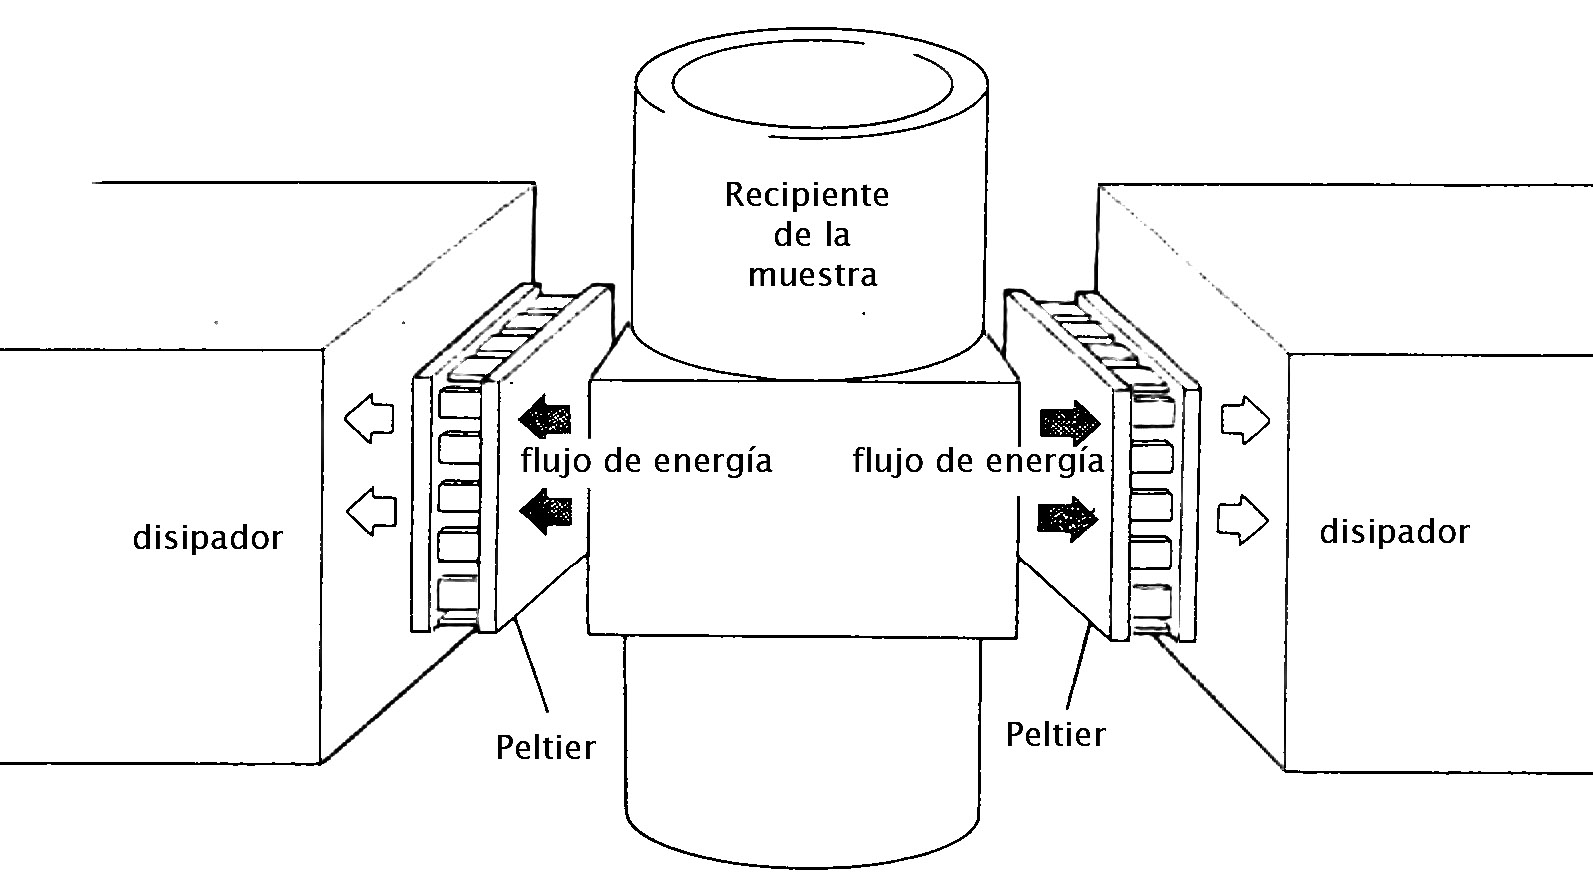
\includegraphics[width=\linewidth]{Figures/heatFlow}
			\caption{Interacci\'on de la celda de medici\'on con los alrededores, modificado de \cite{Suurkuusk}.}
			\label{fig: heatFlow}
		\end{subfigure}
		\begin{subfigure}{0.39\linewidth}
			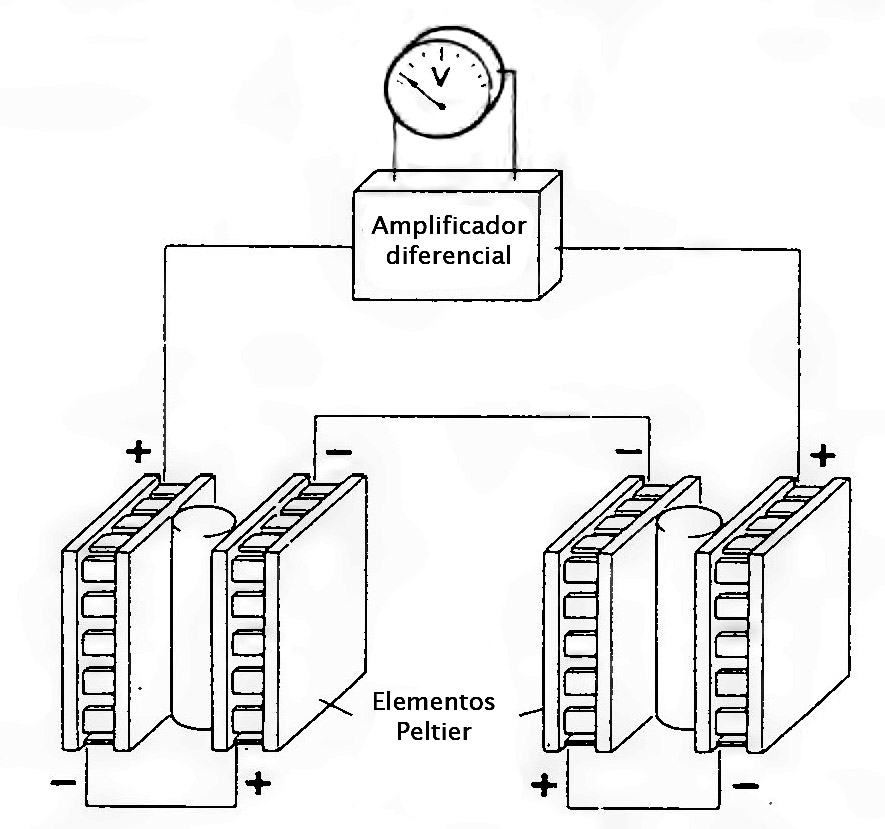
\includegraphics[width=\linewidth]{Figures/twinMeasuring}
			\caption{Principio de medici\'on de dos celdas gemelas, modificado de \cite{Suurkuusk}.}
			\label{fig: twin}
		\end{subfigure}
		\caption{Principio de detecci\'on de la energ\'ia transferida en forma de calor para cada canal de medida del calor\'imetro.}
	\end{figure}
	\newpage

	El calor\'imetro est\'a dise\~nado para que sea posible usar hasta cuatro cilindros de medici\'on independientes. Para cada uno de ellos, el principal camino del flujo de energ\'ia desde o hacia la celda es a trav\'es de los elementos Peltier \cite{Suurkuusk}. Dichos elementos est\'an compuestos de materiales semiconductores, sensibles a gradientes de temperatura del orden $1\times10^{-6}$ \grad{} \cite{Suurkuusk, simon2013oxford}. La uni\'on de estos semiconductores en serie, da lugar a detectores altamente sensibles a flujos de energ\'ia en forma de calor. Para detectar estos flujos se usa el efecto Seebeck, seg\'un el cual, para un gradiente de temperatura se genera una diferencia de potencial entre dos terminales de la celda. El efecto contrario recibe el nombre de efecto Peltier y se debe a que al pasar una corriente el\'ectrica a trav\'es de un material, se genera un transporte de energ\'ia en forma de calor. El flujo de energ\'ia t\'ermica se escribe de la siguiente forma \cite{simon2013oxford}:
	\begin{equation}\label{eq: peltier}
		\mathbf{j}^q = \Pi \mathbf{j}
	\end{equation}
	
	donde $\Pi$ recibe el nombre de coeficiente Peltier, $\mathbf{j}^q$ es la densidad de flujo de energ\'ia en forma de calor y $\mathbf{j}$ la densidad de corriente el\'ectrica \cite{simon2013oxford}. El coeficiente Seebeck ($S$) se define como $S = -\Delta V/\Delta T$ con $\Delta V$ como la diferencia de voltaje y se relaciona con el coeficiente de Peltier como: $\Pi = ST$, por lo cual al aplicar sobre la \autoref{eq: peltier} se obtiene:
	\begin{equation}\label{eq: seebeck}
		\mathbf{j}^q = (ST) \mathbf{j} = \left(-T\dfrac{\mathbf{j}}{\Delta T}\right)\Delta V = k\Delta V
	\end{equation}
	
	De esta forma se tiene que $\mathbf{j}^q \propto \Delta V$, por lo cual es posible cuantificar un flujo de energ\'ia t\'ermica en forma de calor con una lectura de potencial el\'ectrico. Las calibraciones el\'ectricas permiten determinar el valor de $k$, el cual, como se observa en la \autoref{eq: seebeck}, depende de la temperatura, por lo cual si se modifica la temperatura del ba\~no interno resulta necesario realizar una nueva calibraci\'on el\'ectrica. Dada esta dependencia con la temperatura, el calor\'imetro cuenta con un ba\~no termostatado con capacidad para 25 litros de agua, los cuales rodean los cilindros de medici\'on y act\'ua como reservorio t\'ermico \cite{Suurkuusk}. La sensibilidad a la temperatura hace que las funciones principales del calor\'imetro se encuentren divididas en dos unidades independientes, la del control de las condiciones isot\'ermicas y la detecci\'on de los eventos calorim\'etricos. La primera se encuentra descrita en el \autoref{ch: thermal}. Respecto a la segunda, la detecci\'on de los flujos de energ\'ia en forma de calor, el calor\'imetro usa dos celdas de medici\'on para cada canal de medida. Los elementos Peltier de cada canal se encuentran conectados en serie, pero con la polarizaci\'on opuesta, de tal forma que se registre la diferencia en los flujos de calor de las dos celdas, de esta forma es posible usar una para el estudio de la muestra (lado \texttt{A}) y otra para realizar un blanco (lado \texttt{B}) como se muestra en la \autoref{fig: twin}.
	 
	El calor\'imetro puede tomar medidas de ampollas, las cuales pueden ser usadas para estudiar el crecimiento de microorganismos, o en modo de titulaci\'on, para el cual es necesario contar con un agitador permanente en la soluci\'on, as\'i como de un sistema de inyecci\'on para adicionar la soluci\'on titulante \cite{Suurkuusk}. Un ejemplo de esta aplicaci\'on es la calibraci\'on qu\'imica que se muestra en el \autoref{ch: chemical}, de donde se pueden obtener propiedades termodin\'amicas del sistema a partir de la potencia registrada este. 	 

\section{Justificación del proyecto}
	En general, la calorimetría permite una gran variedad de análisis, muchos de ellos cuentan con aplicaciones industriales, comerciales, biológicos y químicos, permitiendo el entendimiento de las interacciones moleculares en soluciones \cite{blandamer1998titration}. Una ventaja de la calorimetría es que no es específica, ni invasiva, además de no depender de las propiedades electroquímicas y ópticas de un sistema dado, siendo esto de vital importancia para las investigaciones de procesos biológicos, el estudio del crecimiento bacteriano y para la detección de compuestos biológicos \cite{winkelmann2004application}. Por otro lado la calorimetría también permite el estudio de la termodinámica en sistemas de absorción, bien sea por la universalidad de la absorción física en superficies como catalizadores, o en procesos industriales como la separación de mezclas de gases \cite{morrison1987calorimetry}. Finalmente la calorimetría es el método clásico para la determinación de propiedades termodinámicas en las muestras, entre estas se encuentran: capacidad calorífica, entalpía, entropía y energía libre de Gibbs, las cuales constituyen el punto de partida de gran cantidad de estudios teóricos, desarrollos y producción industrial de un compuesto químico \cite{wang2005determination, gaisford2016principles}.
	
	El calorímetro 2277 Thermal Activity Monitor con el que cuenta el grupo de investigación, al momento de realizar este trabajo se encontraba desarmado, a la espera de su instalaci\'on y puesta en funcionamiento. Este instrumento permite monitorear una gran variedad de reacciones químicas y bioquímicas, lo anterior debido a su capacidad de cuantificar procesos exotérmicos y endotérmicos. Estas reacciones pueden ser estudiadas en el rango de 5 - 80 $^\circ$C \cite{Suurkuusk}. Este rango de temperaturas se debe al uso de un baño termostatado de 25 litros. Cuatro balones de medición independientes se encuentran sumergidos en este baño, permitiendo medidas en el rango de microvatios \cite{Suurkuusk}. Es por esta razón que poner en marcha y calibrar el equipo con el que cuenta el grupo de investigación resulta una contribución importante para el mismo, así como para el \deptname\ en general.
	
\section{Objetivos}
	\subsection{Objetivo general}
		Poner en funcionamiento el calorímetro 2277 Thermal Activity Monitor con el que se cuenta, y adicionalmente calibrar el equipo para su uso en las investigaciones activas del grupo \groupname.
		
	\subsection{Objetivos específicos}
		\begin{itemize}
			\item Realizar el cableado y conexiones electrónicas pertinentes a la instalaci\'on del equipo 2277 Thermal Activity Monitor.
			\item Mantener la temperatura del ba\~no interno estable a una temperatura de 25 \grad{}.
			\item Realizar calibraciones eléctricas, para asegurar que las señales obtenidas tengan un equivalente en potencia.
			\item Determinación de la entalpía molar, energía libre de Gibbs, entropía, y constante de afinidad, de la reacci\'on de bicarbonato de potasio con \'acido clorh\'idrico como una calibración química.
		\end{itemize}
	
	
%\section{Metodología}
%	Para el ensamble del calorímetro se cuenta con el catálogo de partes, y el manual de instrucciones. En el primero se detallan y enumeran las partes del equipo, en la \autoref{fig:partes} se muestran ejemplos de los distintos sistemas con los que el calorímetro cuenta \cite{Suurkuusk}. 
%	
%	\begin{figure}[h]
%		\centering
%		\begin{subfigure}[b]{0.3\textwidth}
%			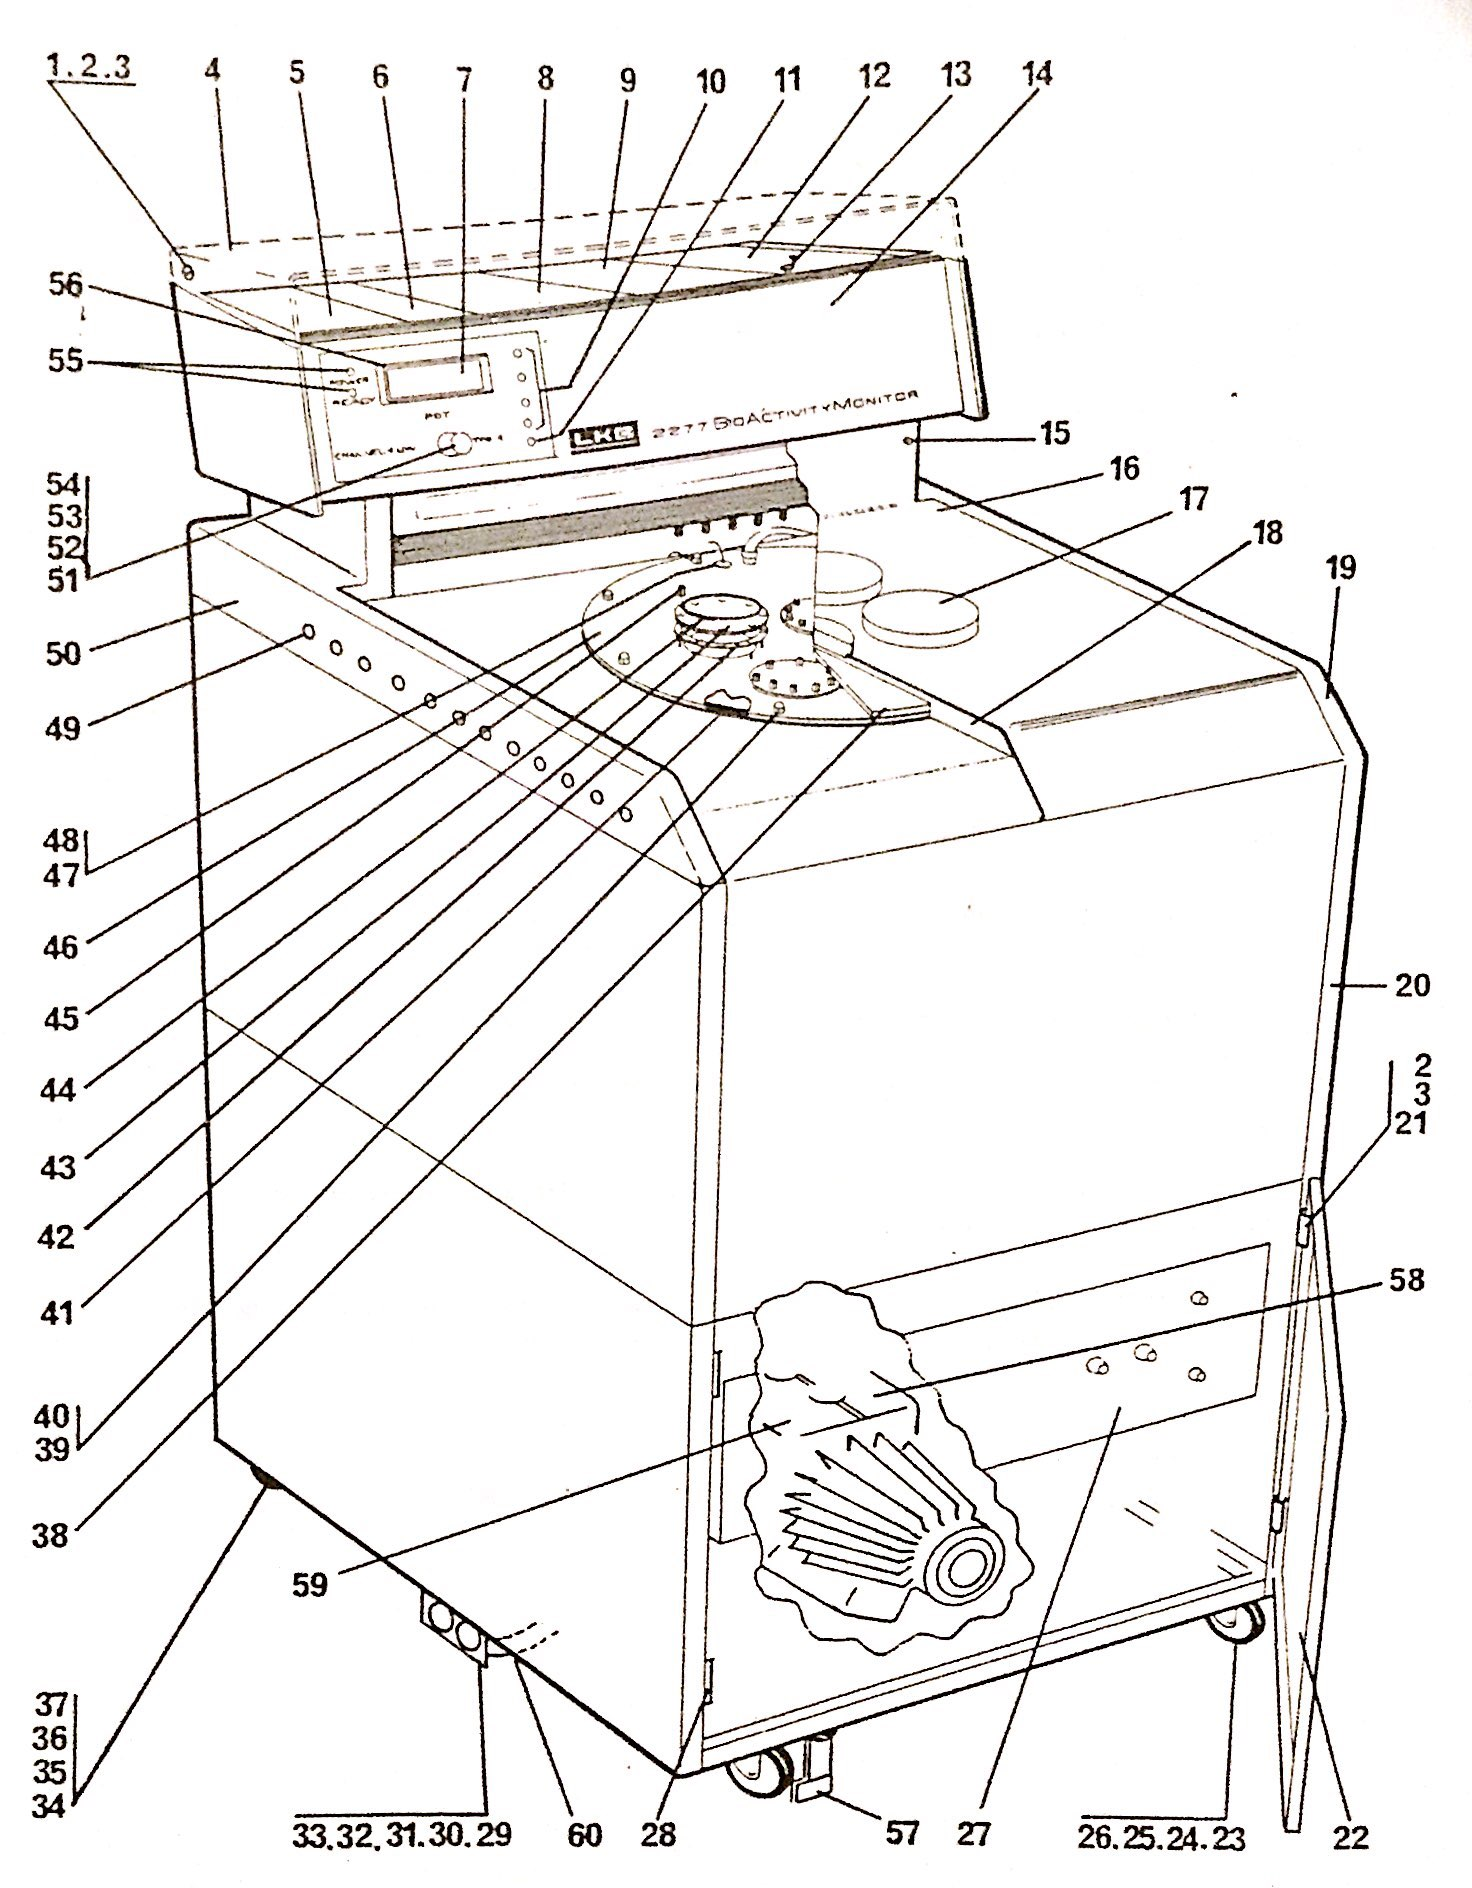
\includegraphics[width=\textwidth]{Figures/images_1.jpg}
%			\caption{Vista exterior del equipo con sus componentes.}
%			\label{fig:vistaExterior}
%		\end{subfigure}
%		~ 
%		\begin{subfigure}[b]{0.37\textwidth}
%			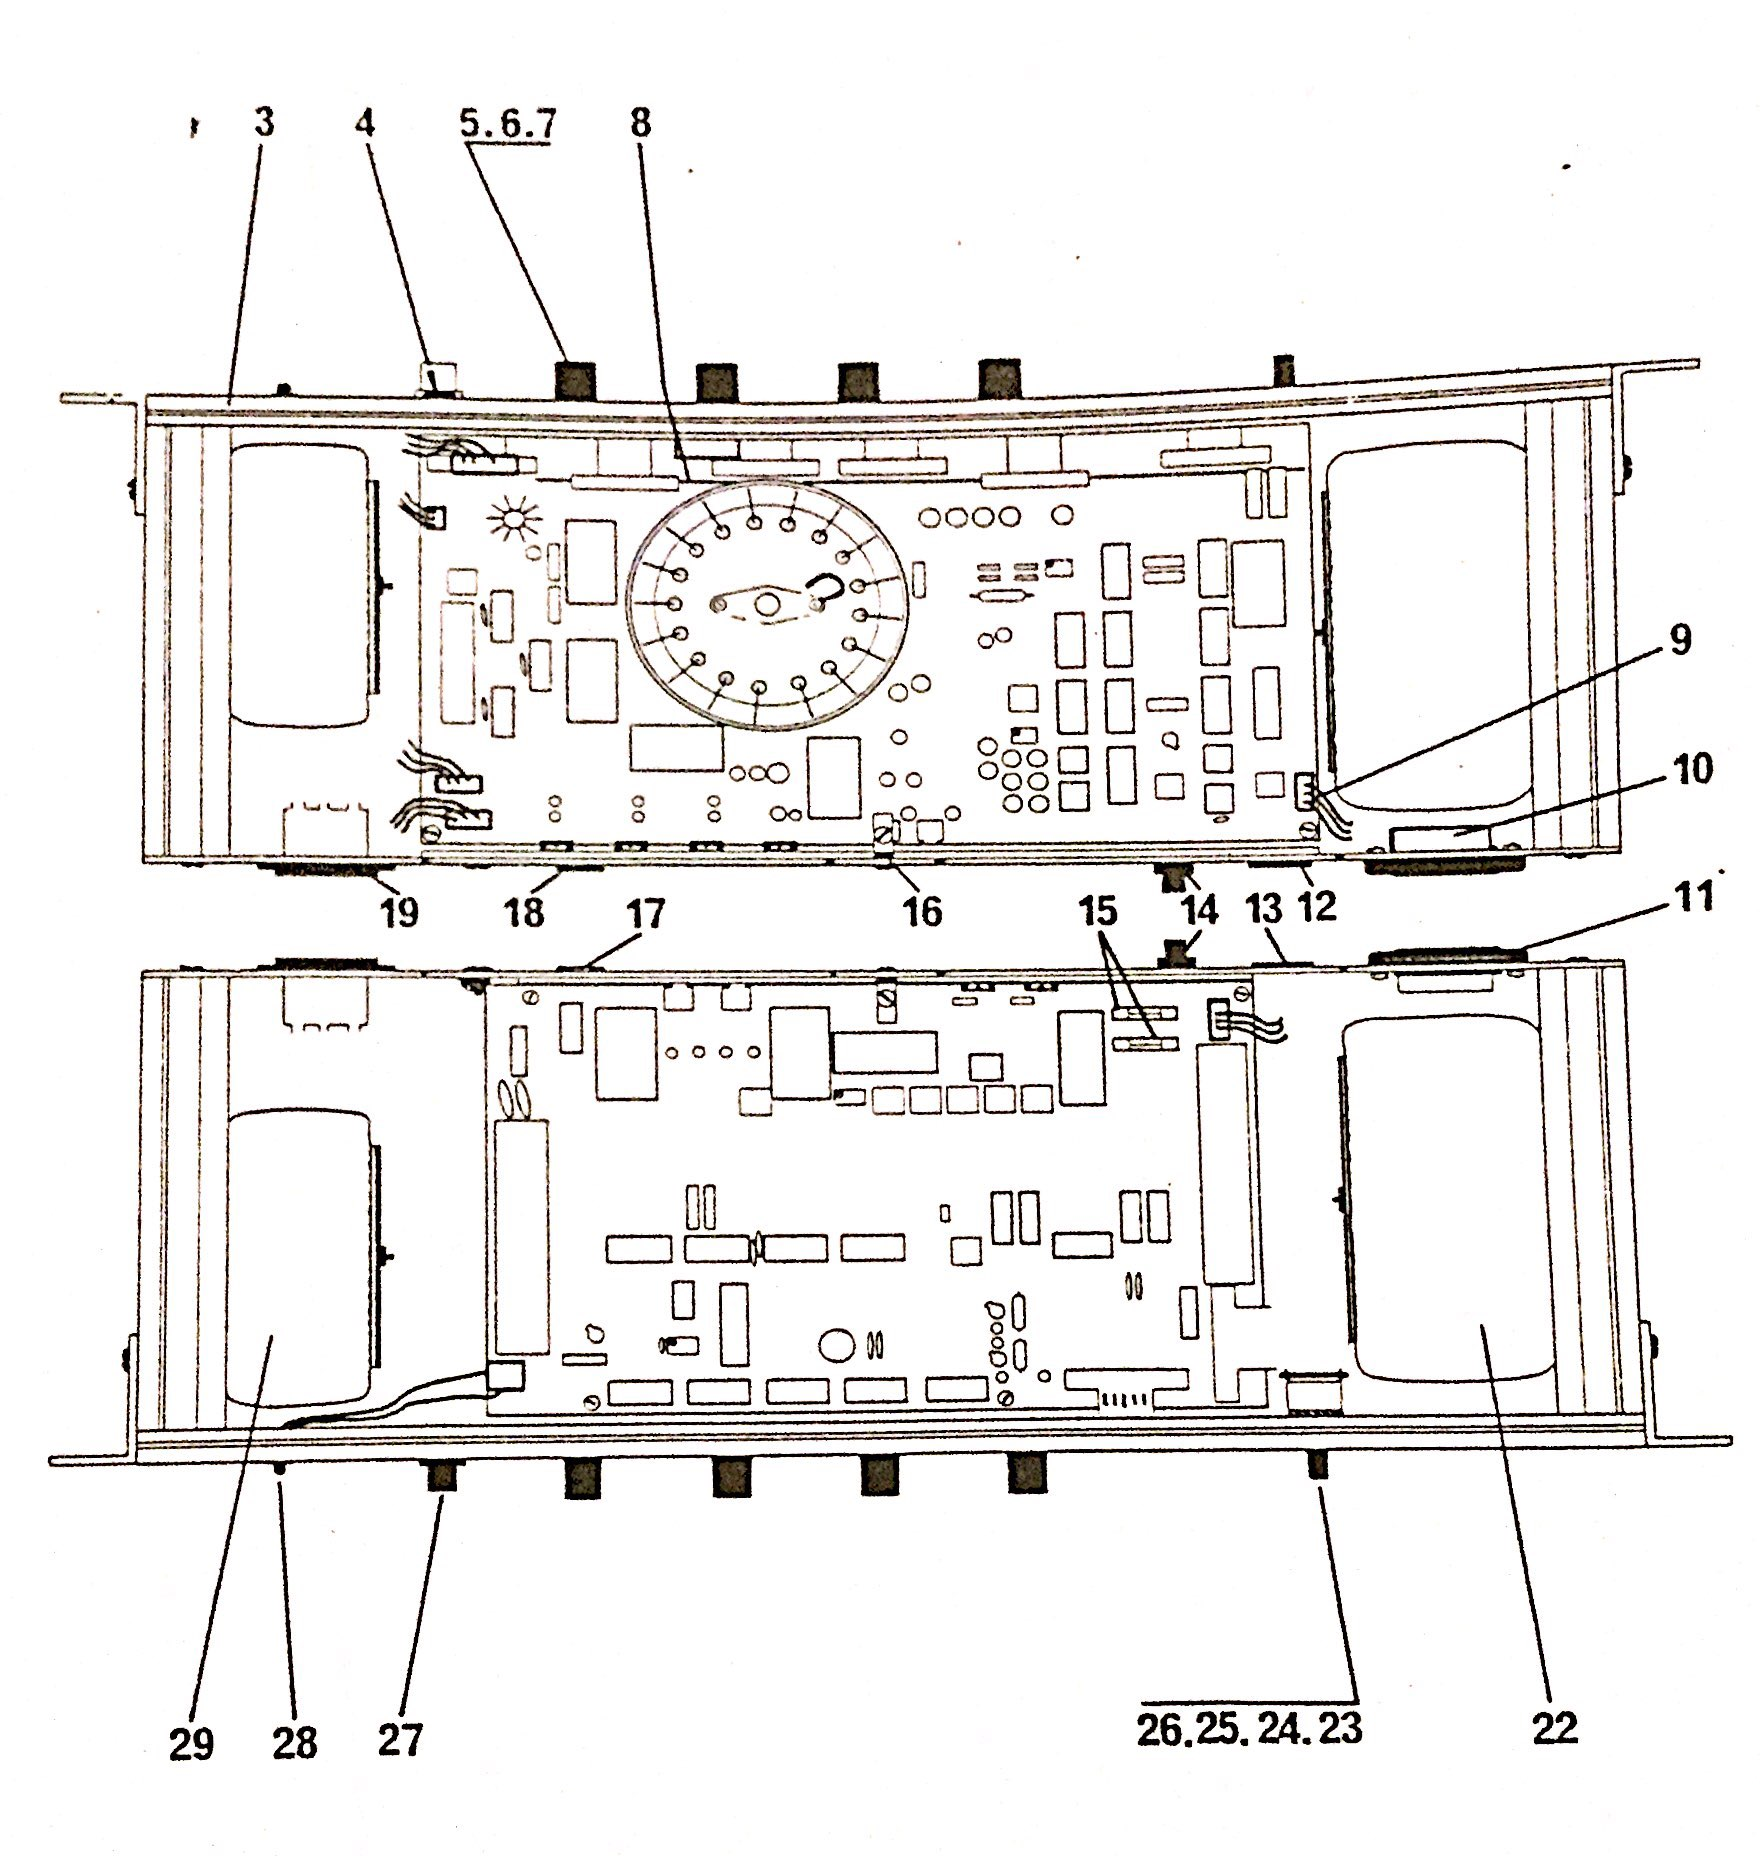
\includegraphics[width=\textwidth]{Figures/images_2.jpg}
%			\caption{Parte del sistema eléctrico del calorímetro.}
%			\label{fig:sistemaElectrico}
%		\end{subfigure}
%		~ 
%		\begin{subfigure}[b]{0.25\textwidth}
%			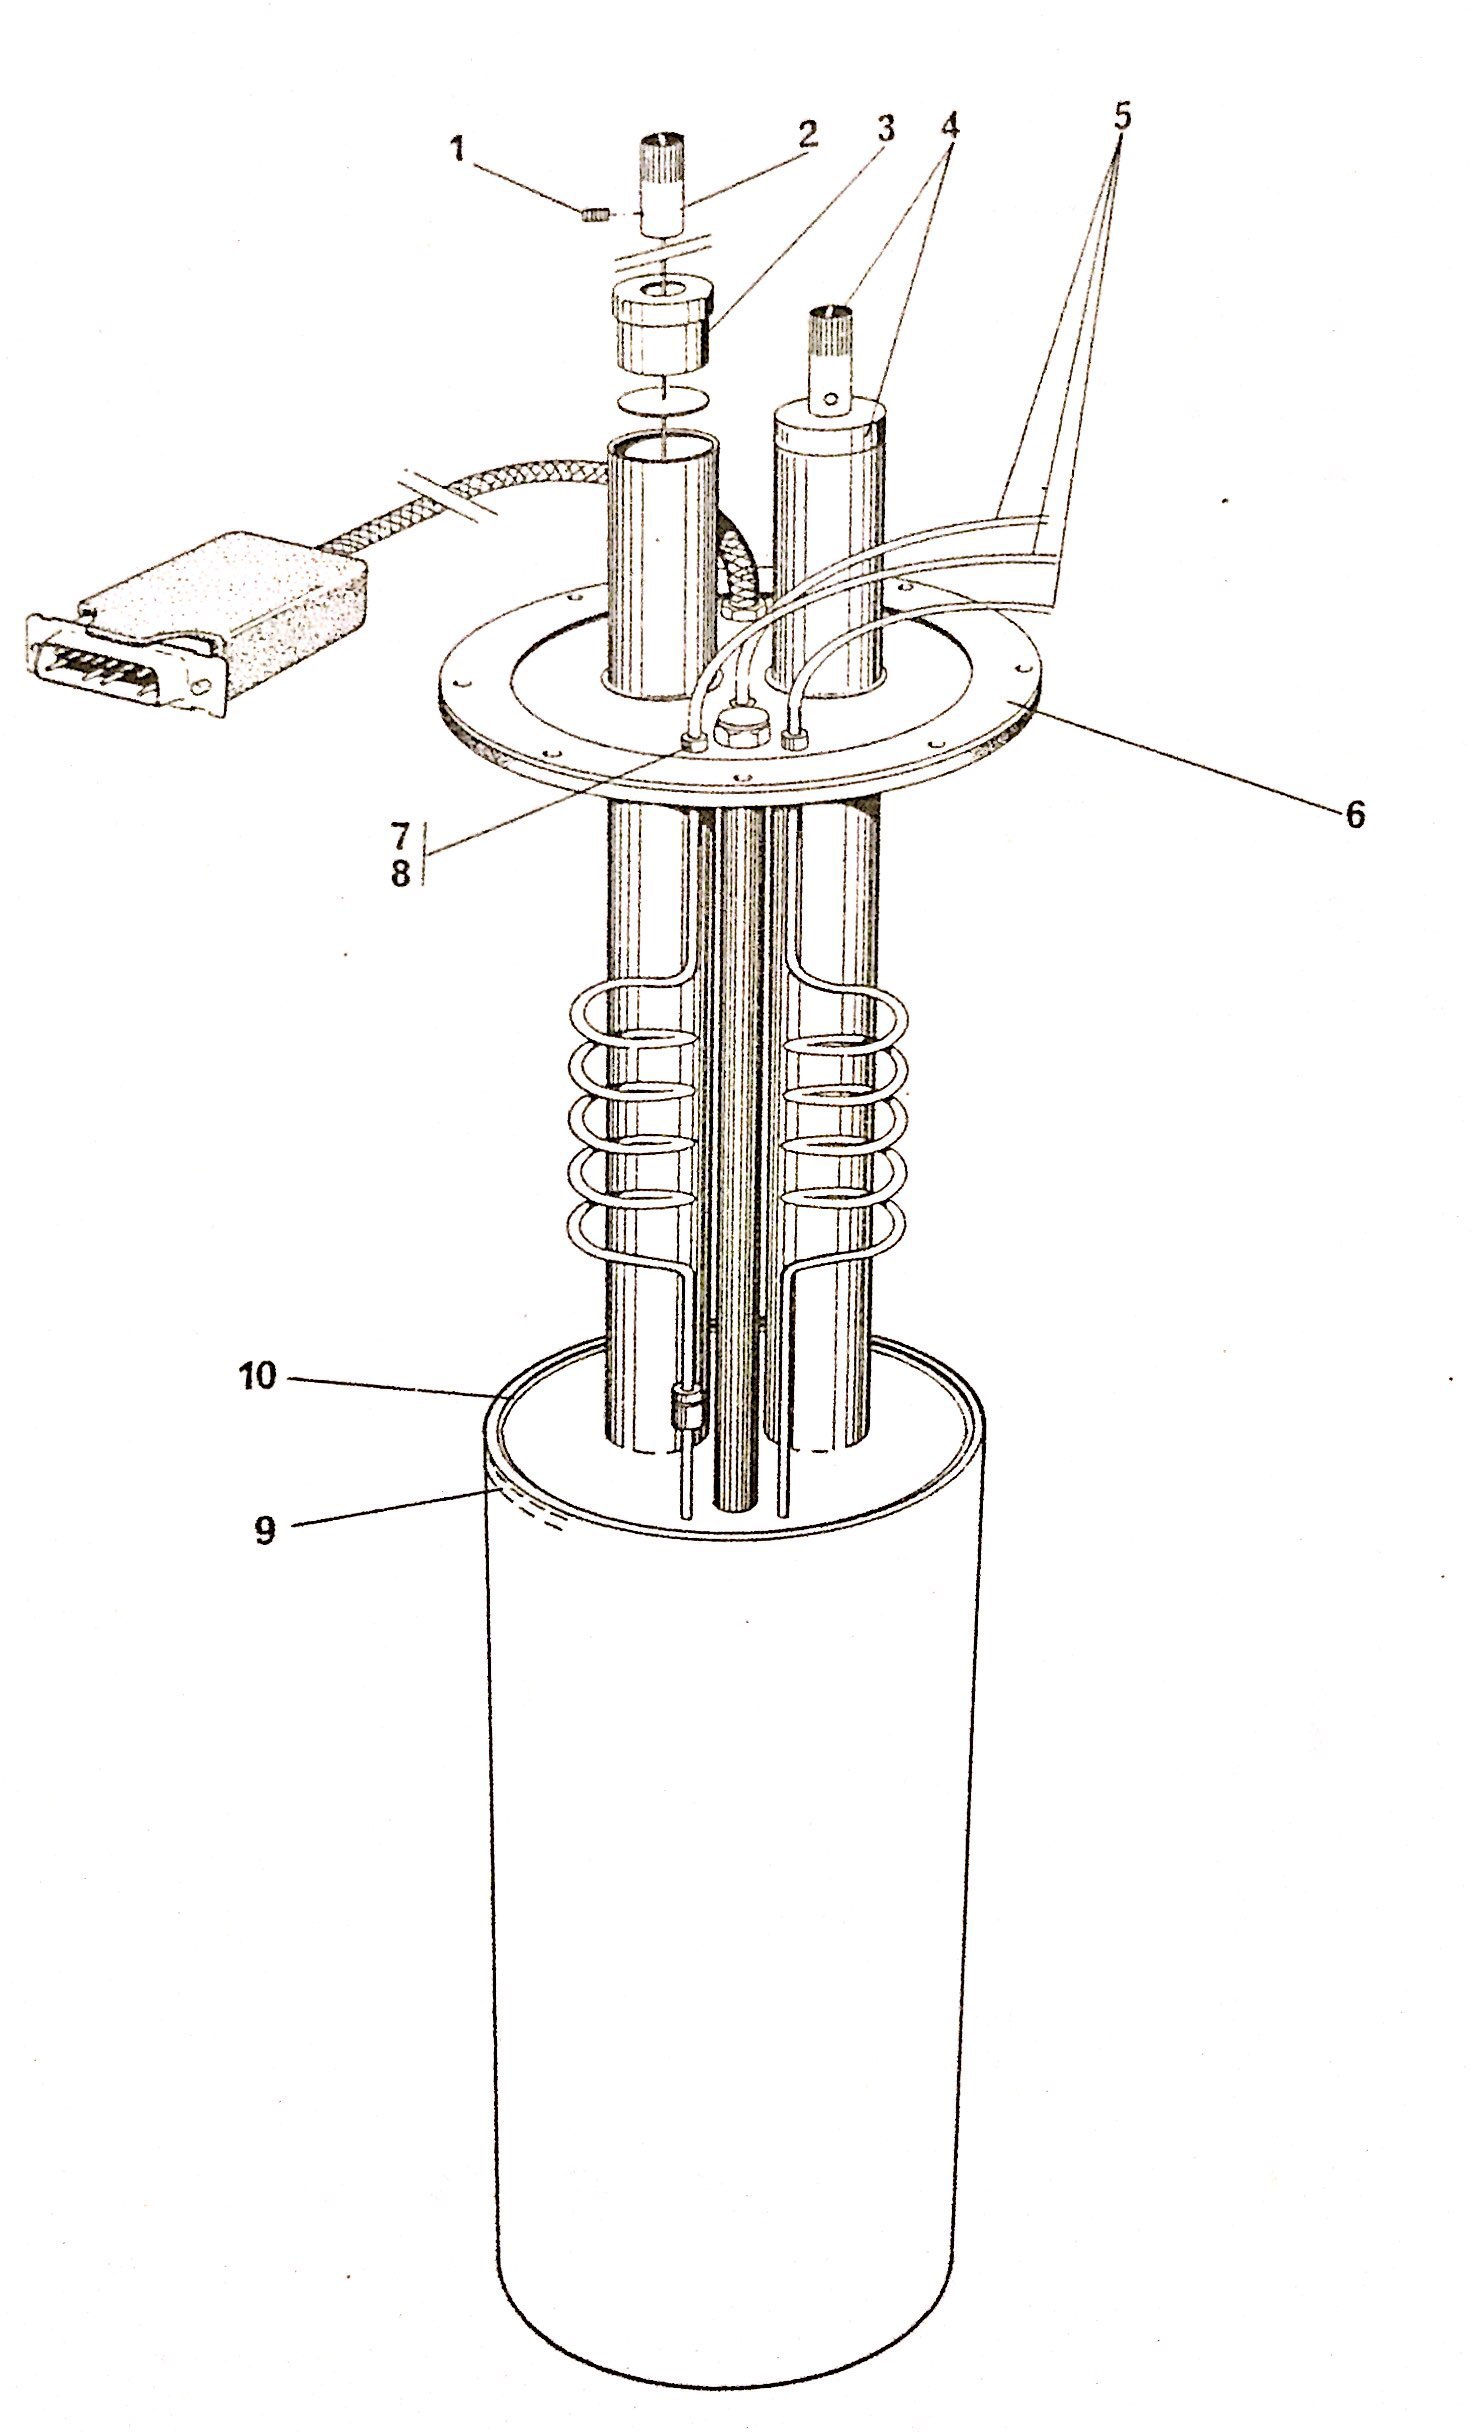
\includegraphics[width=\textwidth]{Figures/images_3.jpg}
%			\caption{Celda de medición.}
%			\label{fig:celda}
%		\end{subfigure}
%		\caption{Componentes exteriores del equipo y partes de los sistemas del calorímetro \cite{Suurkuusk}.}
%		\label{fig:partes}
%	\end{figure}
%	Usando esta información se llevará a cabo el ensamble del calorímetro así como las conexiones eléctricas.	A nivel electrónico, la liberación o absorción de energía térmica se mide usando una celda Peltier, las cuales tienen una respuesta proporcional en voltaje, de esta forma se obtiene una señal eléctrica a partir de pequeñas variaciones de temperatura en la celda de reacción. La señal eléctrica es procesada por el sistema digital del instrumento \cite{Suurkuusk}. De esta forma y siguiendo las instrucciones es posible realizar una calibración eléctrica del sistema.
%	
%	La calibración química puede realizarse de distintas maneras. En principio cualquier reacción que pueda ser llevada a cabo en un calorímetro, con condiciones controladas y cuyas propiedades termodinámicas sean bien conocidas, puede ser usada como una reacción de calibración \cite{wadso2001standards}. Sin embargo es recomendable que los reactivos involucrados en estas reacciones no requieran de algún tipo de purificación que pueda alterar el análisis \cite{wadso2001standards}.
%	
%	Se propone realizar una calorimetría de titulación como método de calibración química, lo anterior es importante porque una calibración eléctrica puede dar lugar a distribuciones de temperatura distintas en la celda de reacción, o generar patrones de flujo de calor distintos a una reacción química, esto puede generar errores sistemáticos en las medidas realizadas \cite{wadso2001standards}. La titulación es una técnica importante en la medida que permite la determinación simultánea de la entalpía molar y la constante de equilibrio de la reacción, por lo cual también se obtienen el cambio en la energía estándar de Gibbs y el cambio en la entropía estándar \cite{wadso2001standards}. 
%	
%	Para esta calibración es necesario contar con soluciones acuosas de cloruro de bario (\ce{BaCl2}) y éter 18-corona-6 (\ce{[C2H4O]6}) \cite{tellinghuisen2007optimizing, mizoue2004calorimetric, wadso2001standards}. La reacción de acomplejamiento es 1:1, de la siguiente forma:
%	\begin{equation}
%		\ce{Ba^{2+}(ac) + [C2H4O]6(ac) -> Ba^{2+}.[C2H4O]6(ac)}
%	\end{equation}
%	
%	Dichas soluciones deben encontrarse en el rango de concentraciones de 1 mM a 10 mM para el éter y 10 mM hasta 100 mM para el cloruro de bario. Dentro de este rango, existe evidencia experimental que muestra que no hay una variación significativa de las cantidades termodinámicas medidas \cite{wadso2001standards, mizoue2004calorimetric}. Considerando el volumen de las celdas con las que cuenta el equipo, se propone usar 1.5 mL de la solución de éter. Las soluciones deben ser desgasificadas y  termostatadas a 25 $^\circ$C, con el objetivo de limitar el error experimental introducido por diferencias de temperatura causadas por burbujas \cite{mizoue2004calorimetric, tellinghuisen2007optimizing, duff2011isothermal}. 
%	
%	En el calorímetro el ba\~no debe encontrarse a 25 $^\circ$C y deben usarse dos de las cuatro celdas disponibles. La primera se considera como referencia y debe contener al disolvente únicamente, en este caso 1.5 mL de agua \cite{Suurkuusk}. En la segunda se adiciona el mismo volumen de la solución de éter, una vez la línea base del calorímetro se encuentra estable, se adicionan una a una 30 alícuotas de la solución de cloruro de bario, con tiempos entre inyección mayores a $\tau = 6$ minutos, tanto a la celda de referencia como a la de reacción \cite{mizoue2004calorimetric, duff2011isothermal}. Cada inyección modifica la temperatura de la celda respecto a la referencia, razón por la cual las termopilas Peltier, deberán compensarla, la energía requerida por las celdas se cuantifica en función del tiempo, esto da lugar a una gráfica de potencia en función del tiempo \cite{duff2011isothermal}. Para cada inyección, es posible calcular el cambio en la energía integrando la potencia usada por el sistema. La gráfica de los cambios energéticos en función de la fracción molar (\ce{[Ba^{2+}]}/[éter]) permite obtener  las propiedades termodinámicas \cite{duff2011isothermal, mizoue2004calorimetric}. La diferencia entre el valor mínimo de la isotérma y la línea base de esta corresponde con la entalpía molar estándar $\Delta H_m$. La derivada de la isotérma en el punto equimolar, da lugar a la constante de afinidad $K_a$. Finalmente con esta es posible determinar los cambios en la energía libre de Gibbs y la entropía.
%	
%	\begin{equation}
%		\Delta G_m = -RT\ln K_a = \Delta H_m - T\Delta S_m
%	\end{equation}
%	
%	Para determinar la capacidad calorífica es necesario realizar el mismo experimento a distintas temperaturas, dado que:
%	\begin{equation}
%		C_{p, m} = \left(\dfrac{\partial H_m}{\partial T}\right)_p
%	\end{equation}
%	
%	En el caso de esta titulación los valores reportados por IUPAC corresponden con \cite{wadso2001standards}:
%	\begin{itemize}
%		\item $\Delta H_m = -(31.42 \pm 0.20)$ kJ mol$^{-1}$
%		\item $K_a = (5.90 \pm 0.20)\times10^3$ mM
%		\item $C_{p,m} = 126$ J K$^{-1}$ mol$^{-1}$
%	\end{itemize}
% !TeX spellcheck = es_ES
% Chapter 1

%\chapter{Chapter Title Here} % Main chapter title
%
%\label{Chapter1} % For referencing the chapter elsewhere, use \ref{Chapter1} 

%----------------------------------------------------------------------------------------

% Define some commands to keep the formatting separated from the content 
%\newcommand{\keyword}[1]{\textit{#1}}
%\newcommand{\tabhead}[1]{\textbf{#1}}
%\newcommand{\code}[1]{\texttt{#1}}
%\newcommand{\file}[1]{\texttt{\bfseries#1}}
%\newcommand{\option}[1]{\texttt{\itshape#1}}

%----------------------------------------------------------------------------------------

\chapter{Instalación del calorímetro}
	El calorímetro originalmente era usado en la Universidad Sueca de Ciencias Agrícolas, en donde la red eléctrica es de 230 VAC. En Colombia se usan 110 VAC, razón por la cual una parte importante de la instalación del calorímetro consistió en configurar las entradas de voltaje del equipo para su operación en el país. Para esto fue necesario cambiar 2 fusibles por unos con capacidad para el doble de corriente, pues en los circuitos eléctricos con transformadores que permiten ajustar el voltaje de entrada, se tiene que conservar la potencia, la cual está dada por el producto de corriente y voltaje. Los fusibles se encuentran en el panel inferior derecho del calorímetro (\autoref{fig: fuseBox}), y en la parte trasera, los nuevos fusibles tienen valores de corriente de 4 A y 6 A, correspondientemente. Junto con este cambio fue necesario modificar las perillas selectoras de voltaje, una de las cuales se encuentra en el mismo panel del primer fusible (\autoref{fig: fuseBox}) mientras que el otro está en la parte trasera del módulo de control de la temperatura (\autoref{fig: decadeResistors}), el valor seleccionado es de 115 VAC.
	\begin{figure}[h]
		\centering
		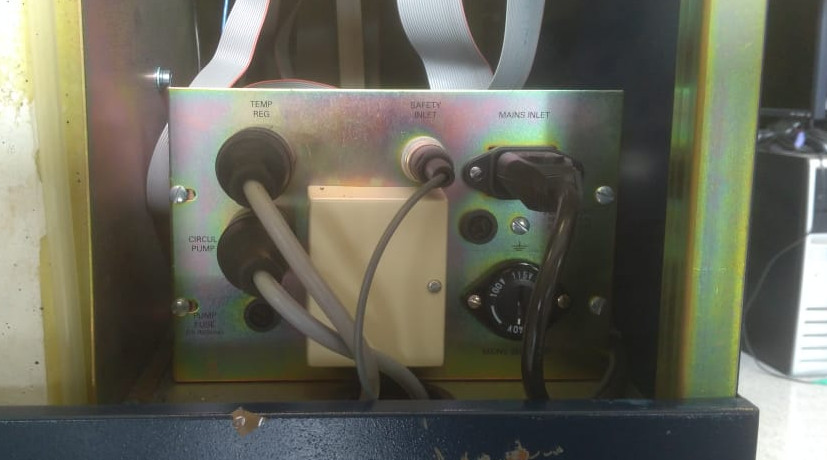
\includegraphics[width=0.7\linewidth]{Figures/fusepanel}
		\caption{Panel de selección de voltaje del calorímetro.}
		\label{fig: fuseBox}
	\end{figure}

	Posteriormente, uno de los cilindros de medición fue identificado en una de las cajas, se fijó al baño interno, y se llevaron a cabo las conexiones eléctricas con el módulo de amplificación como se muestra a continuación. 
	\begin{figure}[h]
		\centering
		\begin{tabular}{cccc}
			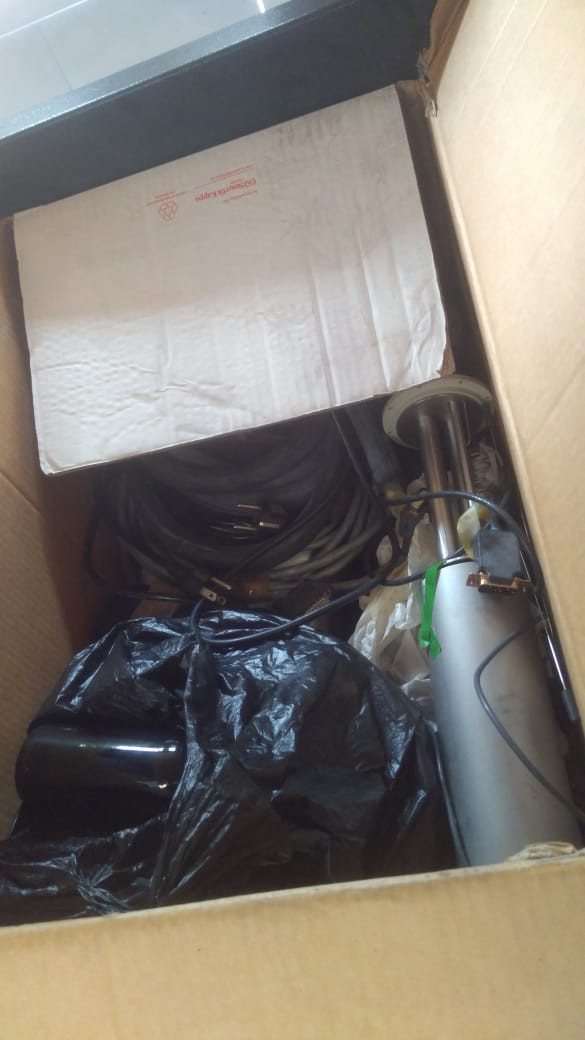
\includegraphics[width=0.24\linewidth]{Figures/process/box1} & 
			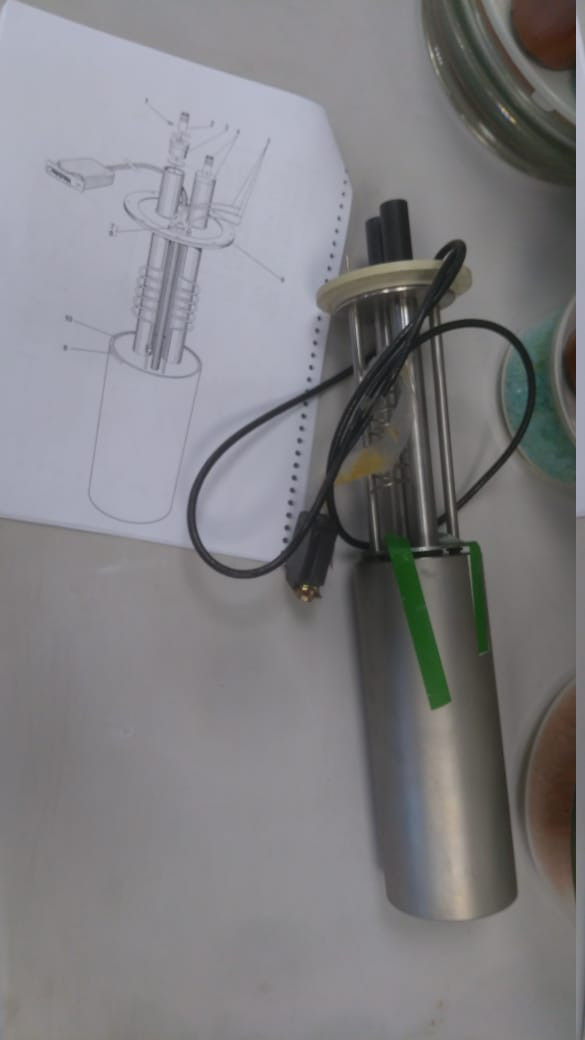
\includegraphics[width=0.24\linewidth]{Figures/process/holder} &
			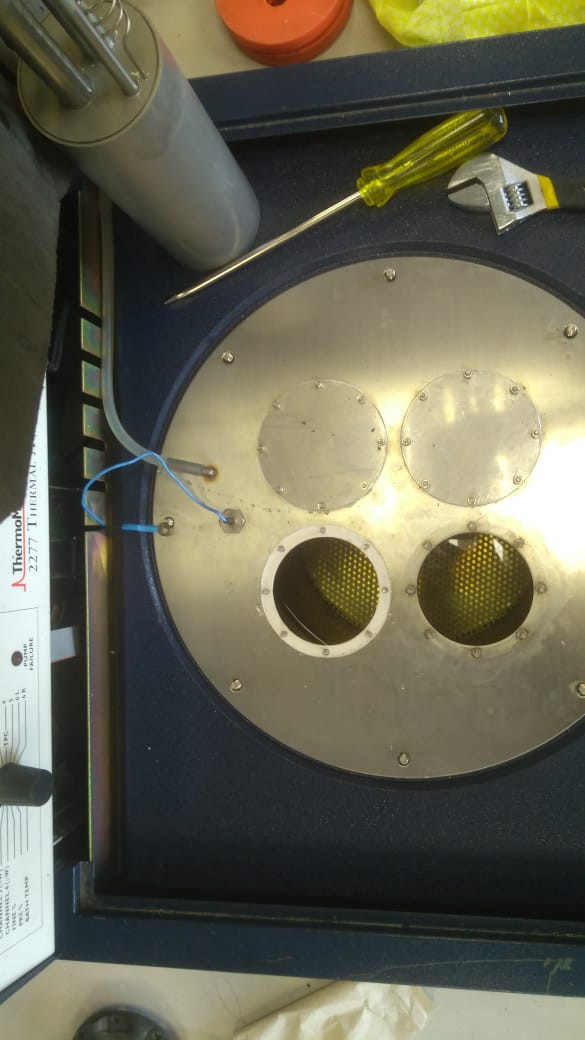
\includegraphics[width=0.24\linewidth]{Figures/process/p1} & 
			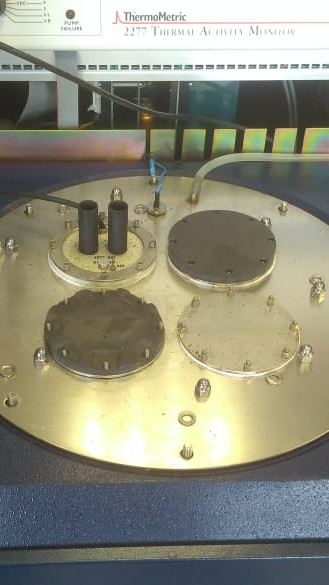
\includegraphics[width=0.24\linewidth]{Figures/process/p2} \\
			& 
			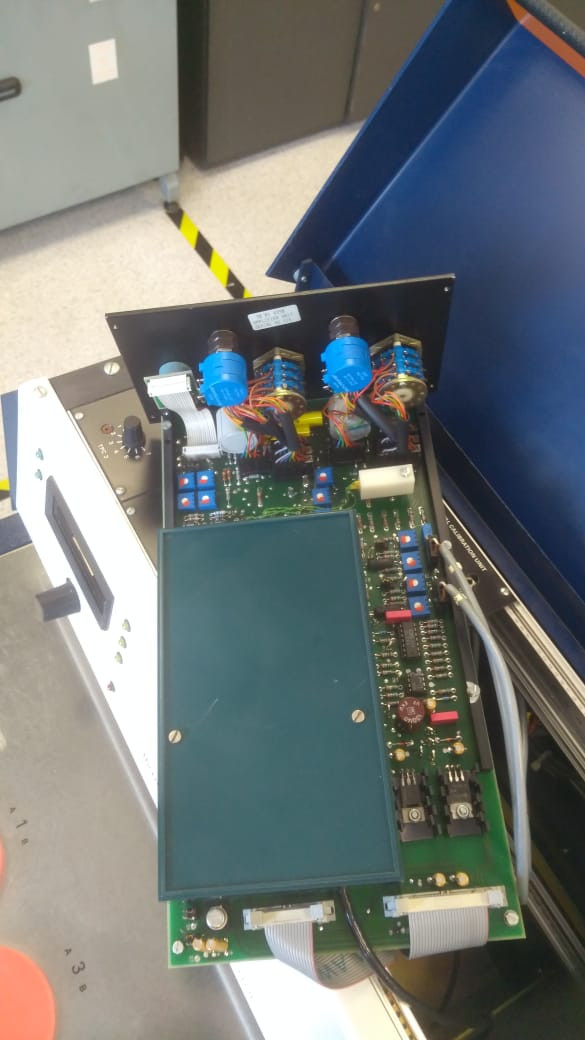
\includegraphics[width=0.24\linewidth]{Figures/process/p3} &
			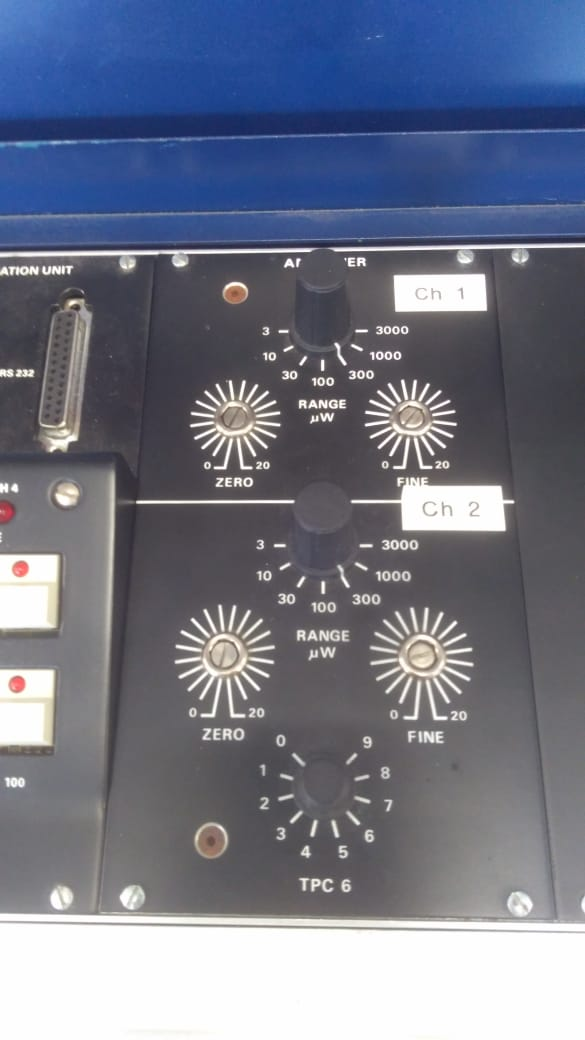
\includegraphics[width=0.24\linewidth]{Figures/process/p4} &
		\end{tabular}
		\caption{Proceso de instalación de un cilindro de medición.}
		\label{fig: instalationMultiple}
	\end{figure}

	Una vez instalado el cilindro se adicionaron cerca de 25 litros de agua al calor\'imetro usando uno de los orificios que se observa en la \autoref{fig: connection}, y se conectaron las mangueras del baño externo al equipo, cuya conexión se encuentra en la parte inferior del lado izquierdo del calorímetro. Donde el flujo de entrada corresponde con la manguera derecha. Posteriormente el sistema fue encendido y se verific\'o que este registrara la temperatura del ba\~no interno, el valor de la temperatura fue corroborado usando un term\'ometro de mercurio con longitud de 76 mm y nitr\'ogeno gaseoso en su interior, cuyas temperaturas de trabajo se encuentran entre -1,0 \grad{} a 51,0 \grad{} y precisión de 0,1 \grad{} )referencia \texttt{SAMA-CP40-N16B}), encontr\'andose que el calor\'imetro registra una temperatura 0,1 \grad{} superior a aquella medida por el term\'ometro de mercurio.
	
	La conexión con el computador se realiza usando el puerto RS232, que trae el calorímetro, y un conversor de protocolo RS232 a USB. De manera similar se realiza la comunicación con el controlador de la bomba de la jeringa, siendo este el único equipo que no fue posible adaptar a la red eléctrica colombiana, pues su voltaje de operaci\'on es \'unico, por lo cual, su uso requiere de un transformador eléctrico de 110 VAC a 230 VAC. Para el agitador originalmente era necesario el uso de un adaptador de 230 VAC a 5 VDC, pero dado que el voltaje que provee un puerto USB corresponde a este valor, se cambiaron las conexiones de tal forma que ahora solo es necesario conectar el agitador a un puerto de este tipo.
	\begin{figure}[h]
		\centering
		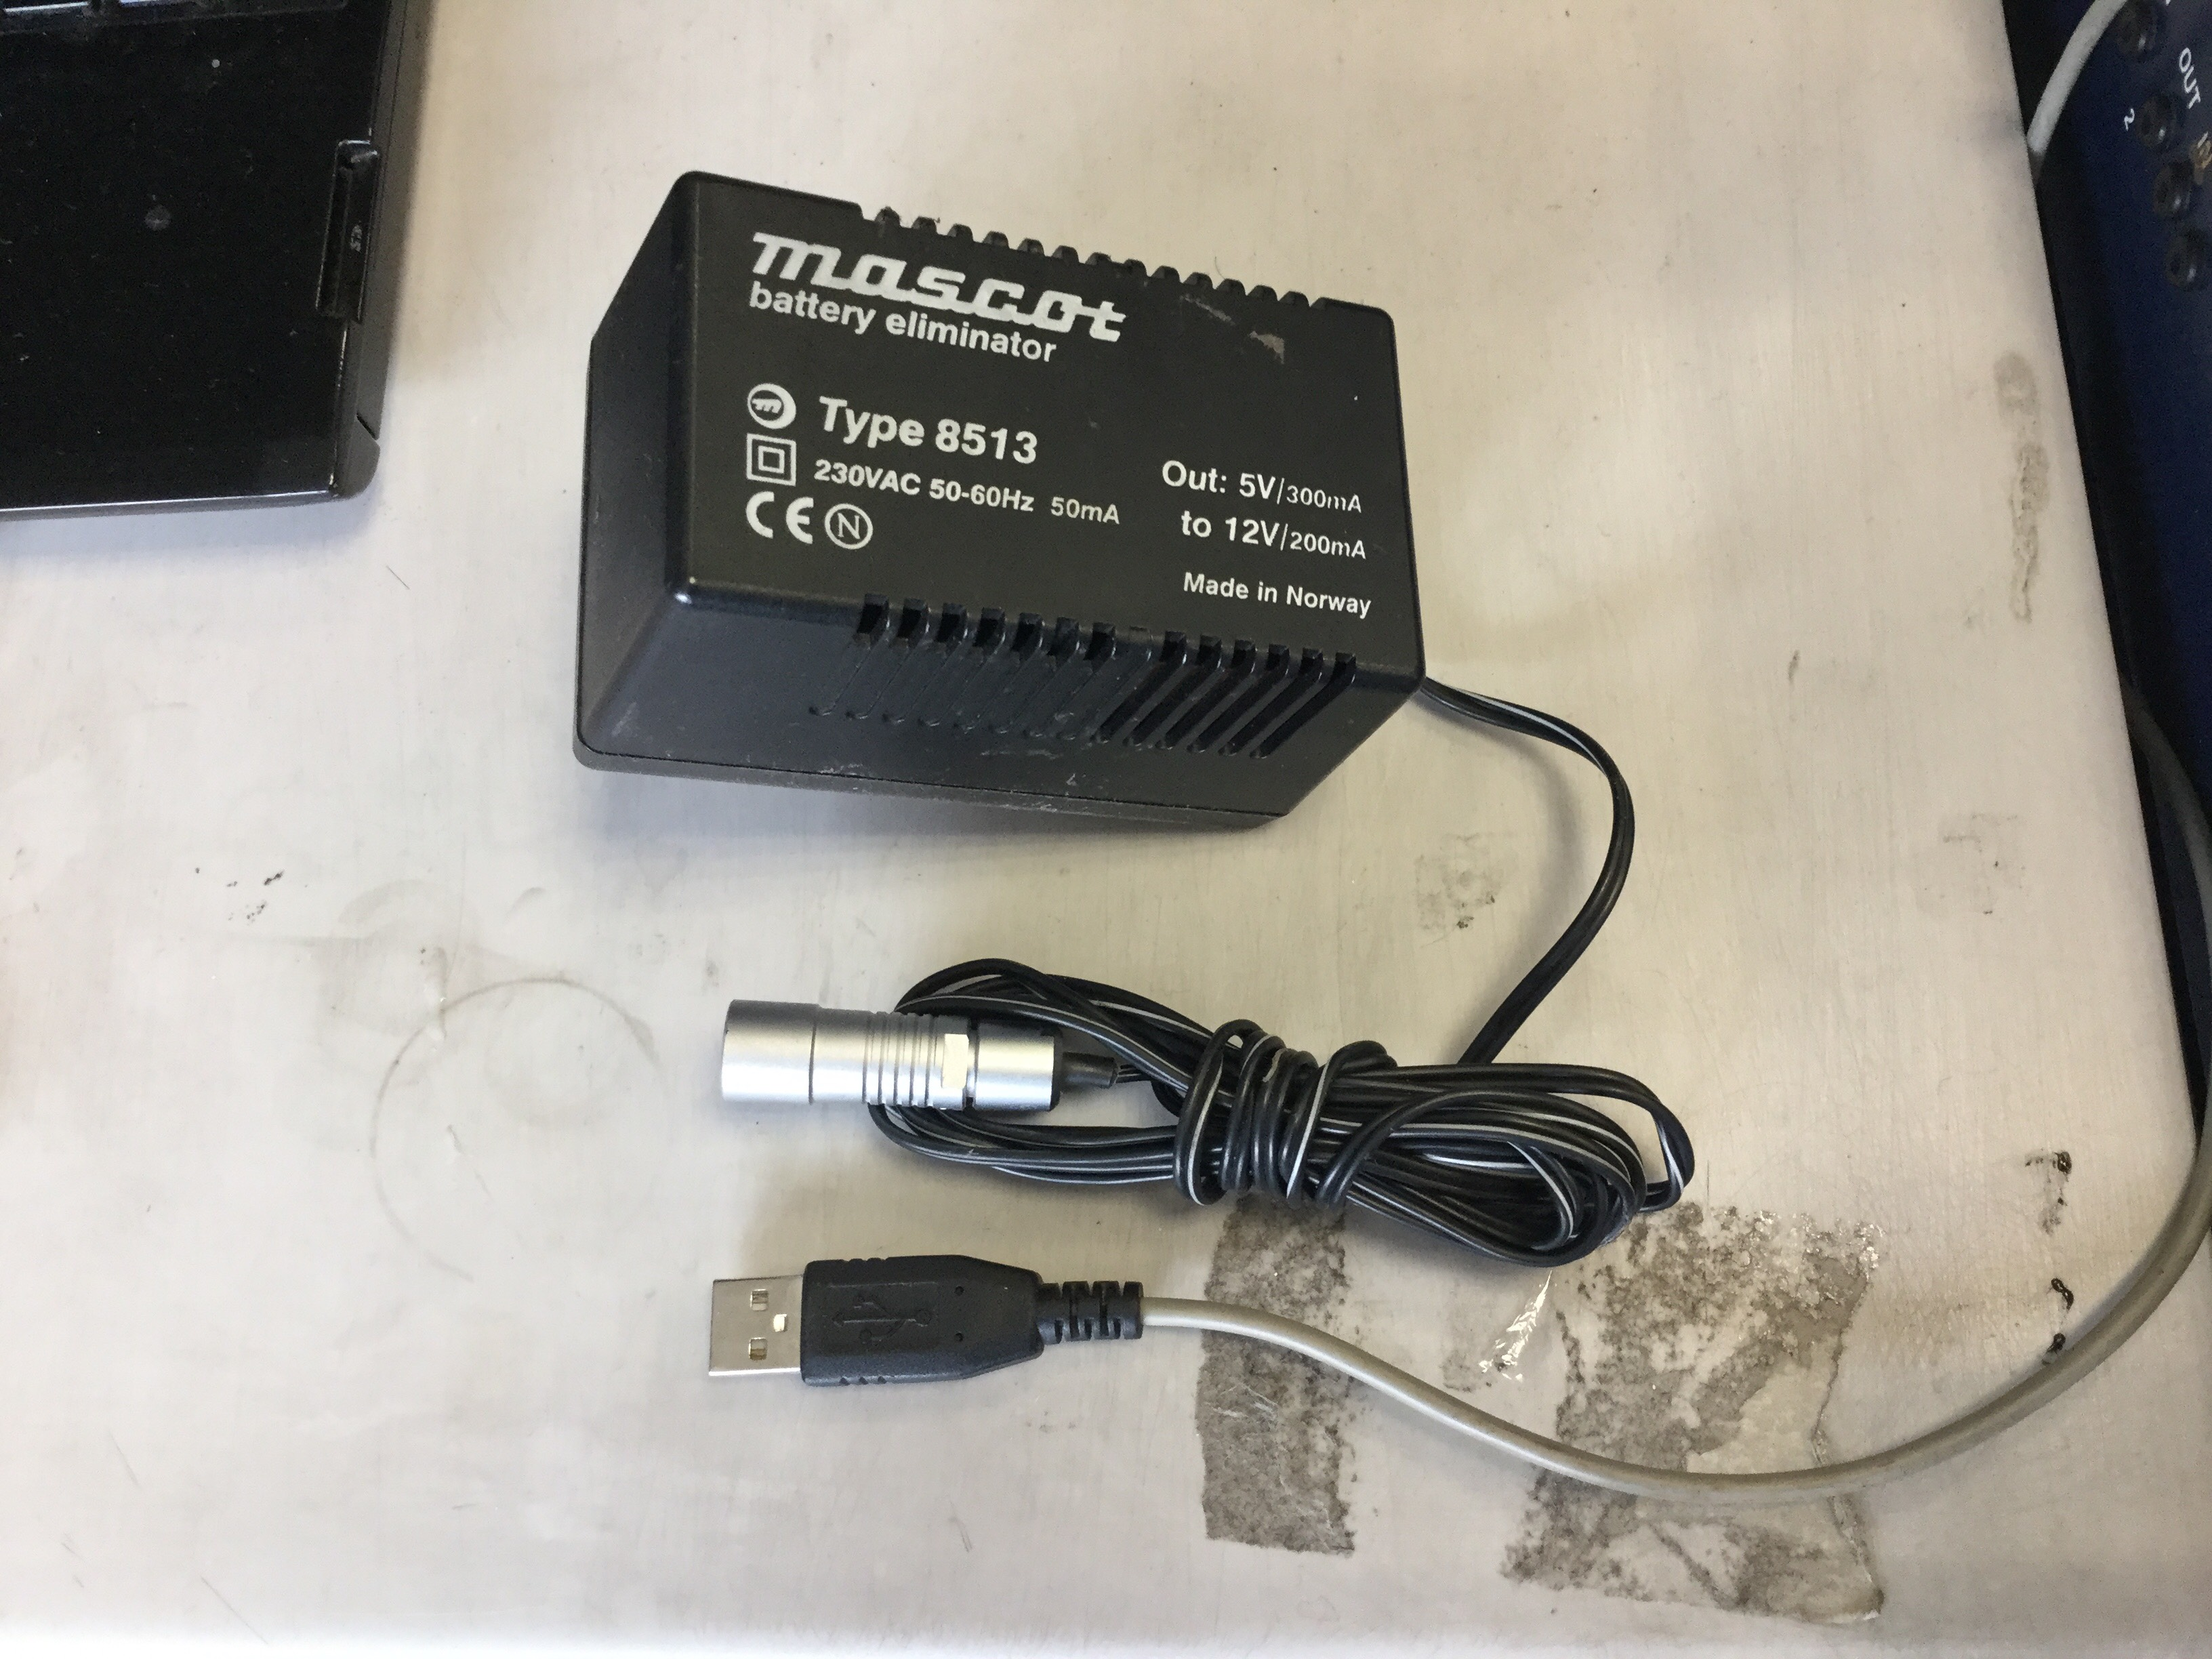
\includegraphics[width=0.5\linewidth]{Figures/motorCircuit}
		\caption{Sistema de alimentaci\'on original del agitador y el nuevo.}
	\end{figure}
	
	\section{Programa de control}
	El calorímetro cuenta con un programa de control con el nombre de Digitam. Este software se encuentra instalado en el computador que fue importado con el equipo, sin embargo, al momento de conectar el computador, no fue posible iniciar el sistema operativo. Usando un cable SATA-USB, se accedió al disco duro y se realizó una copia del mismo. Una aplicación de MS-DOS con el nombre de Digitam 3 se encontró en el mismo y se ejecutó en una maquina virtual con Windows XP y se logrando as\'i la comunicación con el calorímetro (\autoref{fig: digitam3}). Sin embargo, esta aplicaci\'on se ejecuta en la consola de Windows, por lo cual carece de interfaz gr\'afica y el uso del cursor es limitado. En el \'ultimo mes se identific\'o otro software el cual \'i presenta interfaz gr\'afica y hace la interacci\'on el usuario mucho m\'as c\'omoda \autoref{fig: digitam4}.
	\begin{figure}[h]
		\centering
		\begin{subfigure}{0.45\linewidth}
			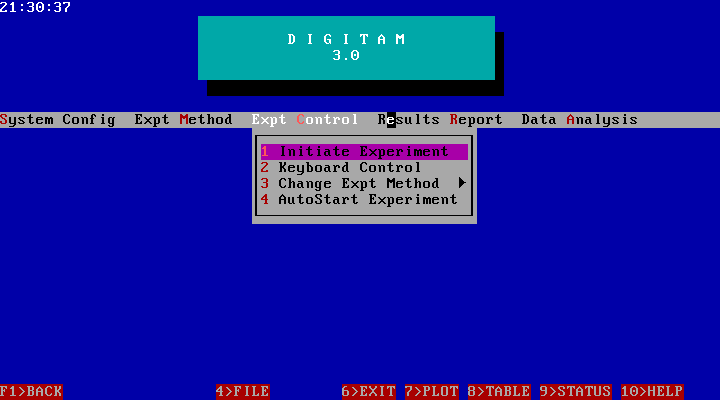
\includegraphics[width=\linewidth]{Figures/digitam}
			\caption{Digitam 3.0}
			\label{fig: digitam3}
		\end{subfigure}
		\begin{subfigure}{0.54\linewidth}
			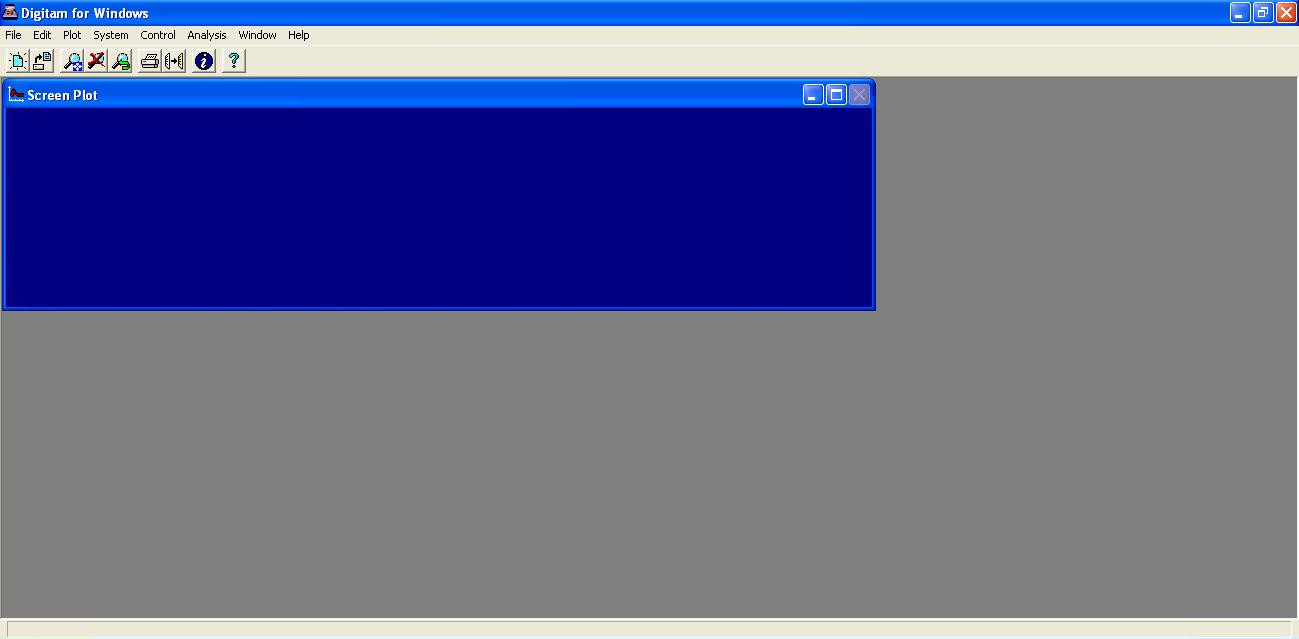
\includegraphics[width=\linewidth]{Figures/digitamView}
			\caption{Digitam 4.0}
			\label{fig: digitam4}
		\end{subfigure}
		\caption{Programas disponibles uso del calor\'imetro con Windows.}
	\end{figure}
	
	\subsection{Configuración del equipo}
	El programa depende de dos directorios en donde guarda los archivos que contienen c\'omo realizar un experimento (m\'etodos) y los resultados. Estos directorios se deben configurar cuando se instala el programa por primera vez y se encuentran en el men\'u principal de Digitam 4 en \texttt{File > Preferences}. En la ventana emergente se debe configurar la ubicaci\'on de los directorios (\texttt{Default results directory} y \texttt{Default method directory}), pues es posible que al iniciar el programa estos no existan por lo cual no sea posible continuar con las siguientes secciones.
	
	\subsection{Creación de un método experimental}
	Como fue mencionado anteriormente, el m\'etodo contiene la informaci\'on de qu\'e medir, con qu\'e frecuencia, si se desea inyectar un volumen determinado, realizar el experimento m\'ultiples veces, etc. Para crear un m\'etodo se debe seleccionar \texttt{File > New Method} o si se desea editar uno previo: \texttt{File > Open > Method}. En este punto se debe seleccionar como dividir el experimento, cada parte puede tener hasta cuatro secciones, como es el caso de las opciones 5 \'o 6. Adem\'as, se pueden concatenar hasta 3 partes seguidas, como se muestran en la \autoref{fig: methodCreation}.
	
	Posteriormente, se deben definir las condiciones que determinan un cambio de secci\'on en un una misma parte del m\'etodo. En el caso de \autoref{fig: methodSectionChange} para la tercera parte del experimento, en la secci\'on \texttt{Main}, se define la duraci\'on de este como 60 minutos, en el caso de usar las condiciones de estabilidad se debe expandir la opci\'on de \texttt{Section change condition} en el panel superior izquierdo, y definir las condiciones en \texttt{Signal conditions}.
	\begin{figure}[h]
		\centering
		\begin{subfigure}{0.45\linewidth}
			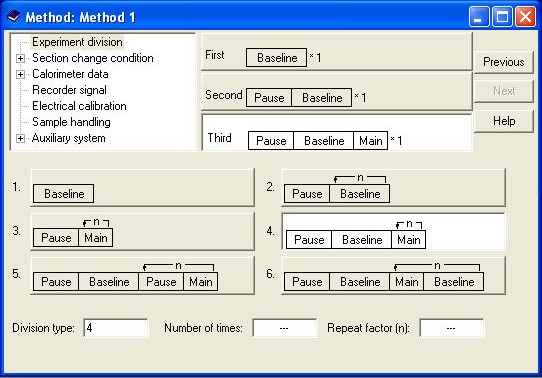
\includegraphics[width=\linewidth]{Figures/digitamMethod}
			\caption{Definici\'on de las partes y secciones de un m\'etodo.}
			\label{fig: methodCreation}
		\end{subfigure}
		\begin{subfigure}{0.45\linewidth}
			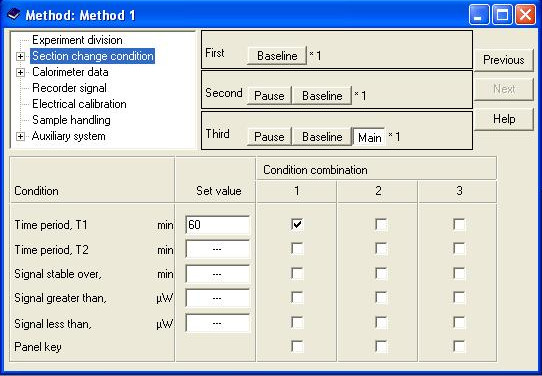
\includegraphics[width=\linewidth]{Figures/digitamMethod2}
			\caption{Configuraci\'on de las condiciones para cambiar de secci\'on.}
			\label{fig: methodSectionChange}
		\end{subfigure}
		\caption{Paneles de creaci\'on y modificaci\'on de un m\'etodo, configuraci\'on del mismo.}
		\label{fig: methodPanel}
	\end{figure}
	
	En \texttt{Calorimeter data} se escoge la frecuencia con la que se muestrea la se\~nal del calor\'imetro, si se quiere promediar la se\~nal a lo largo de cierta cantidad de tiempo, si se quiere filtrar digitalmente (usando las propiedades en \texttt{System > Calorimeter signal > Digital filter}) y si se quiere guardar la se\~nal din\'amicamente corregida. Al igual que en la \autoref{fig: methodSectionChange}, esta configuraci\'on es independiente para cada secci\'on del experimento. Por ejemplo, se puede medir la se\~nal de la primera parte en la secci\'on de \texttt{Baseline} cada segundo sin filtrar la se\~nal (\texttt{raw}), en la segunda parte, en \texttt{Pause} se puede medir la se\~nal corregida y en \texttt{Baseline} medir la potencia pero ahora cada 10 segundos.
	
	Las calibraciones el\'ectricas se configuran en \texttt{Electrical calibration} en el mismo panel de la \autoref{fig: methodPanel}. En ella se debe seleccionar el tipo (\texttt{D} para din\'amica y \texttt{S} para est\'atica), la potencia, que debe ser del mismo valor del amplificador del canal en el calor\'imetro (300 $\mu$W en el caso de la \autoref{fig: instalationMultiple}) \cite{Suurkuusk}, el tiempo, el cual se debe configurar \'unicamente para el caso de una calibraci\'on est\'atica y se recomienda que sea superior a 30 minutos \cite{Suurkuusk}. En general, el lado de la calibraci\'on es: \texttt{A} para la muestra y \texttt{B} para la celda de referencia \cite{Suurkuusk}, y la resistencia interna, que en el caso de los cilindros usados siempre es permanente \texttt{P}.
	
	La configuraci\'on de los vol\'umenes de inyecci\'on y los tiempos desde el programa, para el caso de titulaciones calorimétricas se describen en la \autoref{ssec: jeringa}. Una vez configurado el método, se debe guardar seleccionando \texttt{File > Save method}.
	
	\subsection{Control del experimento}
	Una vez se ha guardado el experimento, y se desea ejecutar el mismo, se accede al panel de comienzo del experimento. En \'el se debe seleccionar los nombres con los que se desean guardar los resultados, el m\'etodo experimental a usar, y el nombre del operario. Se debe verificar que la configuraci\'on de amplificaci\'on corresponde con la que tiene el canal en el calor\'imetro, y si se realizar\'an inyecciones en una titulaci\'on, el n\'umero del controlador de la jeringa, que en este caso corresponde con \texttt{1}.
	
	\subsection{Configuración de la gráfica}
	Digitam 4 ofrece la posibilidad de graficar los resultados en tiempo real, para esto se debe configurar la gr\'afica. Al acceder a \texttt{Plot > Define Screen Plot} se escribe el nombre de los resultados a graficar, se definen las escalas de la gr\'afica, y el tipo de datos a usar (corregidos, filtrados u originales). Adicionalmente se puede optimizar el \'area de la gr\'afica para que muestre la totalidad de los datos, oprimiendo \texttt{Plot > Scale to Show All}.
	
	\subsection{Extracci\'on los resultados}
	Finalmente, y con el objetivo de exportar los resultados se debe oprimir en el men\'u superior \texttt{File > Open > Results file} y seleccionar el archivo de resultados que se desea abrir. Posteriormente, se debe navegar sobre el diagrama de \'arbol en donde se muestran los par\'ametros de cada secci\'on del m\'etodo experimental. En particular, para obtener los datos registrados por el calor\'imetro se selecciona \texttt{Numeric data} y luego en \texttt{Tabulated}. Luego, se debe ir al men\'u superior y oprimir \texttt{File > Export}, en el dialogo \texttt{Results Report} seleccionar \texttt{Generate numeric data report for table import}, seleccionar las columnas a incluir y elegir el nombre del archivo de salida.
	
	El archivo de salida puede ser le\'ido en Excel, importando los datos con la opci\'on \texttt{Desde texto} en la ventana \texttt{Datos}. La informaci\'on del calor\'imetro se encuentra tabulada con \texttt{Tabs} como delimitador de cada valor, y en la opci\'on de \texttt{origen del archivo} se puede seleccionar \texttt{Wndows ANSI}. Al finalizar este procedimiento los datos pueden ser visualizados en la hoja de c\'alculo.
	
	\section{Efecto del agitador en las lecturas}
	Para comprobar el efecto del agitador en la potencia registrada por el equipo se llevaron a cabo 6 ciclos de conexión-desconexión con 15 minutos entre cada perturbación al sistema, horas después de haber realizado una calibración estática. Las diferencias de potencia generadas entre cada conexión (izquierda) y desconexión (derecha) se muestran en la \autoref{tb: connection}, y en la \autoref{fig: connection}, donde se observan como aumentos y descensos súbitos en la potencia registrada.
	\begin{table}[h]
		\centering
		\caption{Efectos inmediatos de conectar y desconectar el agitador.}
		\begin{tabular}{cc|l|cc|l}
			\hline
			\textbf{Antes ($\mu$W)} & \textbf{Después ($\mu$W)} &  $\Delta$ ($\mu$W) &  \textbf{Antes ($\mu$W)} & \textbf{Después ($\mu$W)} &  $\Delta$ ($\mu$W) \\
			\hline
			-7,58 &  -5.5 & 2,08 & -5,84 & -7,78 & -1,94 \\
			-6,12 & -3.78 & 2,34 & -5,12 & -7,04 & -1,92 \\
			-5,04 & -2.76 & 2,28 & -4,17 & -6,48 & -2,31 \\
			-5,43 & -3.21 & 2,22 & -5,22 & -7,31 & -2,09 \\
			-6,65 & -4.72 & 1,93 & -6,71 & -8,54 & -1,83 \\
			-7,75 & -5.84 & 1,91 & -8,35 & -9,93 & -1,58 \\
			\hline
			 & \textbf{promedio} ($\mu$W) & 2,1 $\pm$ 0,2 & & & -1,9 $\pm$ 0,2 \\
			\hline
		\end{tabular}
		\label{tb: connection}
	\end{table}

	A partir de los datos de la \autoref{tb: connection} fue posible establecer que el efecto de prender y apagar el agitador es de aproximadamente 2 $\mu$W, siendo un aumento en el caso de conexión y una disminución al desconectarlo. Lo anterior tiene sentido, pues el agitador realiza trabajo sobre la solución, que al encontrarse en un sistema isotérmico la energía se transmite la energ\'ia en forma de calor, y de forma diferencial será registrado como un aumento de potencia en el calorímetro. La \autoref{fig: connection} por su lado, muestra que este efecto es local en el tiempo y que el sistema tiende a equilibrarse nuevamente al valor de la línea base. Esto se infiere pues el sistema luego de registrar el aumento súbito experimenta una disminución de la potencia lenta, lo contrario ocurre con la desconexión, por lo cual el sistema tiende a retomar el equilibrio dado por la curva naranja, la cual se obtiene realizando mínimos cuadrados con los datos sobre un polinomio de grado 2.
	\begin{figure}[h]
		\centering
		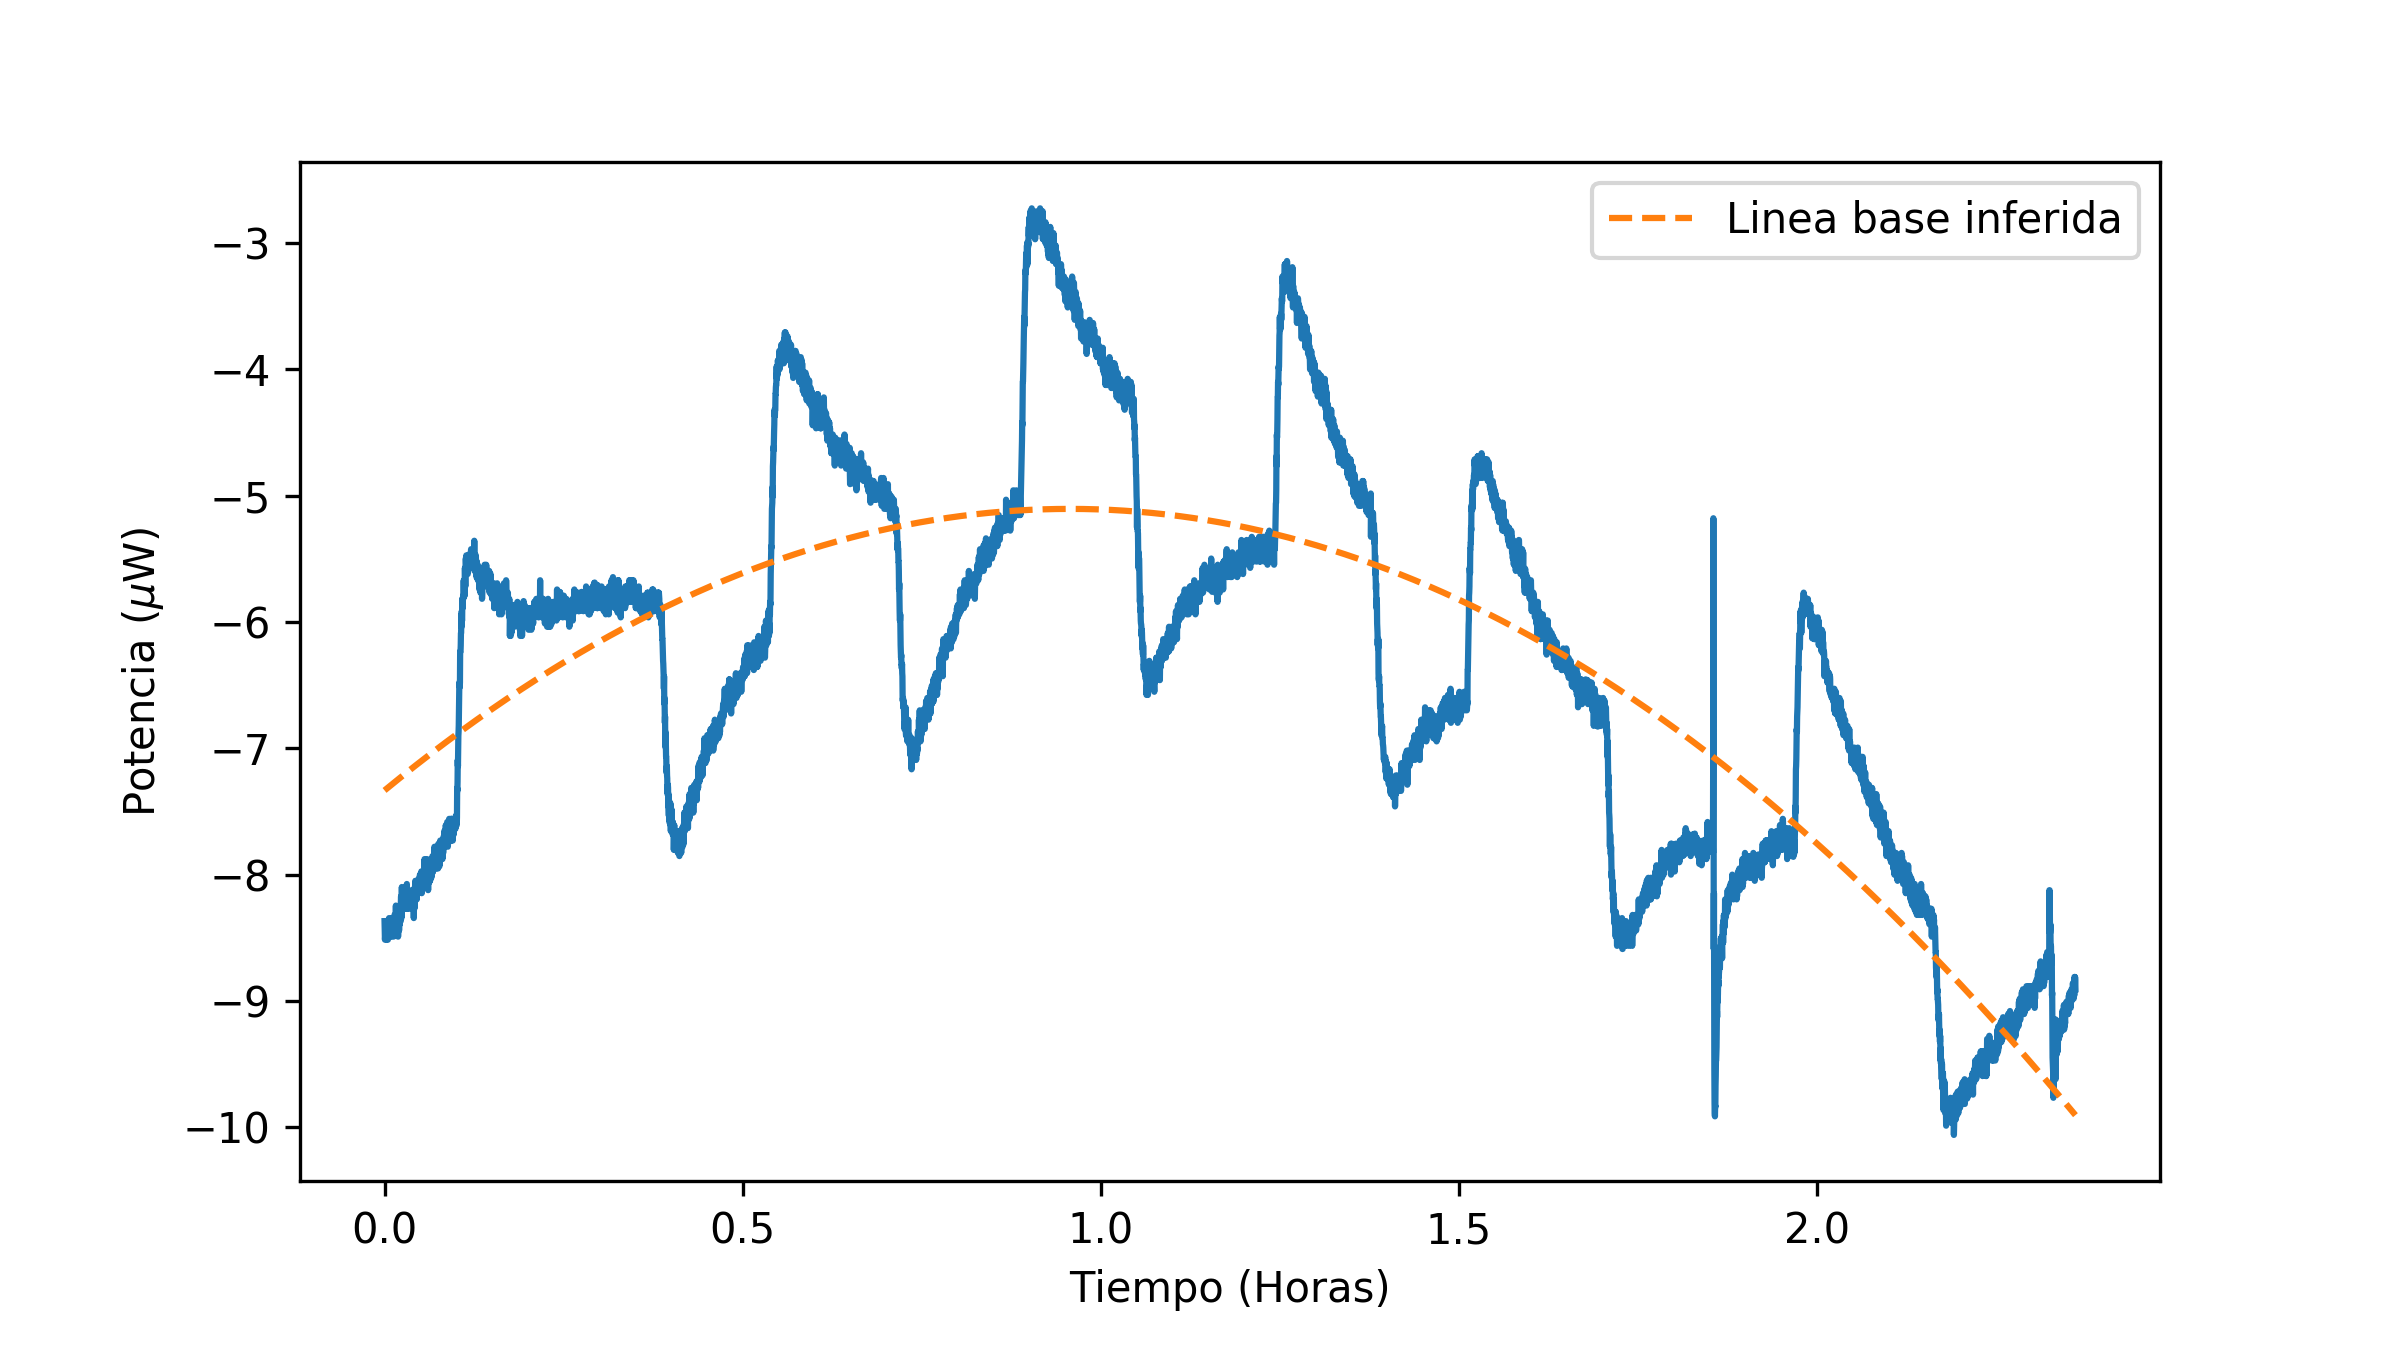
\includegraphics[width=\linewidth]{../Data/Baselines/motor}
		\caption{Conexiones y desconexiones del agitador que perturban la línea base, sin embargo, lentamente el equipo vuelve al equilibrio.}
		\label{fig: connection}
	\end{figure}	
% !TeX spellcheck = es_ES
% Chapter 1

%\chapter{Chapter Title Here} % Main chapter title
%
%\label{Chapter1} % For referencing the chapter elsewhere, use \ref{Chapter1} 

%----------------------------------------------------------------------------------------

% Define some commands to keep the formatting separated from the content 
%\newcommand{\tabhead}[1]{\textbf{#1}}
%\newcommand{\code}[1]{\texttt{#1}}
%\newcommand{\file}[1]{\texttt{\bfseries#1}}
%\newcommand{\option}[1]{\texttt{\itshape#1}}

%----------------------------------------------------------------------------------------

\chapter{Control de la temperatura}\label{ch: thermal}
	El sistema cuenta con dos calentadores de precisión al interior del baño termostatado de 25 litros. Estos calentadores junto con el ba\~no externo determinan la temperatura de trabajo del equipo. El ba\~no externo se usa con el objetivo de mantener siempre activos los calentadores internos en alg\'un nivel de potencia intermedio, pues el ba\~no externo, al tener una temperatura inferior agrega una carga permanente a los calentadores internos \cite{Suurkuusk}. Para monitorear la temperatura del ba\~no el calor\'imetro, cuenta con dos termistores, el primero para trabajar a temperaturas inferiores a 50 \grad{} y el segundo para temperaturas superiores a este valor. La se\~nal generada por uno de estos termistores se compara con un valor de resistencia definido por el usuario. La resistencia, y por ende la temperatura del equipo, se fijan usando cuatro resistencias de década, esto es que cada resistencia es una potencia de 10 menor que la anterior. Estas se encuentran en la parte inferior del calor\'imetro, en la \autoref{fig: decadeResistors} corresponden con A, B, C, y D, de esta manera se pueden realizar experimentos a temperaturas en el rango de 5 a 80 \grad{}. El diagrama del sistema de control t\'ermico del calor\'imetro se muestra en el \autoref{anx: imagenes} como \autoref{fig: controlTermico}.
	
	\begin{figure}[h]
		\centering
		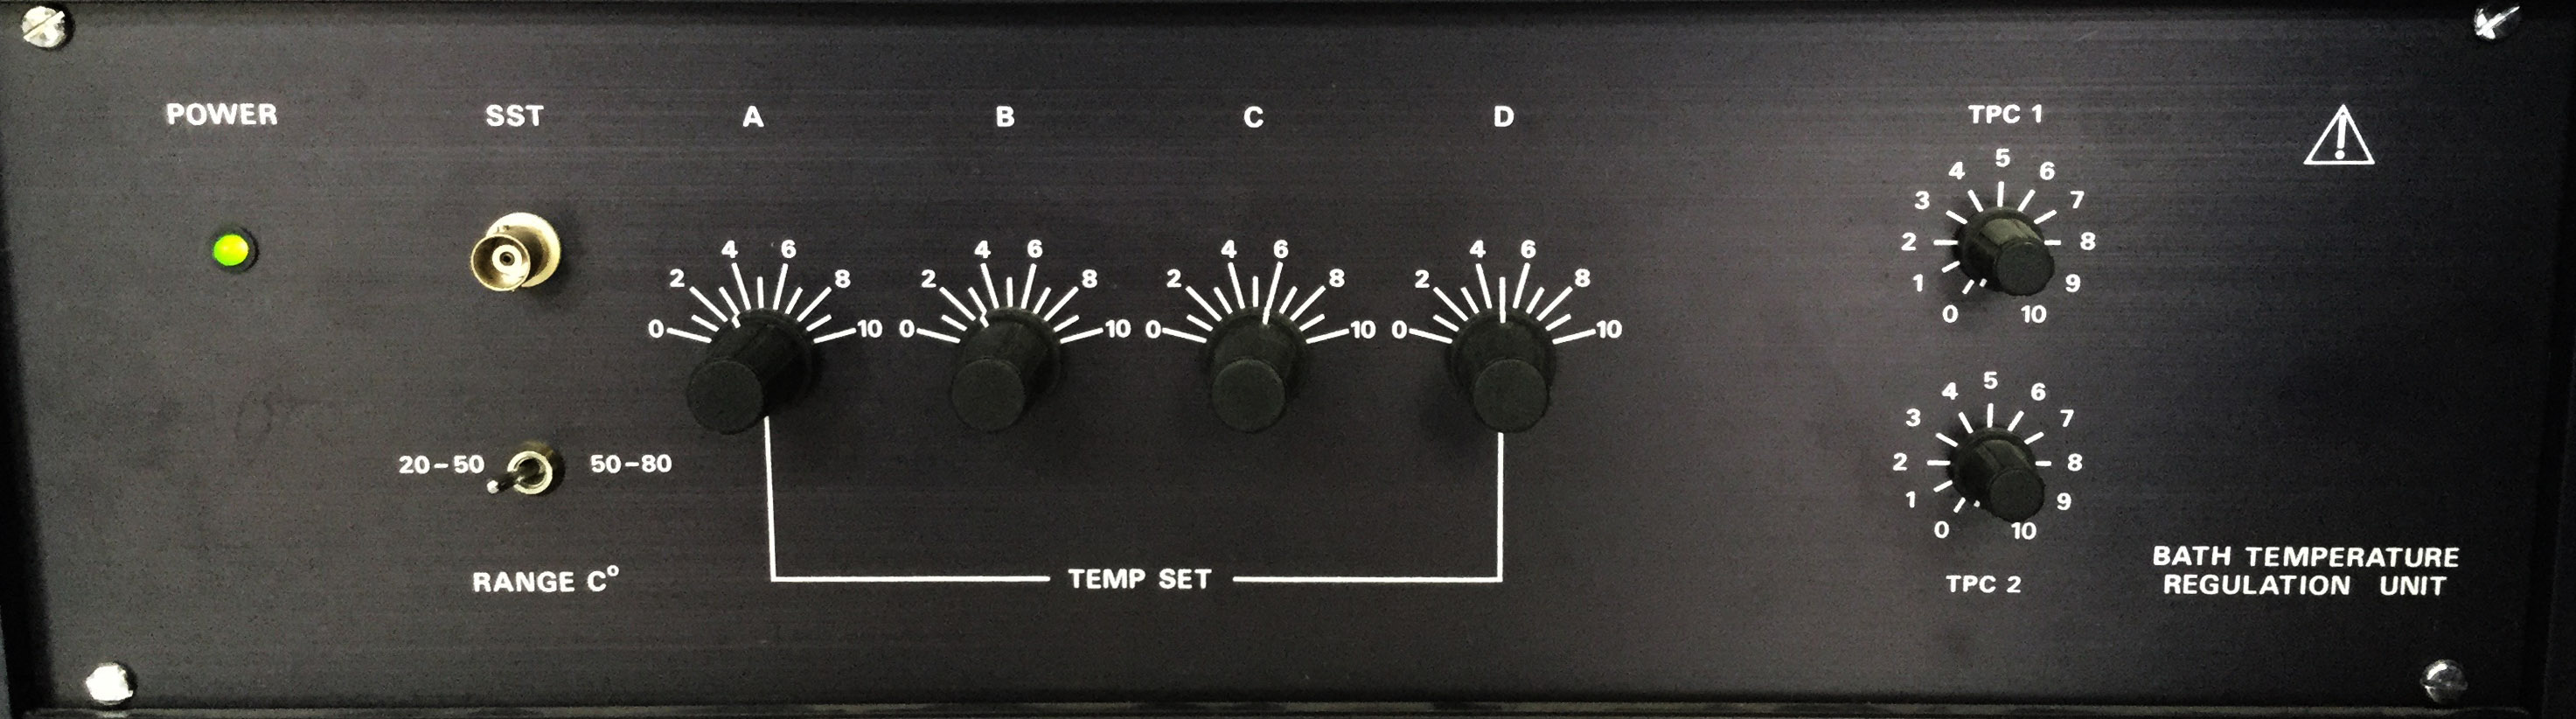
\includegraphics[width=0.7\linewidth]{Figures/decadeResistors}
		\caption{Resistencias de década que controlan la temperatura.}
		\label{fig: decadeResistors}
	\end{figure}
	
	Para determinar la equivalencia entre resistencia y temperatura, el calorímetro cuenta con una tabla que relaciona dichos valores junto con la temperatura del ba\~no externo que dan lugar a una temperatura constante en el ba\~no interno. Dicha tabla se muestra en el \autoref{anx: imagenes} como \autoref{fig: temperatureTable}, sin embargo, el uso de esa tabla est\'a limitado a temperaturas ambiente superiores a 20 \grad{} por lo cual, en el caso particular de Bogot\'a, rara vez se cumplen. Lo anterior es relevante dado que la resistencia el\'ectrica depende de la temperatura, en el caso de materiales met\'alicos la resistencia aumenta con la temperatura, y para semiconductores se tiene el efecto contrario \cite{simon2013oxford}.
	
	Una vez realizadas las conexiones el\'ectricas del calor\'imetro para su funcionamiento a 110 VAC, y antes de realizar una calibraci\'on qu\'imica, fue necesario estabilizar el equipo a una temperatura de 25 \grad{}, puesto que el objetivo de la calibraci\'on qu\'imica es contrastar los datos obtenidos con el calor\'imetro respecto a los reportados en la literatura, los cuales por convenci\'on se reportan a estas condiciones. Para alcanzar esta temperatura se probó con las condiciones reportadas en la \autoref{fig: temperatureTable}, en donde los valores de cada resistencia de década se muestra a continuación. 
	\begin{table}[h]
		\centering
		\caption{Valores de las resistencias de década, para una temperatura de 25 \grad{}, seg\'un calibración original del calorímetro.}
		\begin{tabular}{r|cccc|l}
			\hline
			\textbf{Baño interno (\grad{})} & A ($10^4$ $\Omega$) & B ($10^3$ $\Omega$) & C ($10^2$ $\Omega$) & D ($10^1$ $\Omega$) & \textbf{Baño externo (\grad{})} \\
			\hline
			25,0 & 3 & 2 & 4 & 9 & 22,0 \\
			\hline
		\end{tabular}
		\label{tb: decadeResistorsBefore}
	\end{table}
	
	La temperatura del equipo fue monitoreada por cuatro días, con al menos un registro diario, los resultados se muestran en la \autoref{tb: temperatureRegister}. En ella se puede observar que cuando inicialmente se creía que la temperatura del baño estaba cerca de estabilizarse a 25 \grad{}, en realidad estaba en aumento, y cuando se creía que finalmente el calorímetro se había estabilizado en 26,86 \grad{} el sistema se encontraba oscilando, como lo muestra la última temperatura registrada.
	
	\begin{table}[h]
		\centering
		\caption{Registro de temperaturas del baño interno en el tiempo para la configuración recomendada por la calibración en la \autoref{fig: temperatureTable}.}
		\begin{tabular}{r|c}
			\hline
			\textbf{Fecha (DD/MM HH:MM)} & \textbf{Temperatura (\grad{})} \\
			\hline
			07/09 11:13 & 25,14 \\
			07/09 11:50 & 25,19 \\
			10/09 09:43 & 26,64 \\
			11/09 09:22 & 26,86 \\
			11/09 10:00 & 26,86 \\
			12/09 08:30 & 26,86 \\
			12/09 10:30 & 26,86 \\
			12/09 15:48 & 26,64 \\
			\hline
		\end{tabular}
		\label{tb: temperatureRegister}
	\end{table}
	
	Sin embargo, esta no fue la única configuración probada, pues también se trató de estabilizar el equipo usando: 2977 (ABCD), que dio lugar a las siguientes temperaturas de baño interno 25,44 \grad{}, y 28,38 \grad{} luego de 5 días. De manera similar se probaron 3000, 3021, 3040, 3100, 3121, 3140, 3160 ninguna de las cuales presentó una temperatura estable. Debido a la dificultad de estabilizar el equipo a una temperatura determinada, se decidió construir un sistema de monitoreo automatizado para facilitar esta tarea, de esta manera se podría saber el histórico de una configuración, si el sistema está en calentamiento, estable, u oscilando.
	
	\section{Sistema de monitoreo}
	De todas las acciones que se hicieron a lo largo del proyecto, la estabilizaci\'on de la temperatura fue la que llev\'o m\'as tiempo. Esto, debido a que existen dos variables que determinan una temperatura en el calor\'imetro, por una parte la configuraci\'on de las resistencias de d\'ecada, y por otro el ba\~no externo, adem\'as se debe tener en cuenta el tiempo de estabilizaci\'on del calor\'imetro, el cual puede tomar cerca de 6 horas en completarse. Para monitorear el estado de la temperatura del ba\~no interno se construy\'o un circuito con tres sensores de temperatura, los sensores LM39 fueron elegidos debido a que presentan una respuesta lineal en voltaje, y tienen un rango de trabajo de 2 \grad{} a 120 \grad{} \cite{instruments1999lm35}. Cada uno de estos sensores fue conectado a tres cables como se muestra en la \autoref{fig: sensors}, y posteriormente fue cubierto con silicona y un cable termoencogible para aislar el sensor del agua. 	
	\begin{figure}[h]
		\centering
		\begin{subfigure}{0.75\textwidth}
			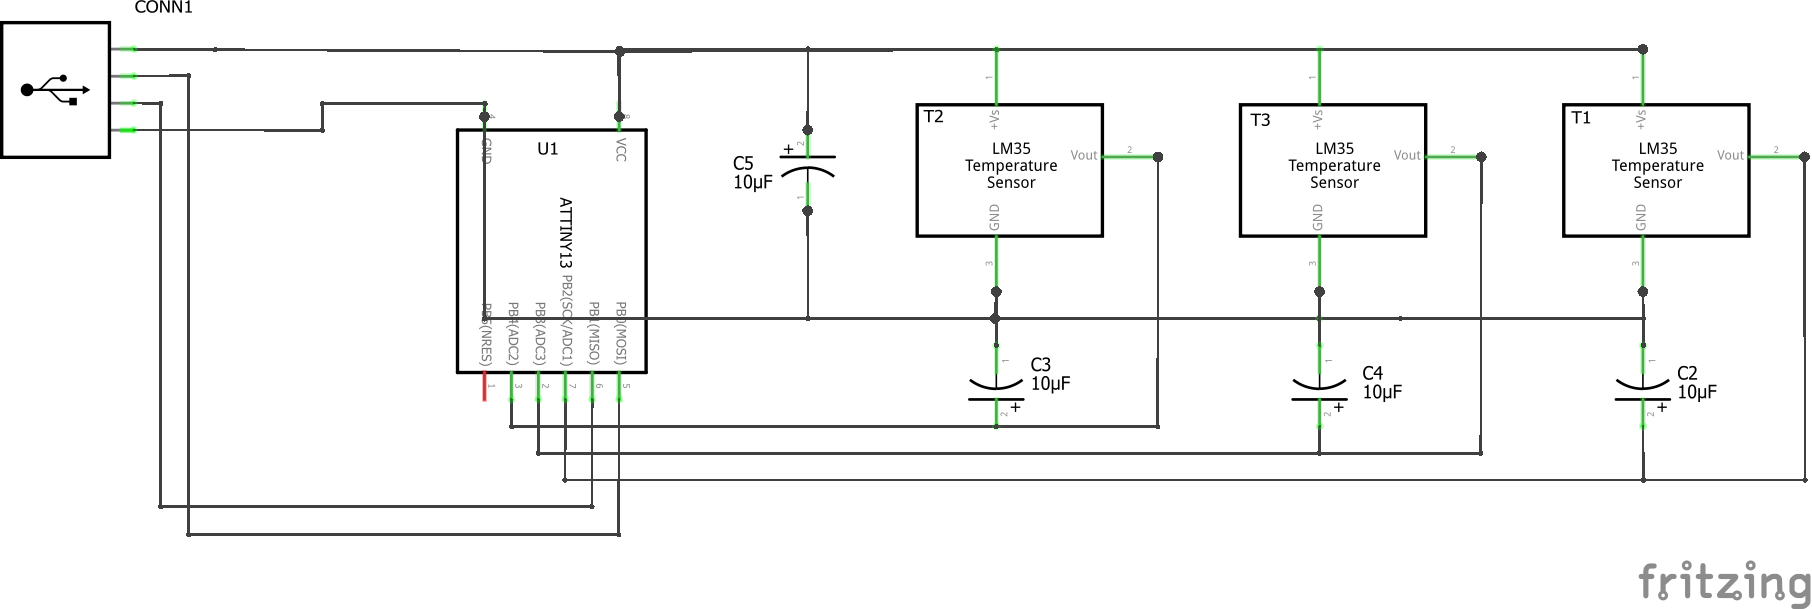
\includegraphics[width=\linewidth]{Figures/Sketch_schem}
			\caption{Conexi\'on al microcontrolador.}
			\label{fig: circuito}
		\end{subfigure}
		\begin{subfigure}{0.23\textwidth}
			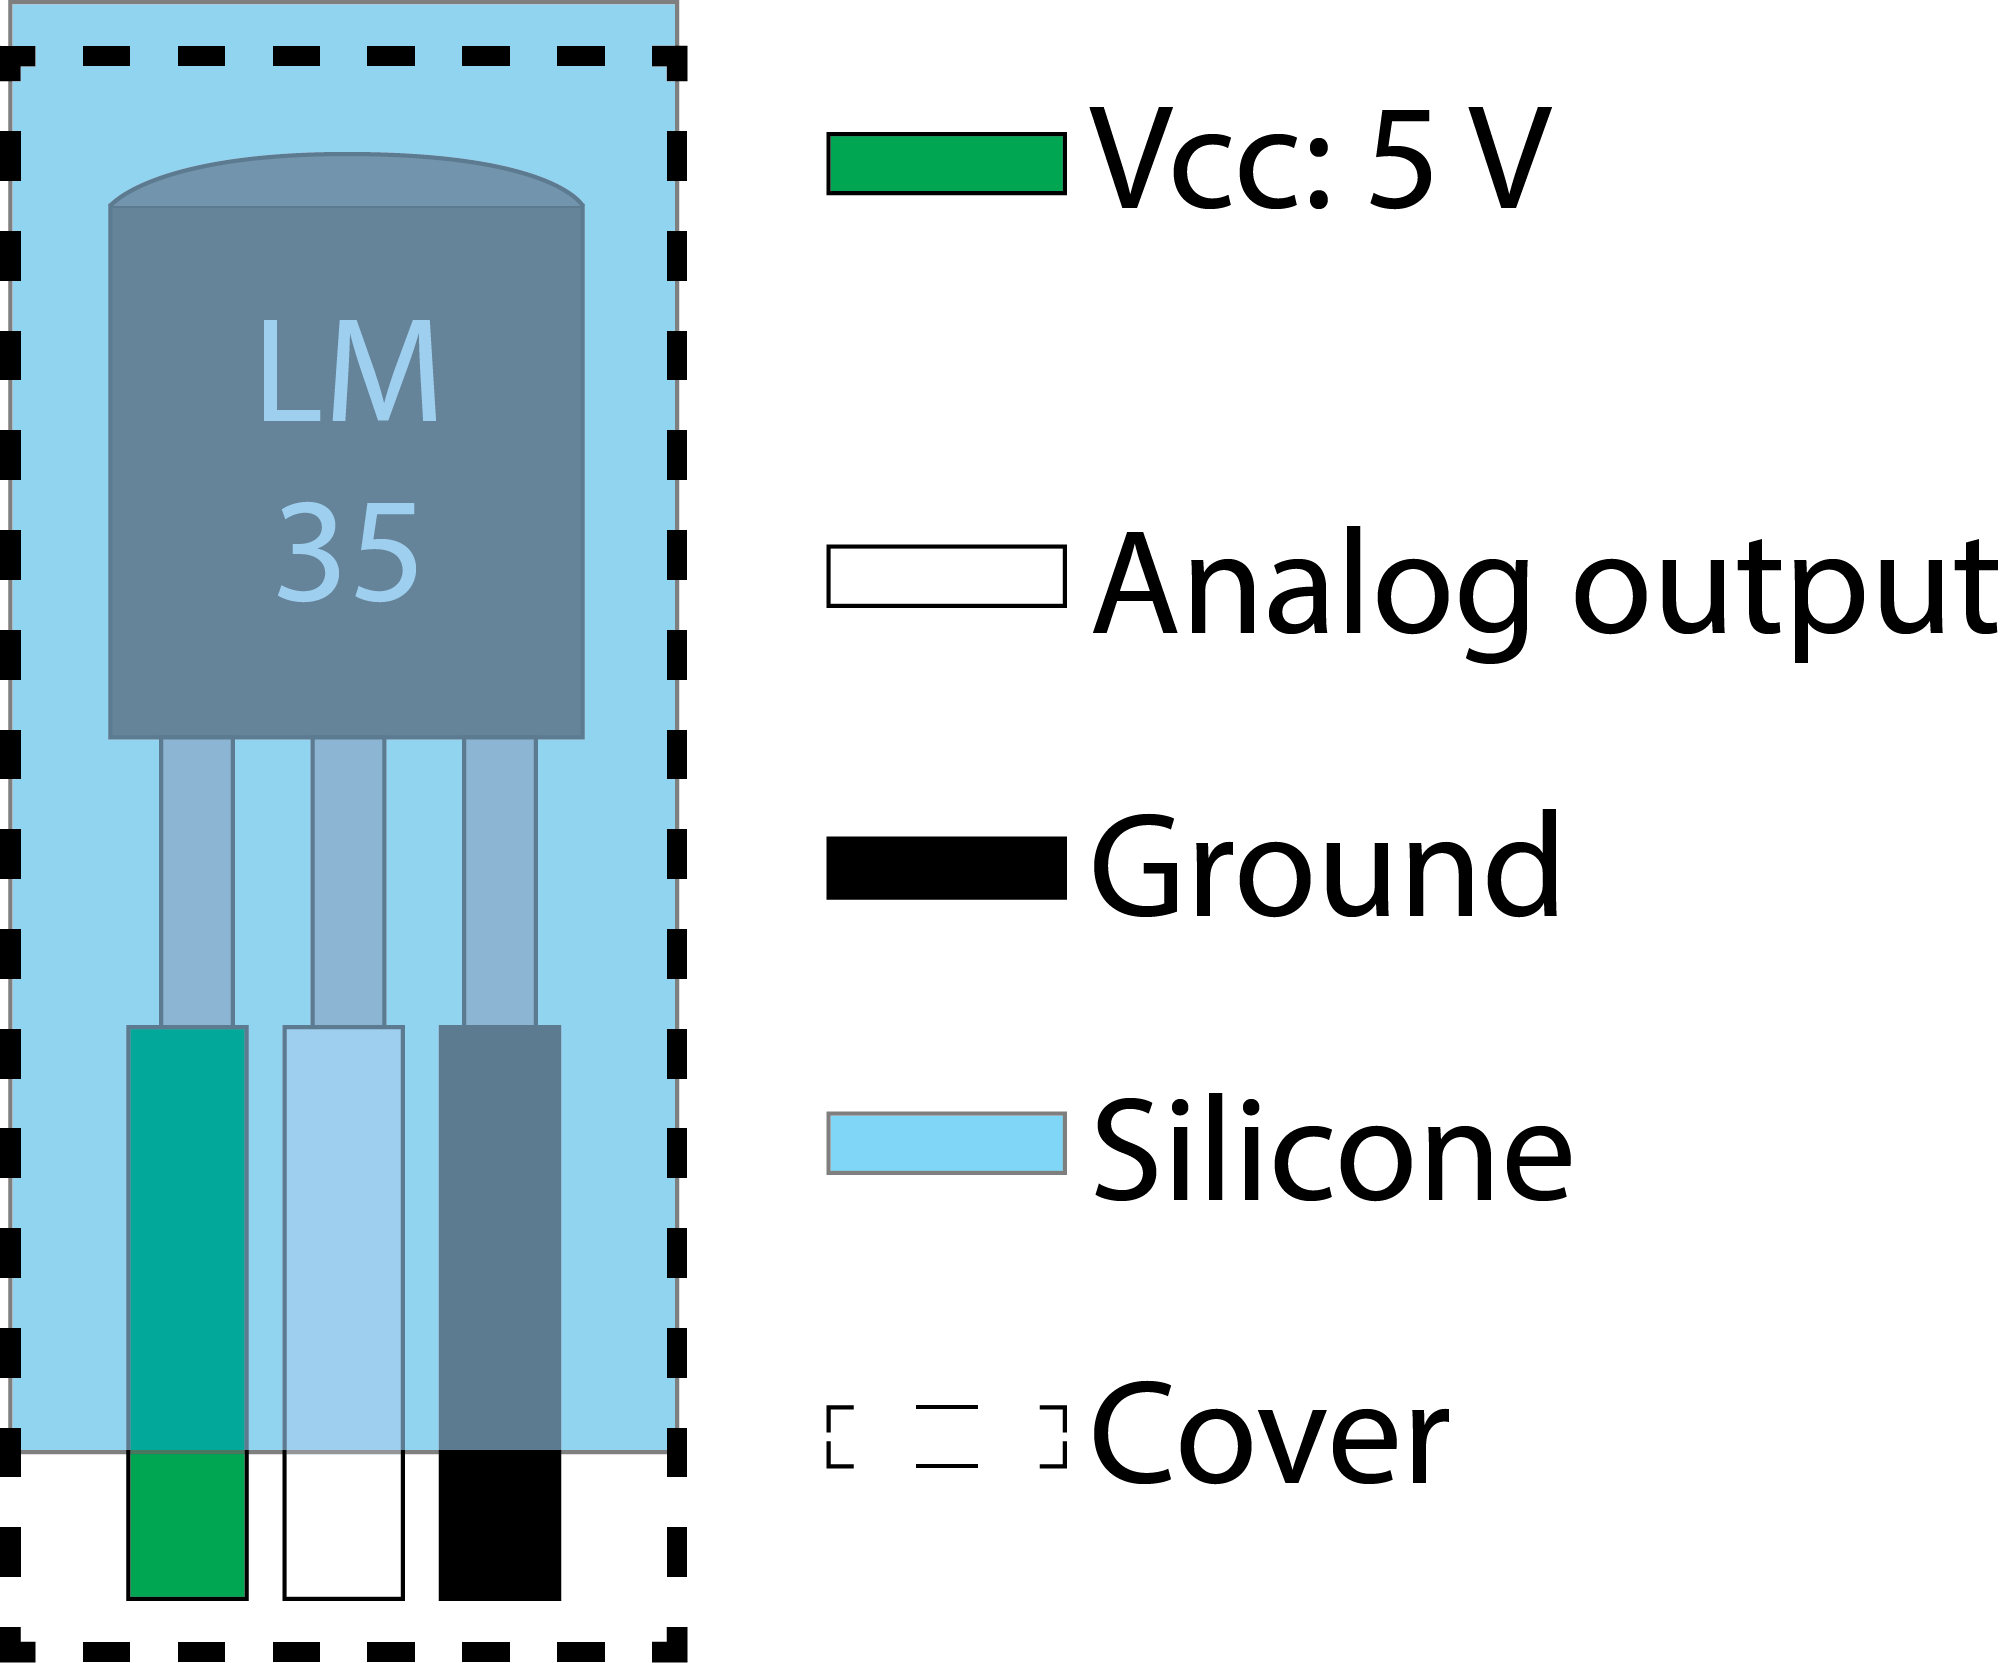
\includegraphics[width=\linewidth]{Figures/Sensor}
			\caption{Cableado del sensor LM35.}	
			\label{fig: sensors}
		\end{subfigure}
		\caption{Circuito del sistema de monitoreo de temperatura.}	
	\end{figure}

	Los sensores, uno para el baño interno, baño externo y temperatura ambiente, a su vez fueron conectados a un microcontrolador ATtiny 13 \cite{attiny13} (\autoref{fig: circuito}), el cual hace las veces de central de procesamiento que unifica las señales de los tres sensores y las envía a un computador usando el protocolo de comunicación UART (\textit{Universal Asynchronous Receiver-Transmitter} por sus siglas en inglés). Para convertir las señales de los sensores a un valor digital se usa el ADC (\textit{Analog to Digital Converter} por sus siglas en inglés) con el que cuenta el microcontrolador. El ADC compara el voltaje de la señal de entrada con un valor de referencia de voltaje y determina que fracción de voltaje corresponde la señal de entrada, este valor relativo ($k$) se encuentra entre 0 y 2$^{n}$ ($n$ es el número de bits del ADC), donde 0 implica un valor igual al de la tierra del circuito, y 2$^n$ tiene lugar cuando la señal de entrada tiene el mismo valor que el voltaje de referencia, los valores intermedios son lineales con los límites, de tal forma que es posible reconstruir el valor de la señal en voltios mediante la siguiente ecuación:
	\begin{equation}
		V = \left(\dfrac{k}{2^n}\right)V_{\text{ref}}
	\end{equation}
	
	En el caso del ATtiny 13, se cuenta con 10 bits en el ADC con cuatro canales, tres de los cuales son usados para los sensores. Como voltaje de referencia se usa un regulador interno del microcontrolador cuyo valor es 1,1 V \cite{attiny13}. Un voltaje de salida del sensor de 1,1 V en el sensor es cercano a 110 \grad{} y 0,0 V cercano a 0 \grad{} pues el fabricante asegura que por cada grado Celsius el voltaje de salida aumenta en 10 mV. El número de bits del ADC permite una resolución cercana a los 0.1 \grad{}, puesto que se tiene que 110 \grad{} pueden ser divididos en $2^{10} = 1024$ niveles distintos. Sin embargo, para lograr una resolución de 0.01 \grad{} se usó una técnica conocida como sobremuestreo \cite{grewal2006oversampling}. Esta técnica tiene sus orígenes en el teorema de Nyquist, el cual establece que para reconstruir una señal es necesario muestrear una señal con el doble de la frecuencia de la frecuencia máxima en la señal \cite{alexander2009fundamentals}. En el caso de la temperatura de los baños de agua y ambiente, se espera que la frecuencia máxima sea relativamente baja, del orden del tiempo de respuesta del sensor el cual es del orden de segundos. En particular se tiene que para $w$ bits adicionales en el ADC es necesario muestrear $4^w$ veces adicionales la señal. Dado que se tiene un rango cercano a los 100 grados y se quiere una resolución de 0,01 \grad{} es necesario diferenciar 10.000 niveles distintos de voltaje, lo cual implica al menos 14 bits ($2^{14}=$16.384), sin embargo, se eligen muestrear 4096 veces con frecuencia de 150 kHz, lo cual equivale a 16 bits en el ADC.
	
	Los sensores fueron calibrados usando el baño externo, y el termómetro de mercurio previamente usado en la verificación de la lectura de temperatura del sensor interno del calorímetro. Para esto se realizó una rampa de calentamiento discreta de 10 \grad{} hasta 50 \grad{} con pasos de 5 \grad{} y tiempos de estabilización de 20 minutos. Se escribió un algoritmo que calcula el valor promedio y desviación estándar de una lectura de voltaje para los intervalos estacionarios de la rampa. Este algoritmo realiza lo siguiente:
	\begin{enumerate}
		\item Para cada instante de tiempo considera el promedio de voltaje de los tres sensores.
		\item Saca el valor absoluto de la derivada de los datos en el tiempo.
		\item Aplica un filtro de medianas con kernel 507 sobre los datos anteriores (líneas continuas rojas en la \autoref{fig: calAlgorithm}).
		\item Los puntos con valores menores a 0,05 se les asigna el valor 0, para los otros valores se asigna 0,5 (lineas segmentadas en la \autoref{fig: calAlgorithm}).
		\item Se considera que los puntos donde el valor anterior corresponde a 0 son estables, sobre estos intervalos calcula el promedio y desviación estándar de cada sensor.
	\end{enumerate}
	
	\begin{figure}[h]
		\centering
		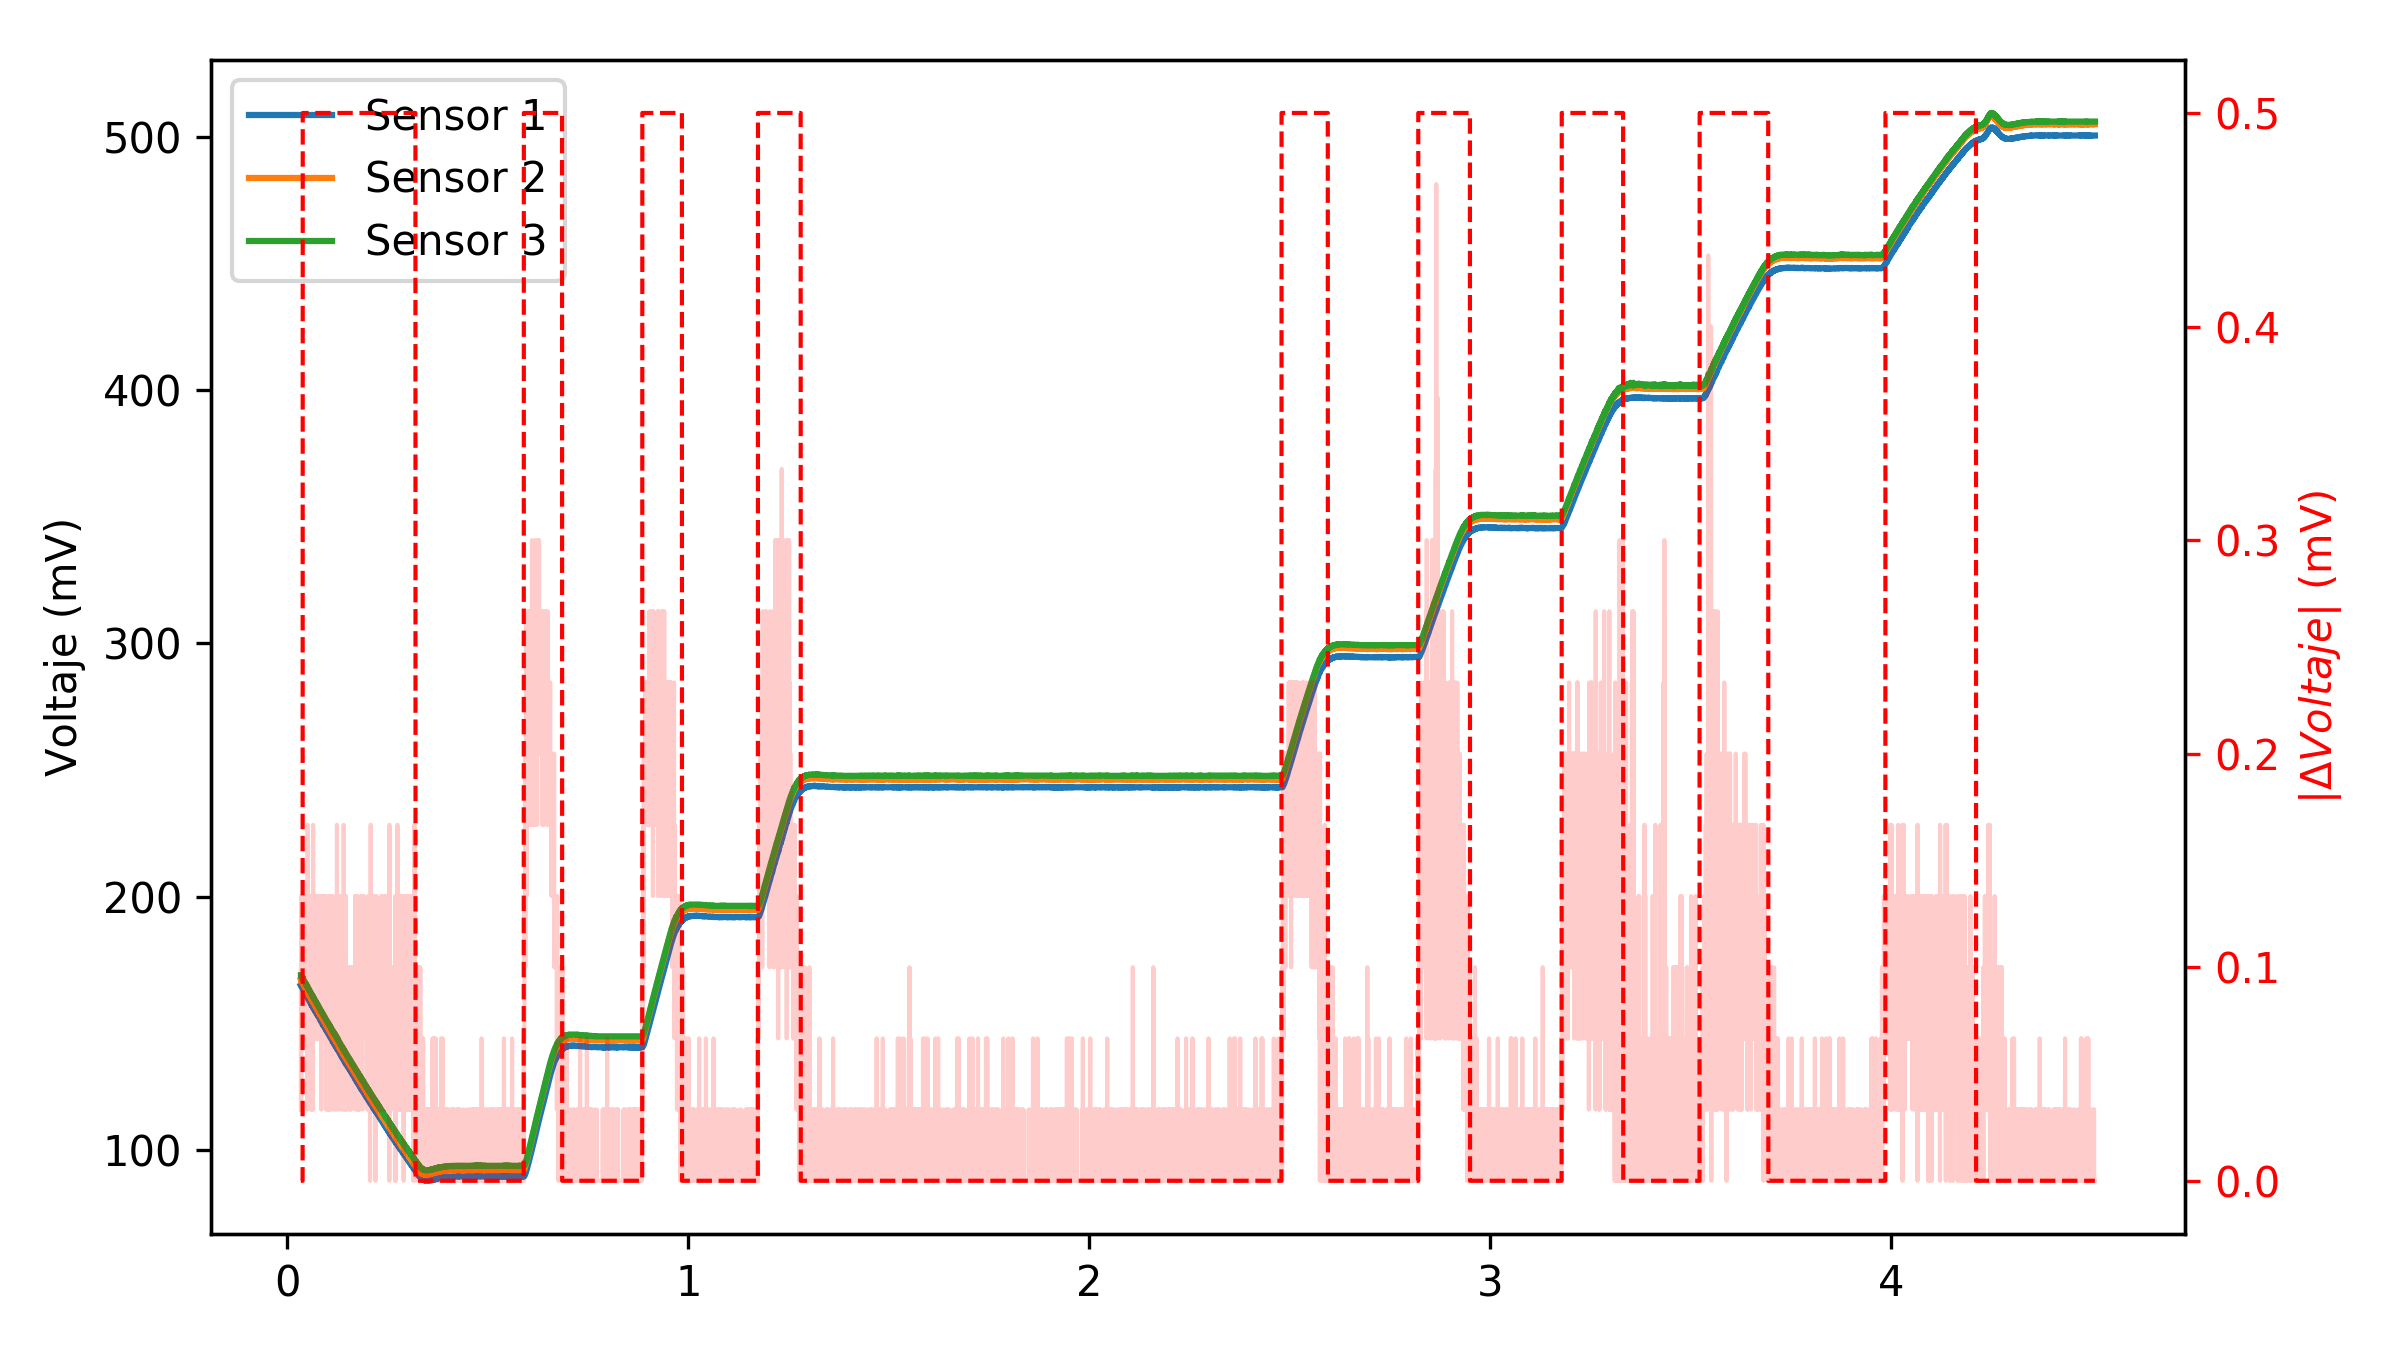
\includegraphics[width=\linewidth]{../Data/TemperatureCalibration/dV-t}
		\caption{Voltajes registrados en la rampa de calentamiento de calibración de los sensores.}
		\label{fig: calAlgorithm}
	\end{figure}

	Los valores de voltaje de los intervalos estacionarios de la rampa fueron relacionados con la temperatura del termómetro de mercurio en la \autoref{fig: voltageTemperature}, en donde se observó una tendencia lineal, cuya pendiente es cercana a 10 mV, lo cual concuerda con lo reportado por el fabricante \cite{instruments1999lm35}. A partir de las relaciones obtenidas con la regresión lineal, se reconstruyó la \autoref{fig: calAlgorithm} en función de la temperatura.
	\begin{figure}[h]
		\centering
		\begin{subfigure}{0.45\linewidth}
			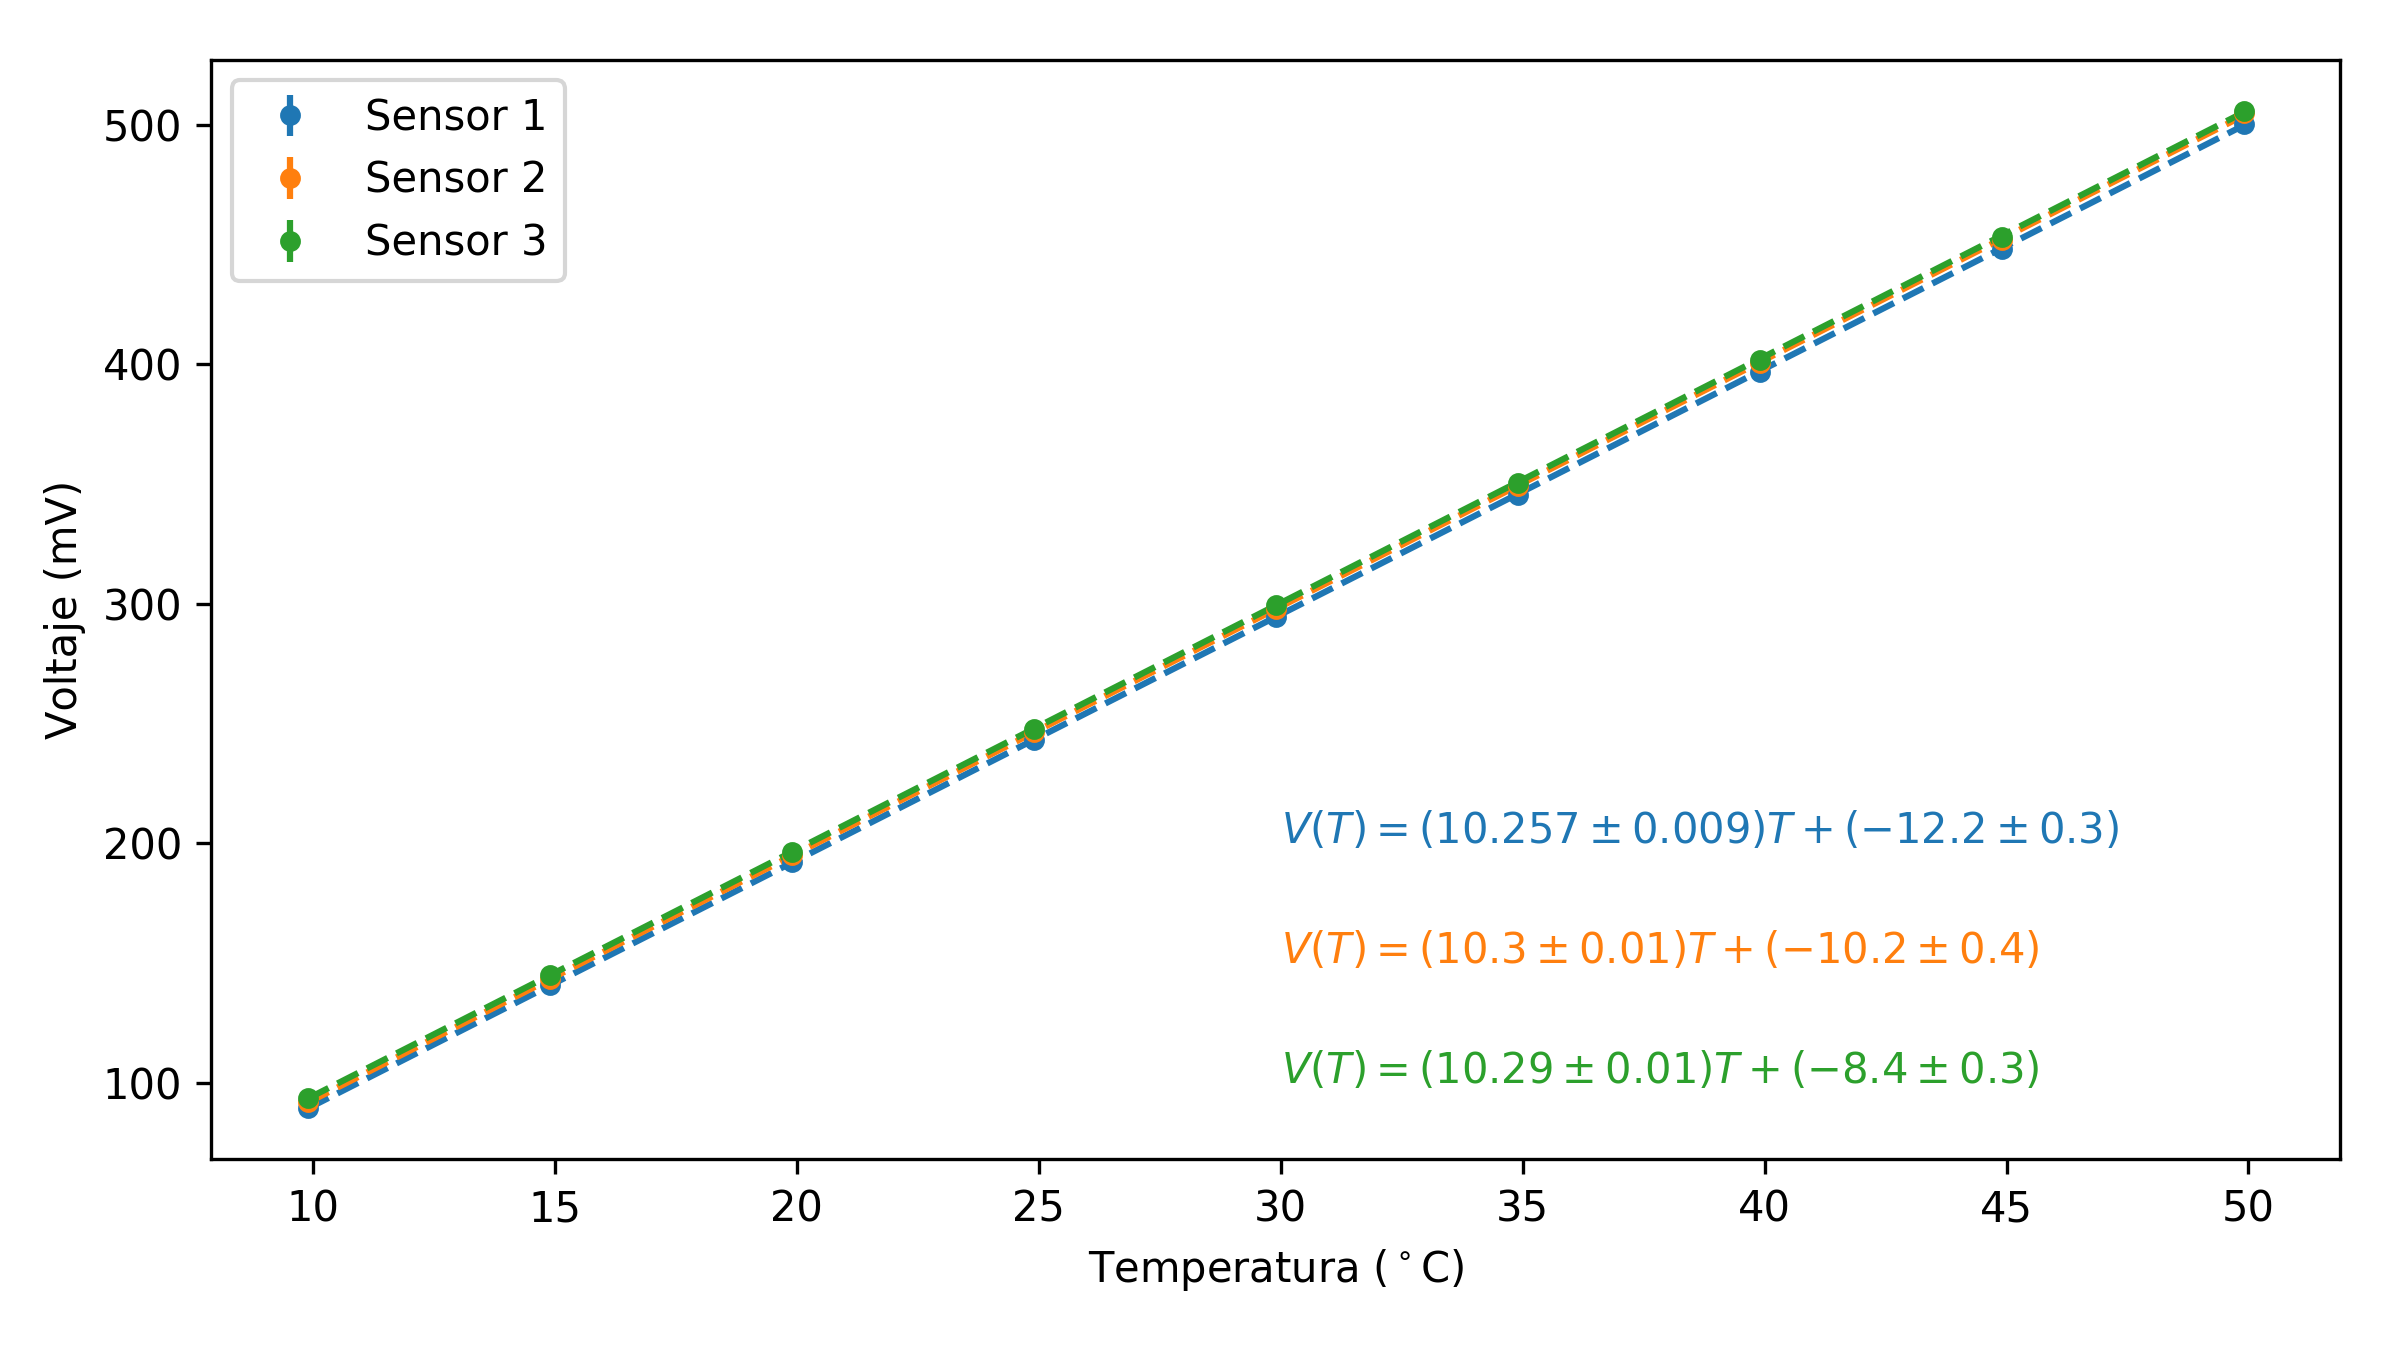
\includegraphics[width=\linewidth]{../Data/TemperatureCalibration/V-T}
			\caption{Voltajes registrados en la rampa de calentamiento de calibración de los sensores.}
		\end{subfigure}
		\begin{subfigure}{0.45\linewidth}
			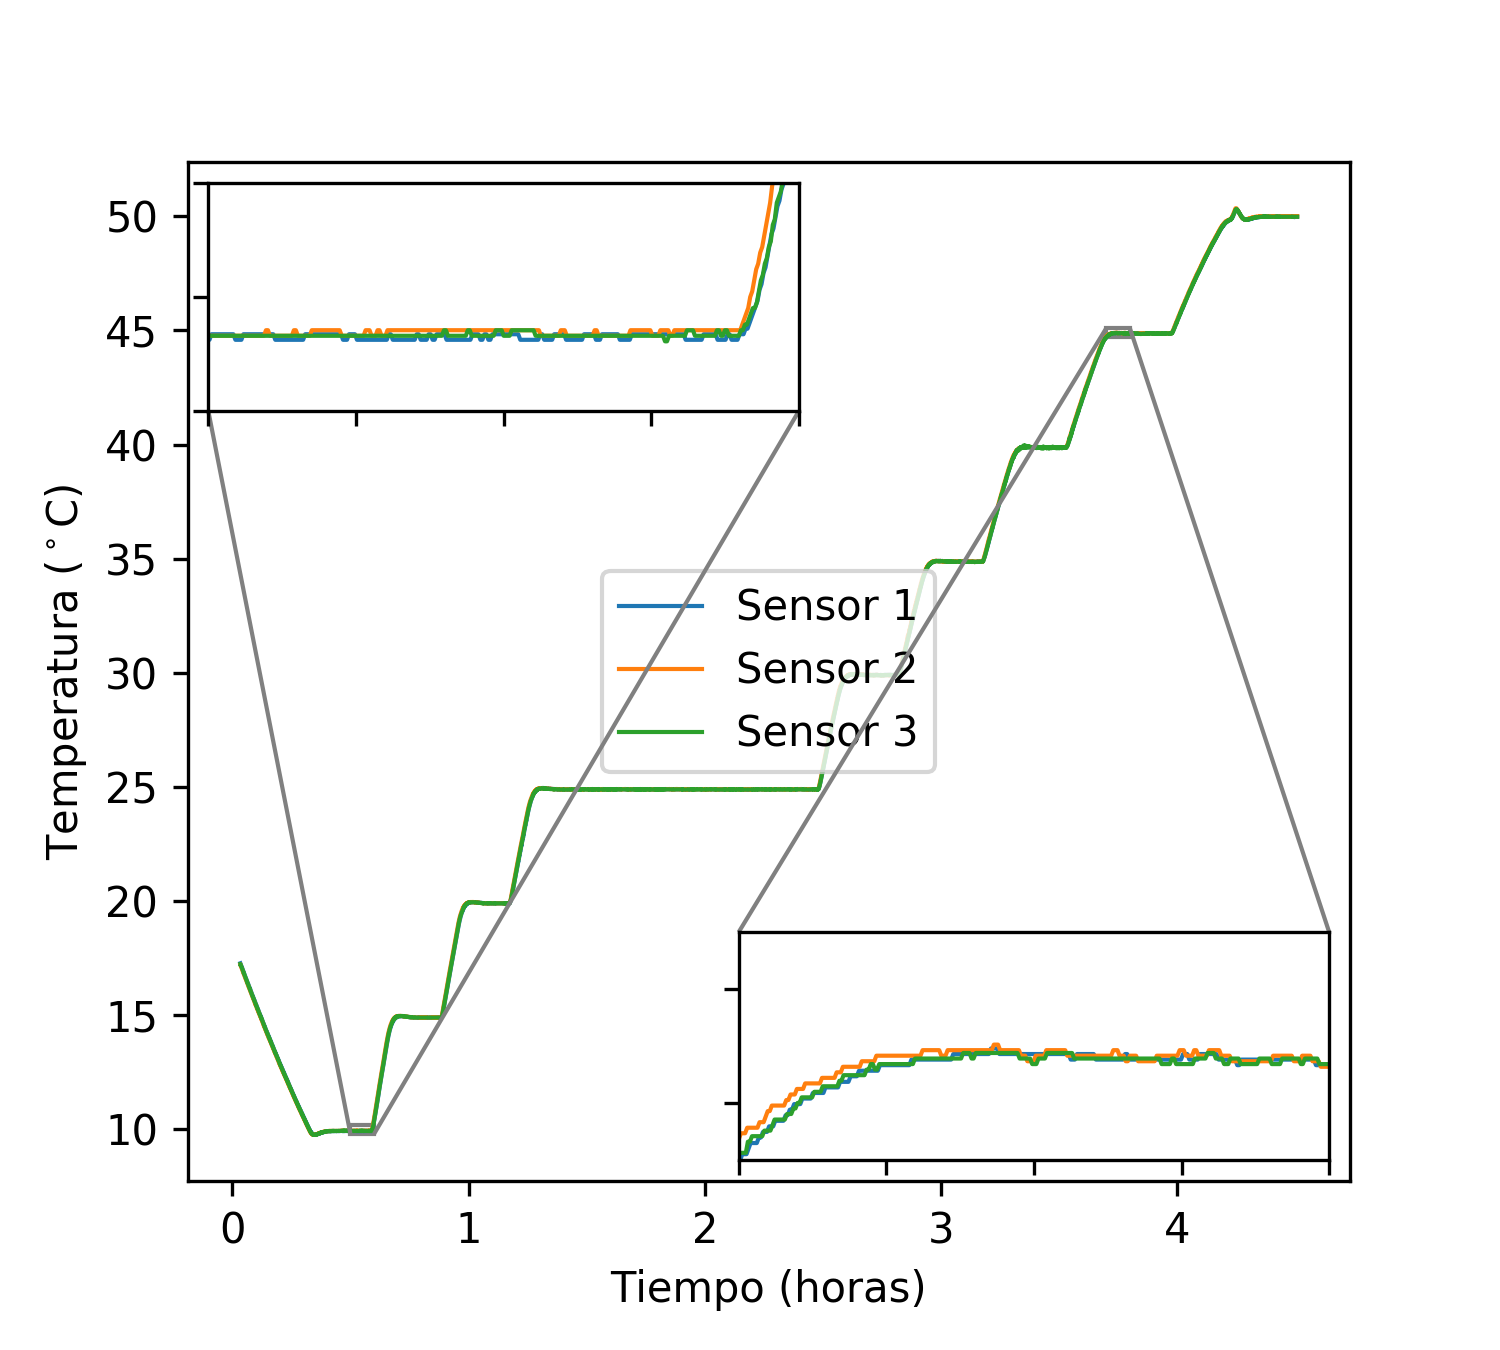
\includegraphics[width=\linewidth]{../Data/TemperatureCalibration/T-t}
			\caption{Voltajes registrados en la rampa de calentamiento de calibración de los sensores.}
		\end{subfigure}
		\caption{Resultados de la calibración del sistema de monitoreo de la temperatura.}
		\label{fig: voltageTemperature}
	\end{figure}
	\pagebreak

	Una vez calibrados los sensores, se escribió un programa en Python para facilitar la visualización de los datos en tiempo real, cuyo código se encuentra en la \autoref{anx: interfaz}. Además, para introducir el sensor usado en el baño interno del calorímetro sin que este estuviera expuesto directamente a la temperatura ambiente, se imprimió una tapa en 3D con un filamento de PLA (ácido poliláctico) para usar uno de los espacios reservados para un cilindro de medición del calorímetro.
	\begin{figure}[h]
		\centering
		\begin{subfigure}{0.45\linewidth}
			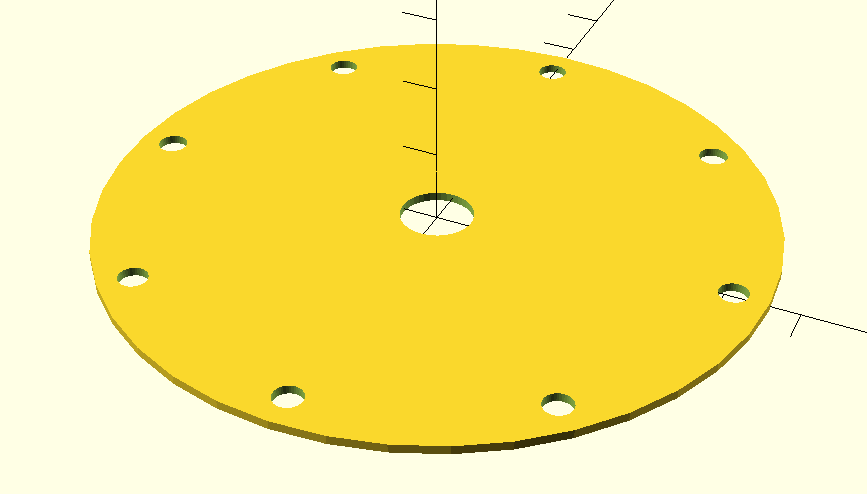
\includegraphics[width=\linewidth]{Figures/PLAdisk}
			\caption{Disco impreso para facilitar el acceso del sensor al baño térmico del calorímetro.}
		\end{subfigure}
		\begin{subfigure}{0.45\linewidth}
			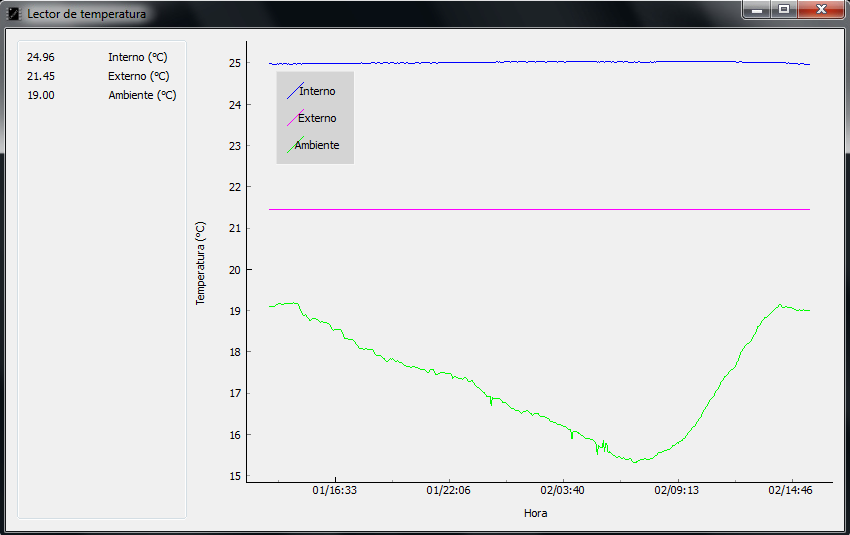
\includegraphics[width=\linewidth]{Figures/temperatureReader}
			\caption{Interfaz gráfica para el monitoreo de la temperatura en tiempo real.}
		\end{subfigure}
		\caption{Accesorios para el sistema de monitoreo de temperatura.}
	\end{figure}

	Con el monitoreo de temperatura establecido fue posible determinar el efecto del baño térmico externo sobre la temperatura del calorímetro. Por ejemplo, para el caso de las oscilaciones que se muestran en la \autoref{tb: temperatureRegister}, se encuentran relacionadas con la temperatura del baño externo, para el caso de temperaturas muy bajas del baño externo se observa que la temperatura del baño interno se encuentra estable, sin embargo los calefactores se encuentran trabajando fuera del rango completamente prendidos, y a temperaturas del baño externo intermedias, la temperatura del baño interno oscila. Esto se puede entender si se considera que los sistemas térmicos presentan inercia, por lo cual mientras el sensor de temperatura registra una temperatura menor a la deseada, aplicará sobre los calentadores potencia, una vez se sobre pase este valor los calentadores se apagarán pero el agua de los alrededores se continuará calentando por algún tiempo, posteriormente el sistema detectará que la temperatura ha disminuído prendiendo nuevamente los calentadores haciendo que la temperatura en general oscile como se muestra en la \autoref{fig: temperatureRipple}.
	\begin{figure}[h]
		\centering
		\begin{subfigure}{0.49\linewidth}
			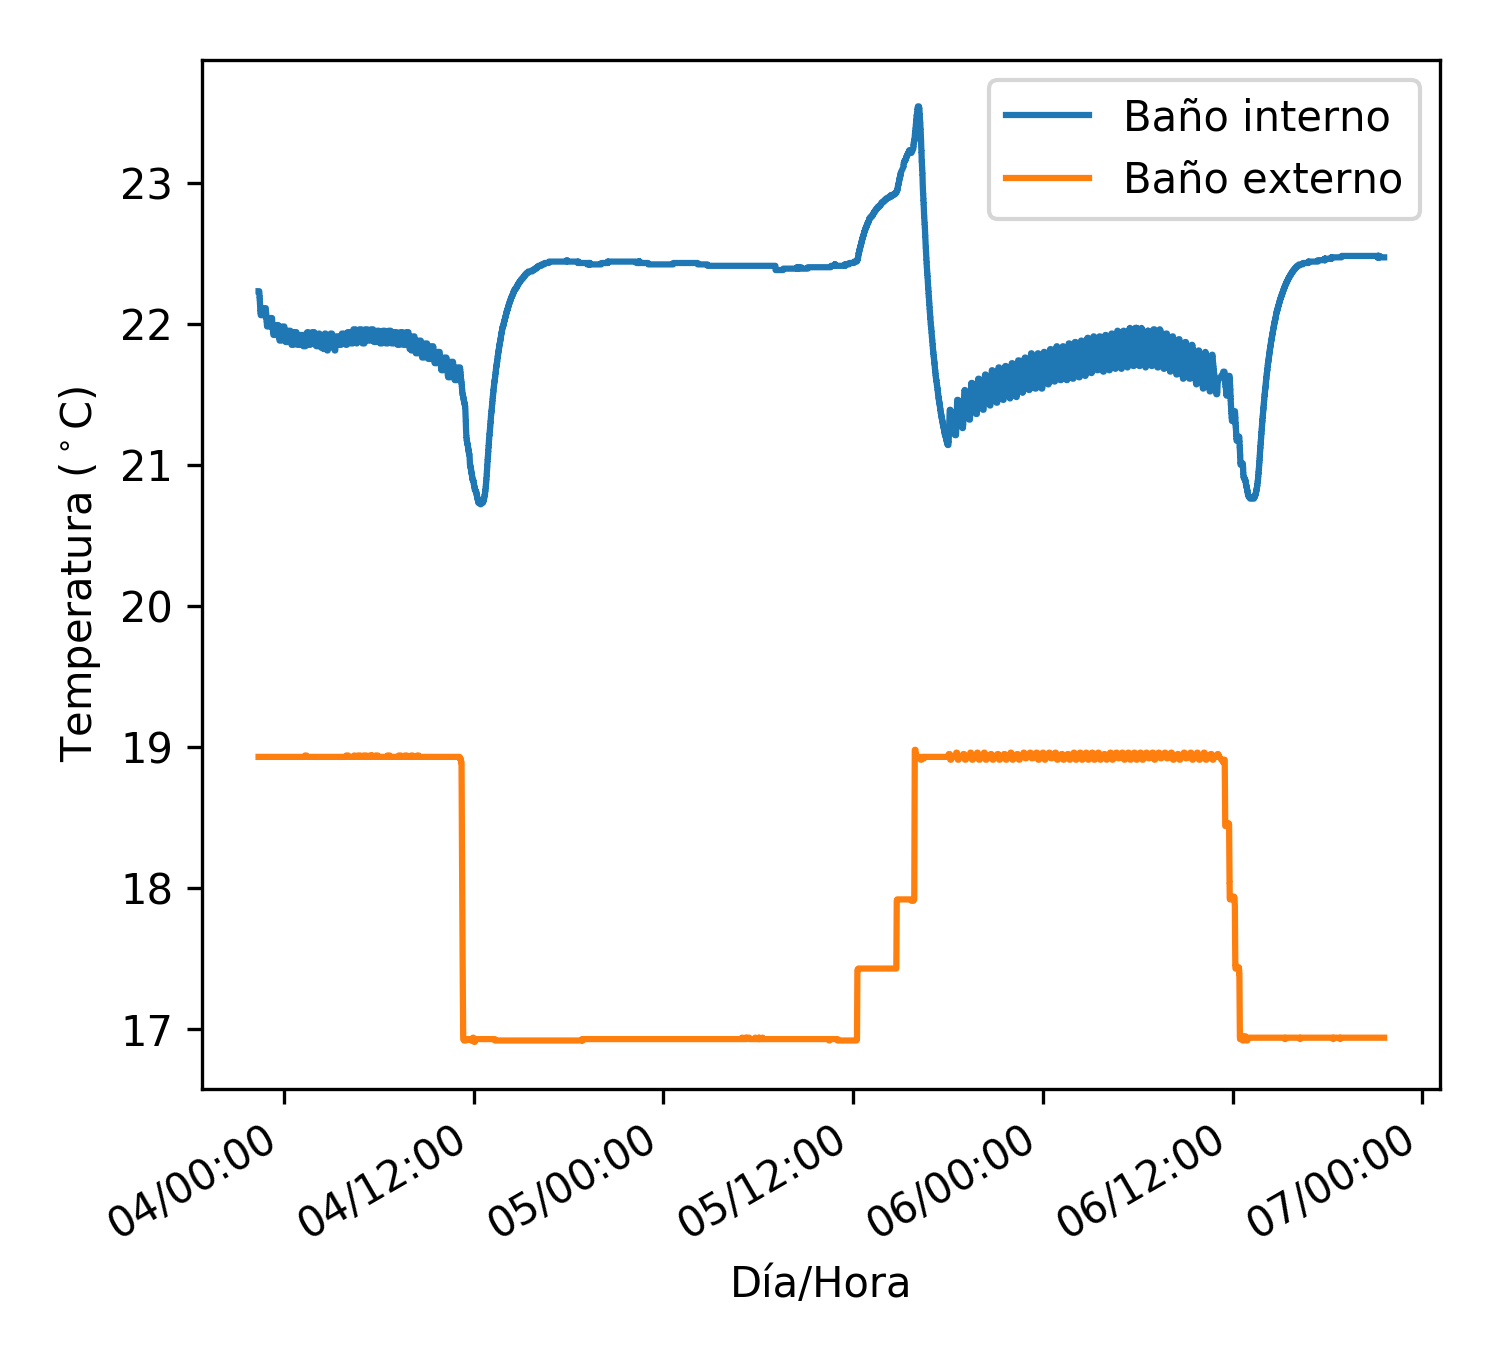
\includegraphics[width=\linewidth]{../Data/TemperatureStability/temperatureRipple}
			\caption{Oscilaciones debidas a una temperatura del baño externo intermedia.}
			\label{fig: temperatureRipple}
		\end{subfigure}
		\begin{subfigure}{0.49\linewidth}
			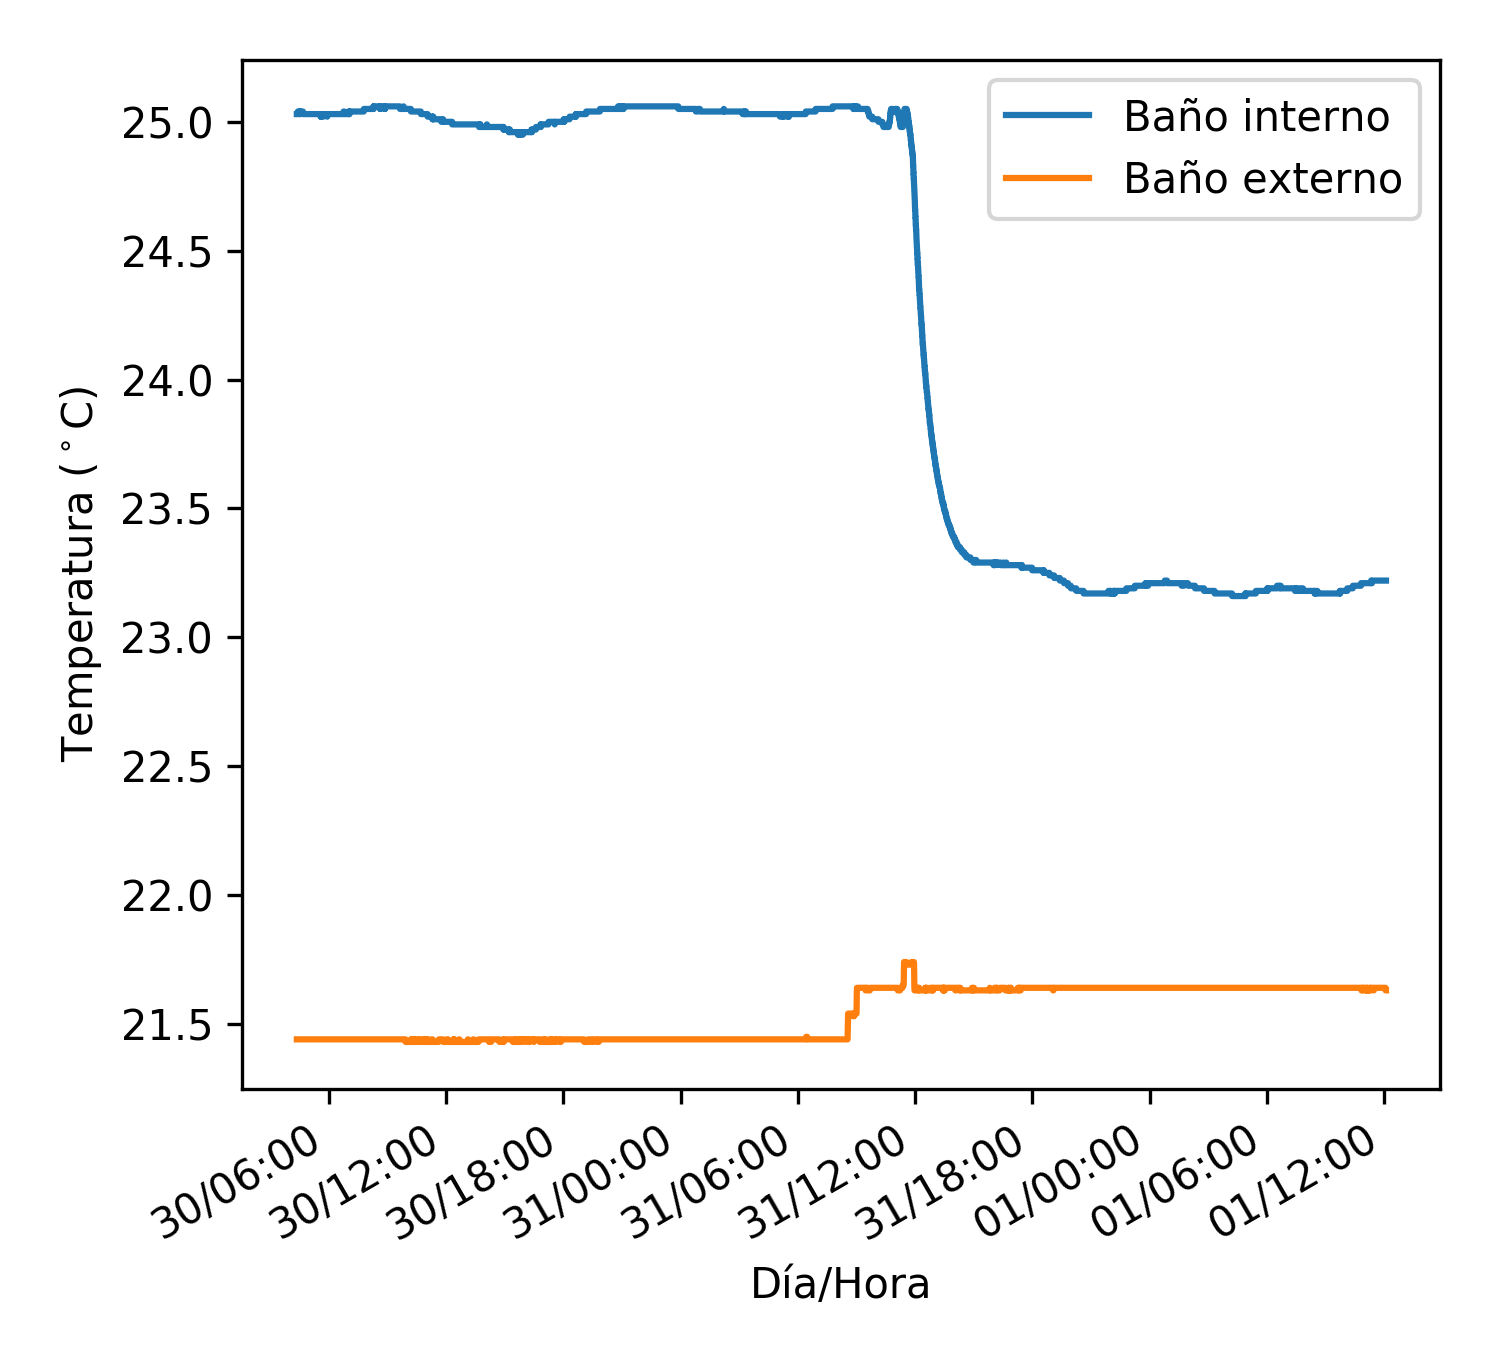
\includegraphics[width=\linewidth]{../Data/TemperatureStability/temperatureSensibility}
			\caption{Caída de la temperatura del baño interno debido al aumento de 0,20 \grad{} en el baño externo.}
			\label{fig: temperatureSensibility}
		\end{subfigure}
		\caption{Efecto de la temperatura del baño externo sobre la temperatura del baño interno.}
		\label{fig: externalEffects}
	\end{figure}

	En la \autoref{fig: temperatureSensibility} se observa cómo la temperatura del calorímetro puede variar bruscamente cuando los calentadores trabajan fuera de rango. En el caso de esta figura, la temperatura del calorímetro se encontraba estable, el calentador fino siempre en el rango de trabajo, mientras que el precalentador ocasionalmente salía del rango de trabajo, sin embargo, al aumentar la temperatura del baño 0,20 \grad{} el equipo disminuyó su temperatura y no volvió aumentar. 
	
	En general la \autoref{fig: externalEffects} muestra la dificultad de estabilizar el equipo a una temperatura determinada, puesto que se debe encontrar la pareja correcta de valores en las resistencias de décadas, junto con la temperatura del baño externo, siendo los dos particularmente sensibles al valor del otro. Pues como fue mencionado anteriormente, aunque en la \autoref{fig: temperatureSensibility} el sistema parezca estable, los calentadores internos están funcionando fuera del rango.
	
	Finalmente, se logró determinar la configuración en donde los calentadores se encuentran en el rango de trabajo y el equipo es estable a $25.02 \pm 0.03$ \grad{}, esta configuración se muestra en la \autoref{tb: decadeResistorsAfter}. Además, el sensor de temperatura ambiente, probó ser útil, pues la pequeña variación en la temperatura interna del calorímetro se encuentra correlacionada con la temperatura ambiente, pues en la \autoref{fig: temperatureResults} se observa que los máximos de temperatura interna ocurren en los mínimos de temperatura ambiente.
	\begin{table}[h]
		\centering
		\caption{Valores de las resistencias de década, para una temperatura de 25 \grad{}, obtenida en octubre.}
		\begin{tabular}{r|cccc|l}
			\hline
			\textbf{Baño interno (\grad{})} & A ($10^4$ $\Omega$) & B ($10^3$ $\Omega$) & C ($10^2$ $\Omega$) & D ($10^1$ $\Omega$) & \textbf{Baño externo (\grad{})} \\
			\hline
			$25.02 \pm 0.03$ & 3 & 3 & 6 & 5 & 21,5 \\
			\hline
		\end{tabular}
		\label{tb: decadeResistorsAfter}
	\end{table}

	\begin{figure}[h]
		\centering
		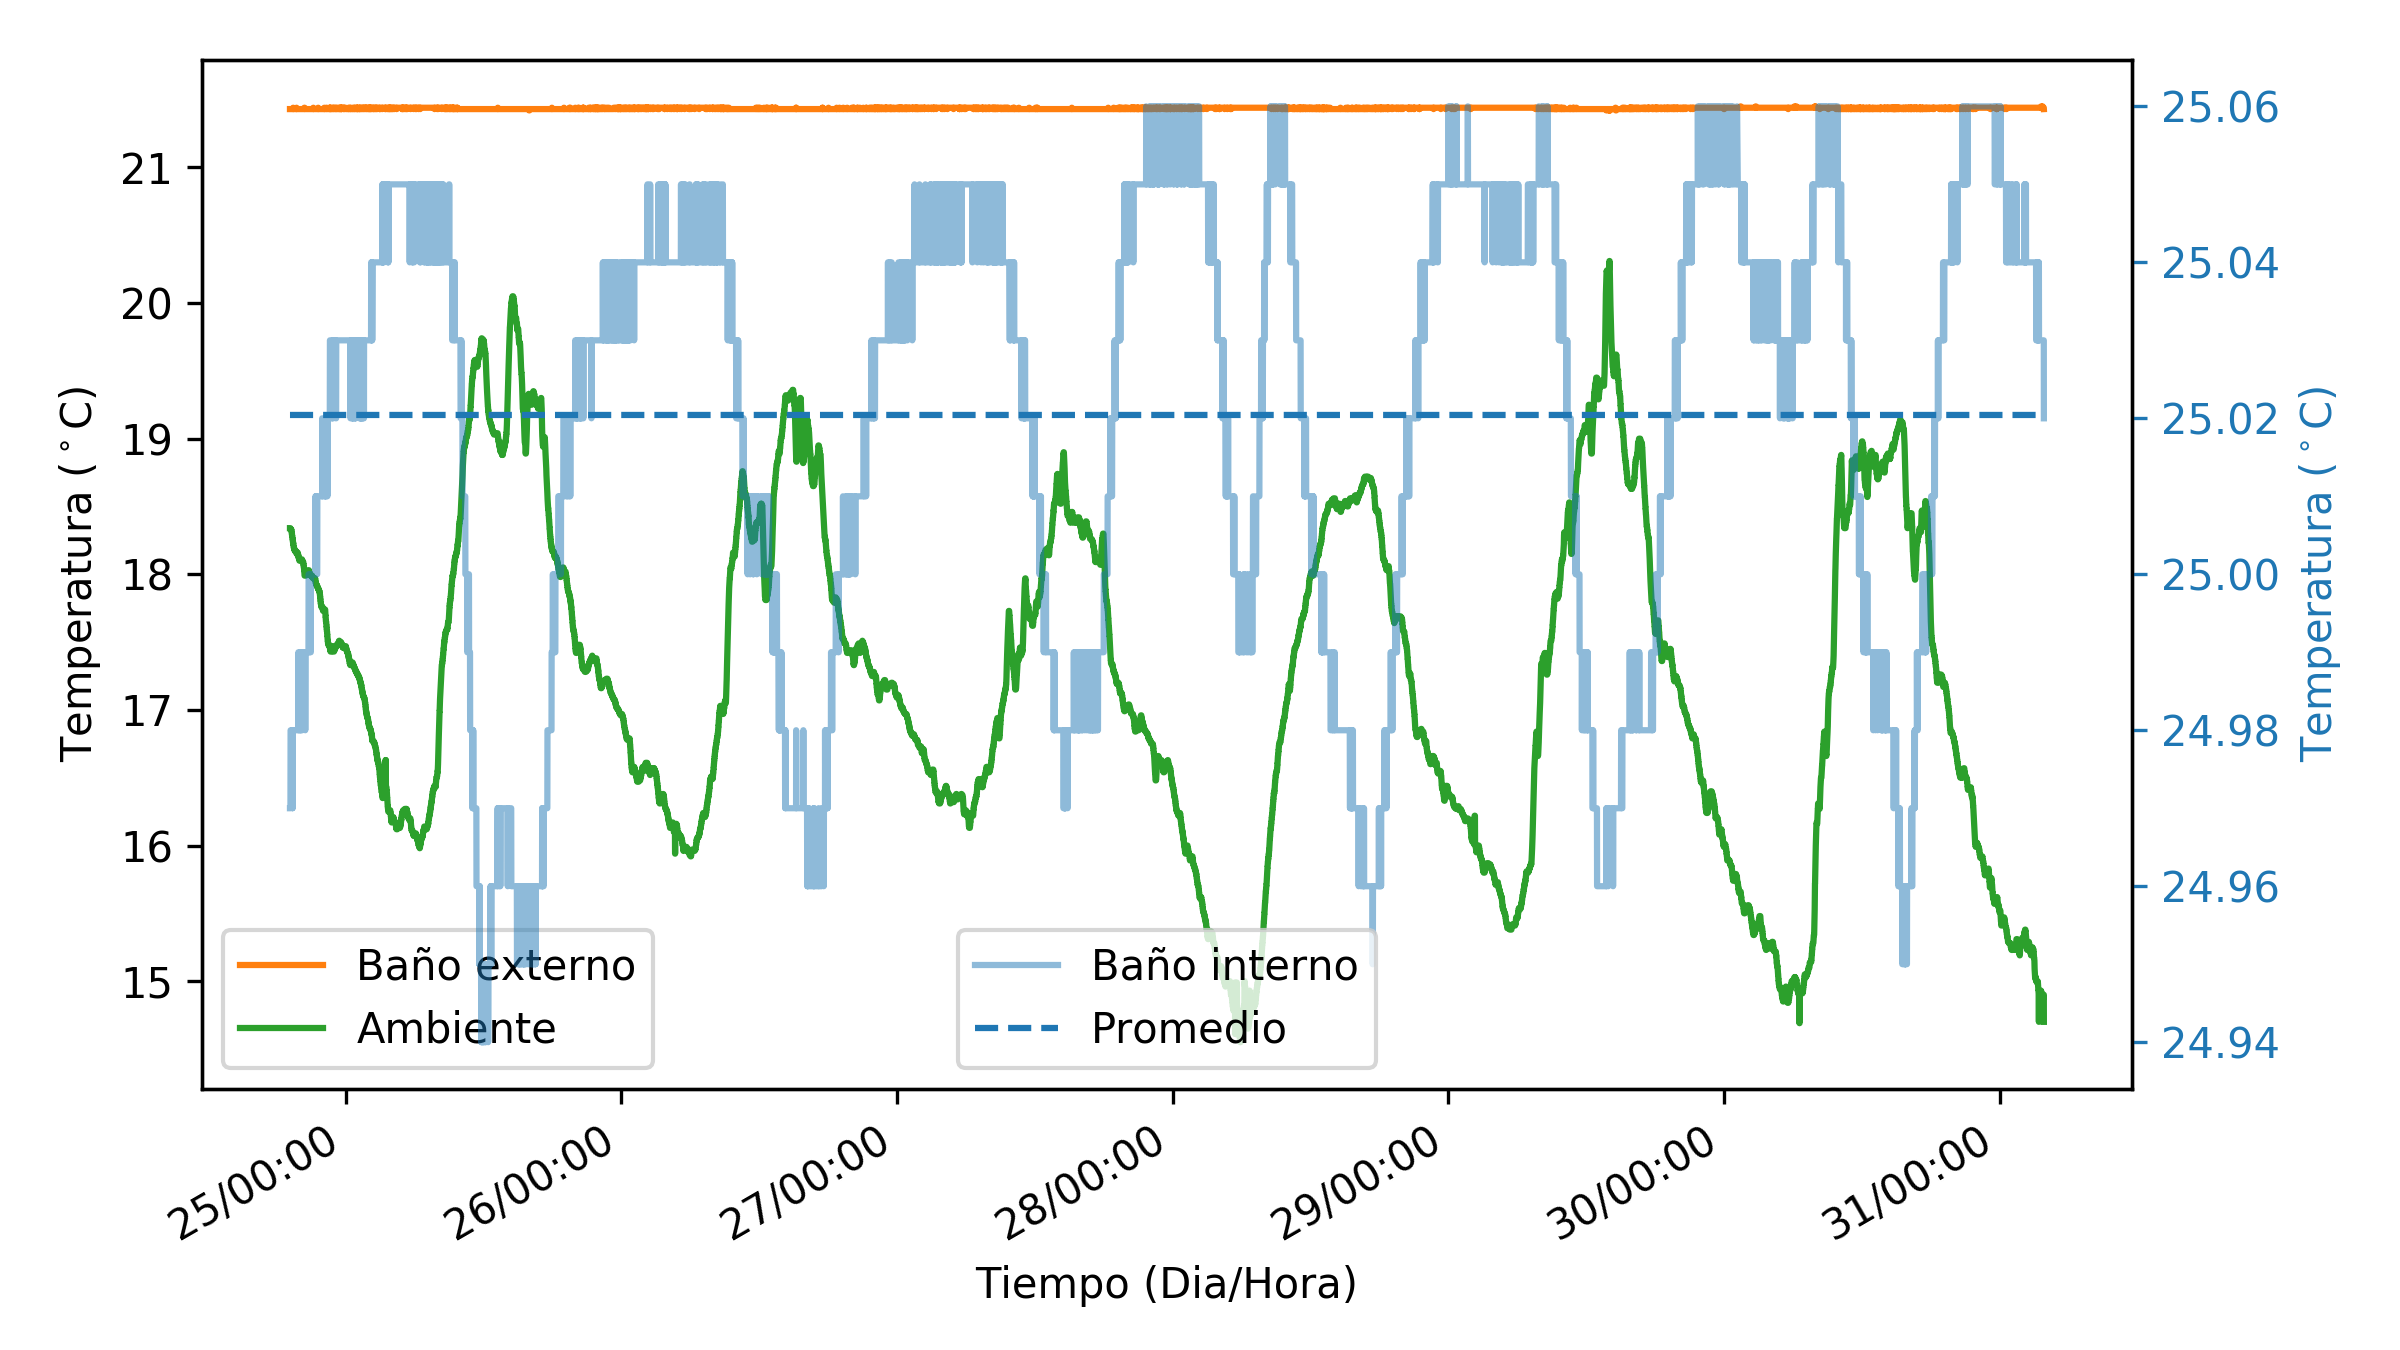
\includegraphics[width=\linewidth]{../Data/TemperatureStability/temperatureStability}
		\caption{Efecto de la temperatura del baño externo sobre la temperatura del baño interno.}
		\label{fig: temperatureResults}
	\end{figure}
% !TeX spellcheck = es_ES
% Chapter 1

%\chapter{Chapter Title Here} % Main chapter title
%
%\label{Chapter1} % For referencing the chapter elsewhere, use \ref{Chapter1} 

%----------------------------------------------------------------------------------------

% Define some commands to keep the formatting separated from the content 
%\newcommand{\keyword}[1]{\textit{#1}}
%\newcommand{\tabhead}[1]{\textbf{#1}}
%\newcommand{\code}[1]{\texttt{#1}}
%\newcommand{\file}[1]{\texttt{\bfseries#1}}
%\newcommand{\option}[1]{\texttt{\itshape#1}}

%----------------------------------------------------------------------------------------

\chapter{Calibración Eléctrica}
	Con el objetivo de asegurar que la información registrada por el calorímetro corresponde con un valor específico de potencia, es necesario realizar una calibración eléctrica, la cual es específica para cada canal de medición. Para ello, el equipo cuenta con una resistencia de precisión que envuelve el contenedor de la celda y permite simular, lo mejor posible, la energía liberada en forma de calor cuando una reacción química tiene lugar en la celda, la ubicación de esta resistencia se muestra en la \autoref{fig: resistencia} \cite{Suurkuusk}. 
	\begin{figure}[h]
		\centering
		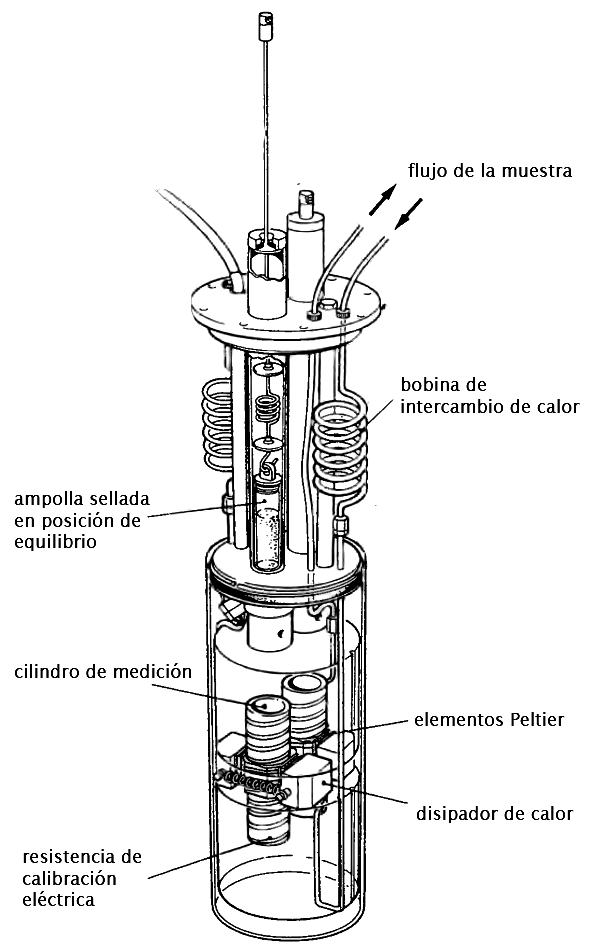
\includegraphics[width=0.45\linewidth]{Figures/resistencia}
		\caption{Interior del cilindro de medición, modificidado de \cite{Suurkuusk}.}
		\label{fig: resistencia}
	\end{figure}
	
	Para calibrar el sistema se realizan lecturas consecutivas de la línea base, esto es la potencia que registra el calorímetro es ausencia de perturbación, y a partir de esto se ajusta el cero del canal, pues se busca que la línea base sea lo más cercana a 0 $\mu$W. Posteriormente, se aplica una potencia conocida sobre la resistencia y hacen lecturas de la potencia registrada por el calorímetro, a partir de esto se ajusta la ganancia, hasta que la potencia aplicada y la registrada tengan el valor más cercano posible. La potencia conocida debe concordar con el valor de amplificación del selector \texttt{RANGE} en la \autoref{fig: controlCal}.
	\begin{figure}[h]
		\centering
		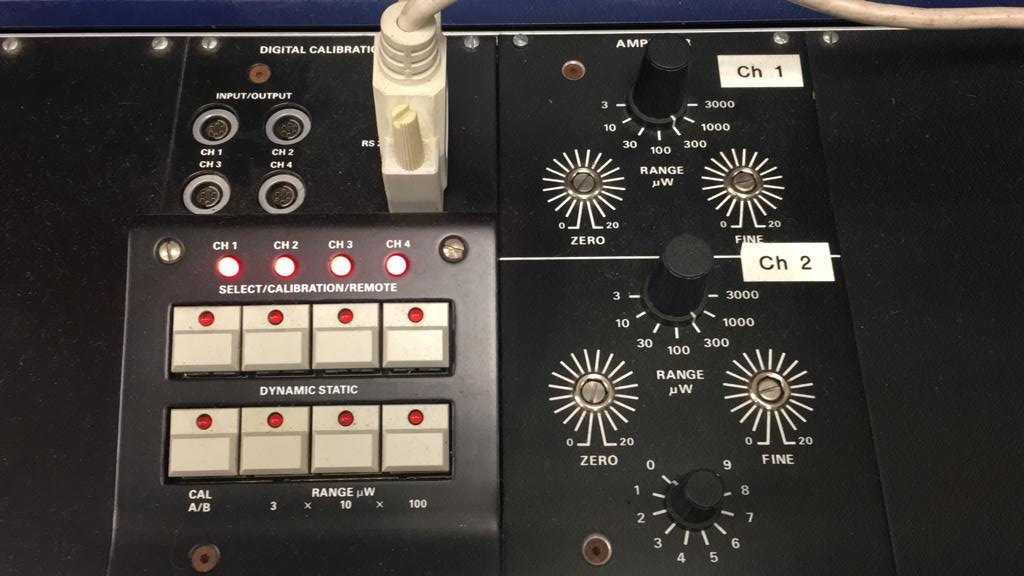
\includegraphics[width=0.7\linewidth]{Figures/controlCal}
		\caption{Control del cero y la ganancia del calor\'imetro}
		\label{fig: controlCal}
	\end{figure}
	
	Existen dos tipos de calibraciones, en la primera se modifican los valores de cero y ganancia en el equipo directamente, mientras que en la segunda los valores corresponden a ajustes en el software. Estos métodos de calibración reciben el nombre de estática y dinámica correspondientemente, y se debe asegurar que al momento de realizar una calibración dinámica, una calibración estática haya sido realizada previamente, pues los valores registrados por software son digitales (discretos), entonces la resolución de estos será determinada por la ganancia del circuito análogo, lo cual sólo es posible de controlar en el calorímetro directamente.
	 
	\section{Est\'atica}
	En la calibración estática, se debe manipular el equipo directamente. En primer lugar como fue mencionado anteriormente se ajusta el cero del canal en ausencia de perturbaciones. Para esto se manipula el potenciómetro de diez vueltas del lado izquierdo el cual está marcado como \texttt{ZERO} en la \autoref{fig: controlCal}, girando en sentido horario el valor de potencia registrado será cada vez menor. Una vez el cero ha sido ajustado, se aplica sobre la resistencia una potencia conocida, por un tiempo determinado por el usuario, y se espera que la señal registrada por el calorímetro en su estado estacionario coincida con el valor aplicado de potencia. Para esto se debe esperar cerca de 20 minutos para que la resistencia alcance el estado estacionario y posteriormente se manipula el potenciómetro derecho (\texttt{FINE} en la \autoref{fig: controlCal}), donde giros en el sentido horario disminuyen el valor de potencia registrado por el equipo, de esta forma se configura la ganancia del equipo.

	Para activar la resistencia es posible hacerlo manualmente a través de los botones blancos que se observan en la \autoref{fig: controlCal}. En primer lugar se selecciona el canal sobre el cual se quiere realizar la calibración, para esto se oprime el botón correspondiente a cada canal (canal 1, botón izquierdo) del panel \texttt{SELECT}, esto ocasionará que la luz asociada a ese canal comience a oscilar. Posteriormente, si la luz continúa en este estado se debe volver a presionar el botón de \texttt{SELECT} asociado a este canal. El lado de la calibración A ó B se selecciona oprimiendo el botón \texttt{CAL A/B} donde la luz prendida indica A, y la potencia oprimiendo los botones de \texttt{RANGE} cuyo producto da el valor de potencia deseado en $\mu$W. Finalmente, para activar la calibración se oprimen de manera simultánea el botón de \texttt{SELECT} del canal y el botón \texttt{CAL A/B}. Una vez se haya calibrado el estado estacionario, la resistencia se apaga oprimiendo el botón del canal en \texttt{SELECT} y posteriormente, al mismo tiempo este botón y \texttt{CAL A/B}.
	
	Otra manera de hacerlo es a través del software Digitam. En donde se realiza un método experimental que contenga la calibración eléctrica, este método ya se encuentra creado bajo el nombre \texttt{staticCalibration.tam}, el cual:
	\begin{itemize}
		\item Mide por 30 minutos la línea base.
		\item Aplica 300 $\mu$W sobre el lado B del canal 1 (referencia) por 35 minutos.
		\item Espera por 45 minutos a que la potencia se estabilice en la línea base.
	\end{itemize}

	Resultados de calibraciones estáticas se muestran en la \autoref{fig: staticCalibrations}. En particular, para el caso de la \autoref{fig: noAmpCal} se tiene que el cero está bien ajustado, sin embargo el valor de la amplitud no corresponde, pues el sensor se satura a un valor de 213,9 $\mu$W, sin una transición suave al estado estacionario. El efecto contrario se observa en la \autoref{fig: noZeroCal}, pues la potencia aplicada corresponde con la leída, sin embargo, la línea base se encuentra a -80,1 $\mu$W.
	\begin{figure}[h]
		\centering
		\begin{subfigure}{0.45\linewidth}
			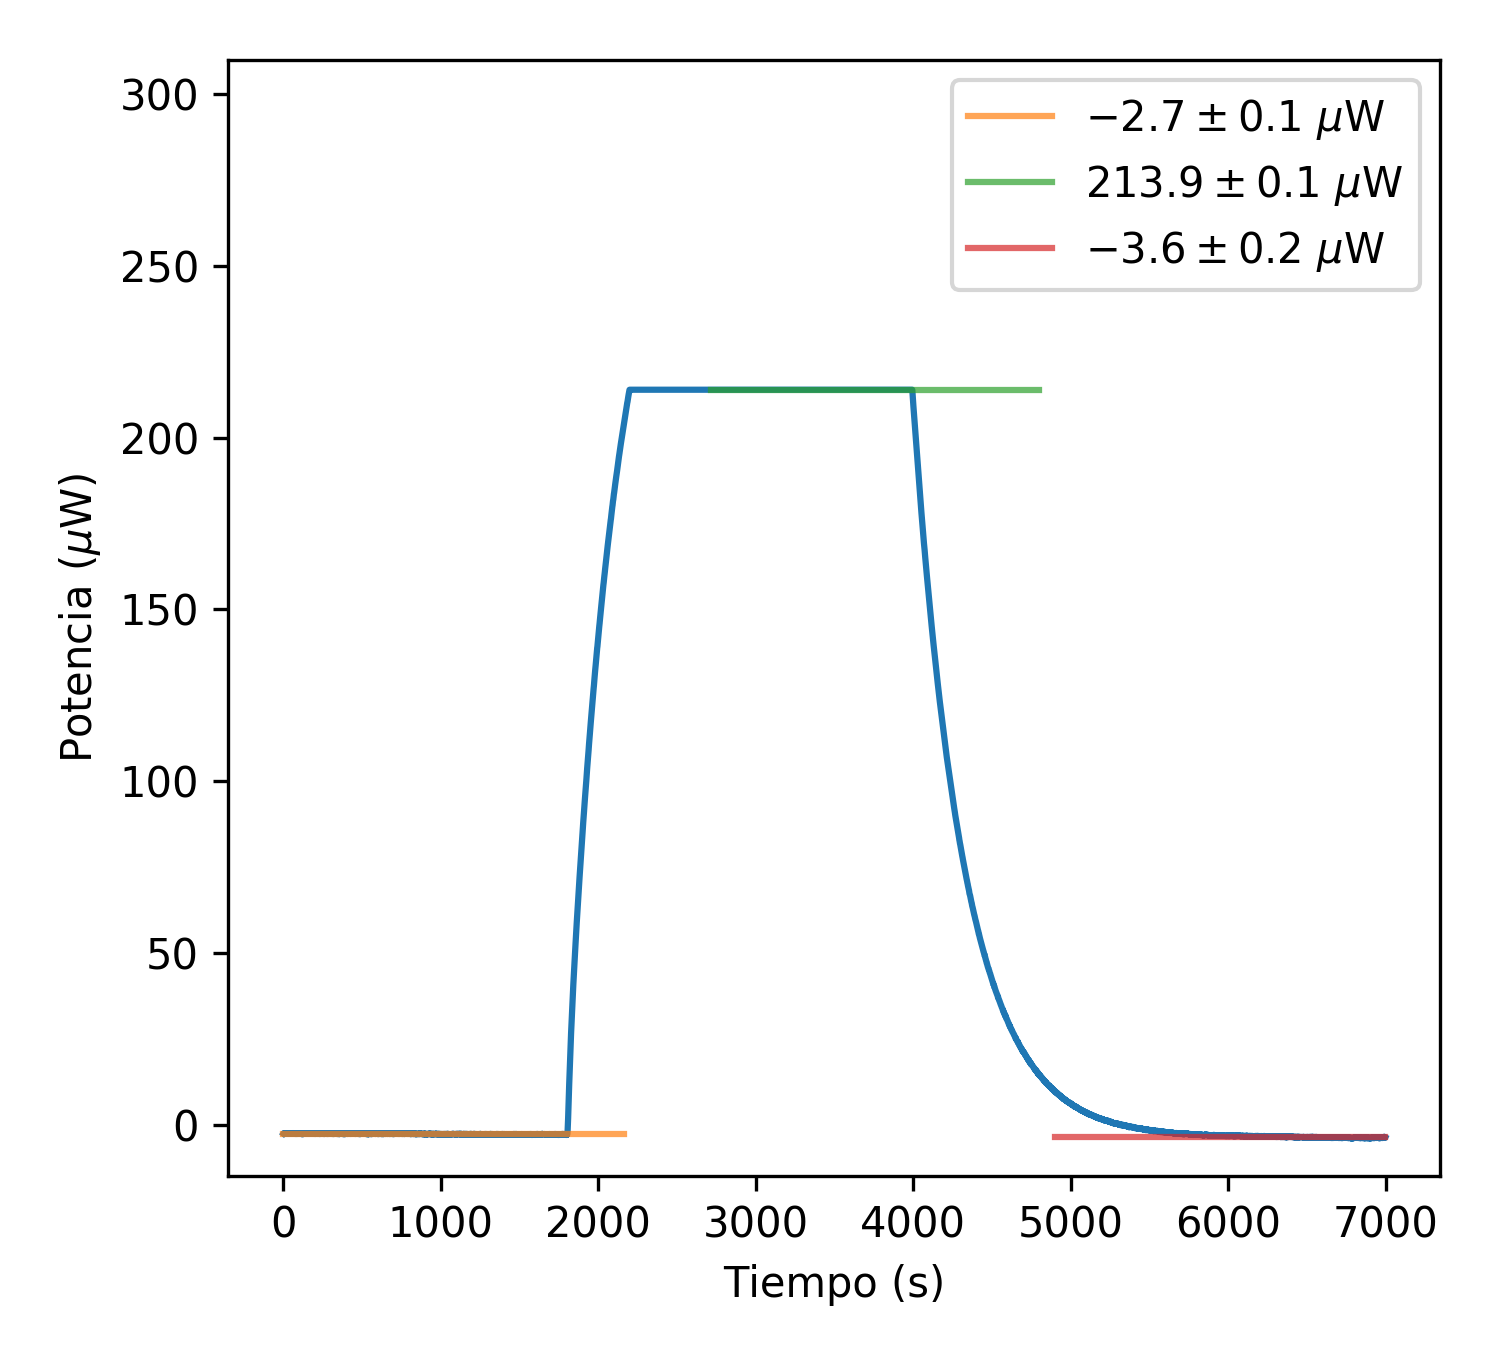
\includegraphics[width=\linewidth]{../Data/ElectricalCalibrations/Static/Calibration1}
			\caption{Potencia medida: $216.6 \pm 0.2$ $\mu$W.}
			\label{fig: noAmpCal}
		\end{subfigure}
		\begin{subfigure}{0.45\linewidth}
			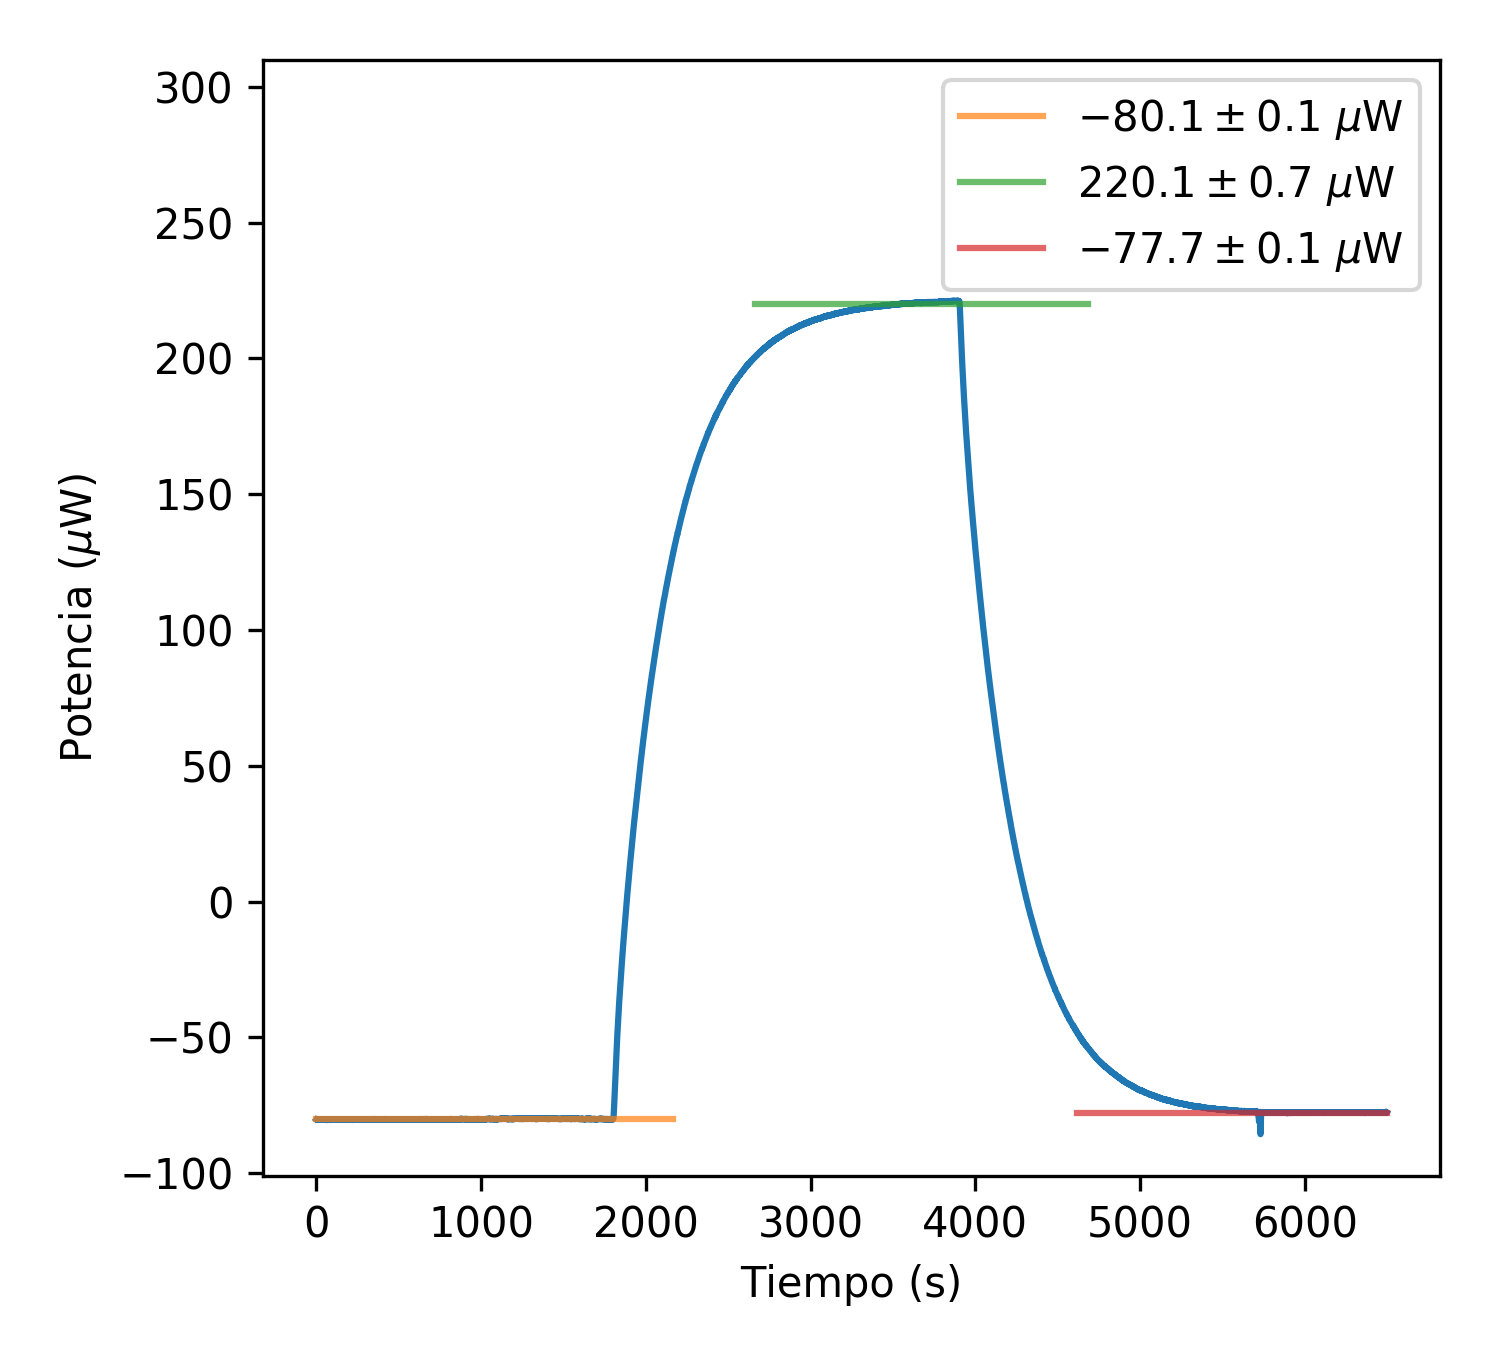
\includegraphics[width=\linewidth]{../Data/ElectricalCalibrations/Static/Calibration0}
			\caption{Potencia medida: $300.2 \pm 0.2$ $\mu$W.}
			\label{fig: noZeroCal}
		\end{subfigure}
		\caption{Ejemplos de calibraciones estáticas.}
		\label{fig: staticCalibrations}
	\end{figure}

	\newpage
	Para determinar las desviaciones a la línea base así como el valor del estado estacionario se implementó un algoritmo que se muestra en la \autoref{anx: staticCalibration} y que realiza lo siguiente:
	\begin{enumerate}
		\item Toma el valor absoluto de la derivada de la potencia.
		\item Realiza un filtro de medianas sobre los resultados anteriores, con un kernel de 101 puntos.
		\item A los puntos con valores mayores o iguales a 0,5 se les asigna un valor de 1, y los restantes 0.
		\item Se toma la derivada de los valores anteriores, de tal forma que aumentos corresponden con 1, y caídas con -1. Para el caso del estado estacionario y la última línea base, se toman el último 30 \% de los datos, en donde ya se encuentran estables estos estados. Las fronteras de estos valores determinan las fronteras de las líneas base y el estado estacionario.
		\item El promedio y desviación estándar se toma sobre cada uno de estos intervalos.
	\end{enumerate}
	
	\newpage
	\section{Din\'amica}
	En la calibración dinámica el sistema registra la línea base por 1 minuto, posteriormente aplica 40 \% de la potencia seleccionada sobre la resistencia, dando lugar a una pendiente constante por tres minutos, posteriormente, incremente nuevamente la potencia, mientras registra las pendientes observadas. Finalmente, la potencia se lleva hasta el 95 \% y se obtiene un corto estado estacionario, de esta forma el software ajusta los valores de ganancia y cero del canal \cite{Suurkuusk}. 
	\begin{figure}[h]
		\centering
		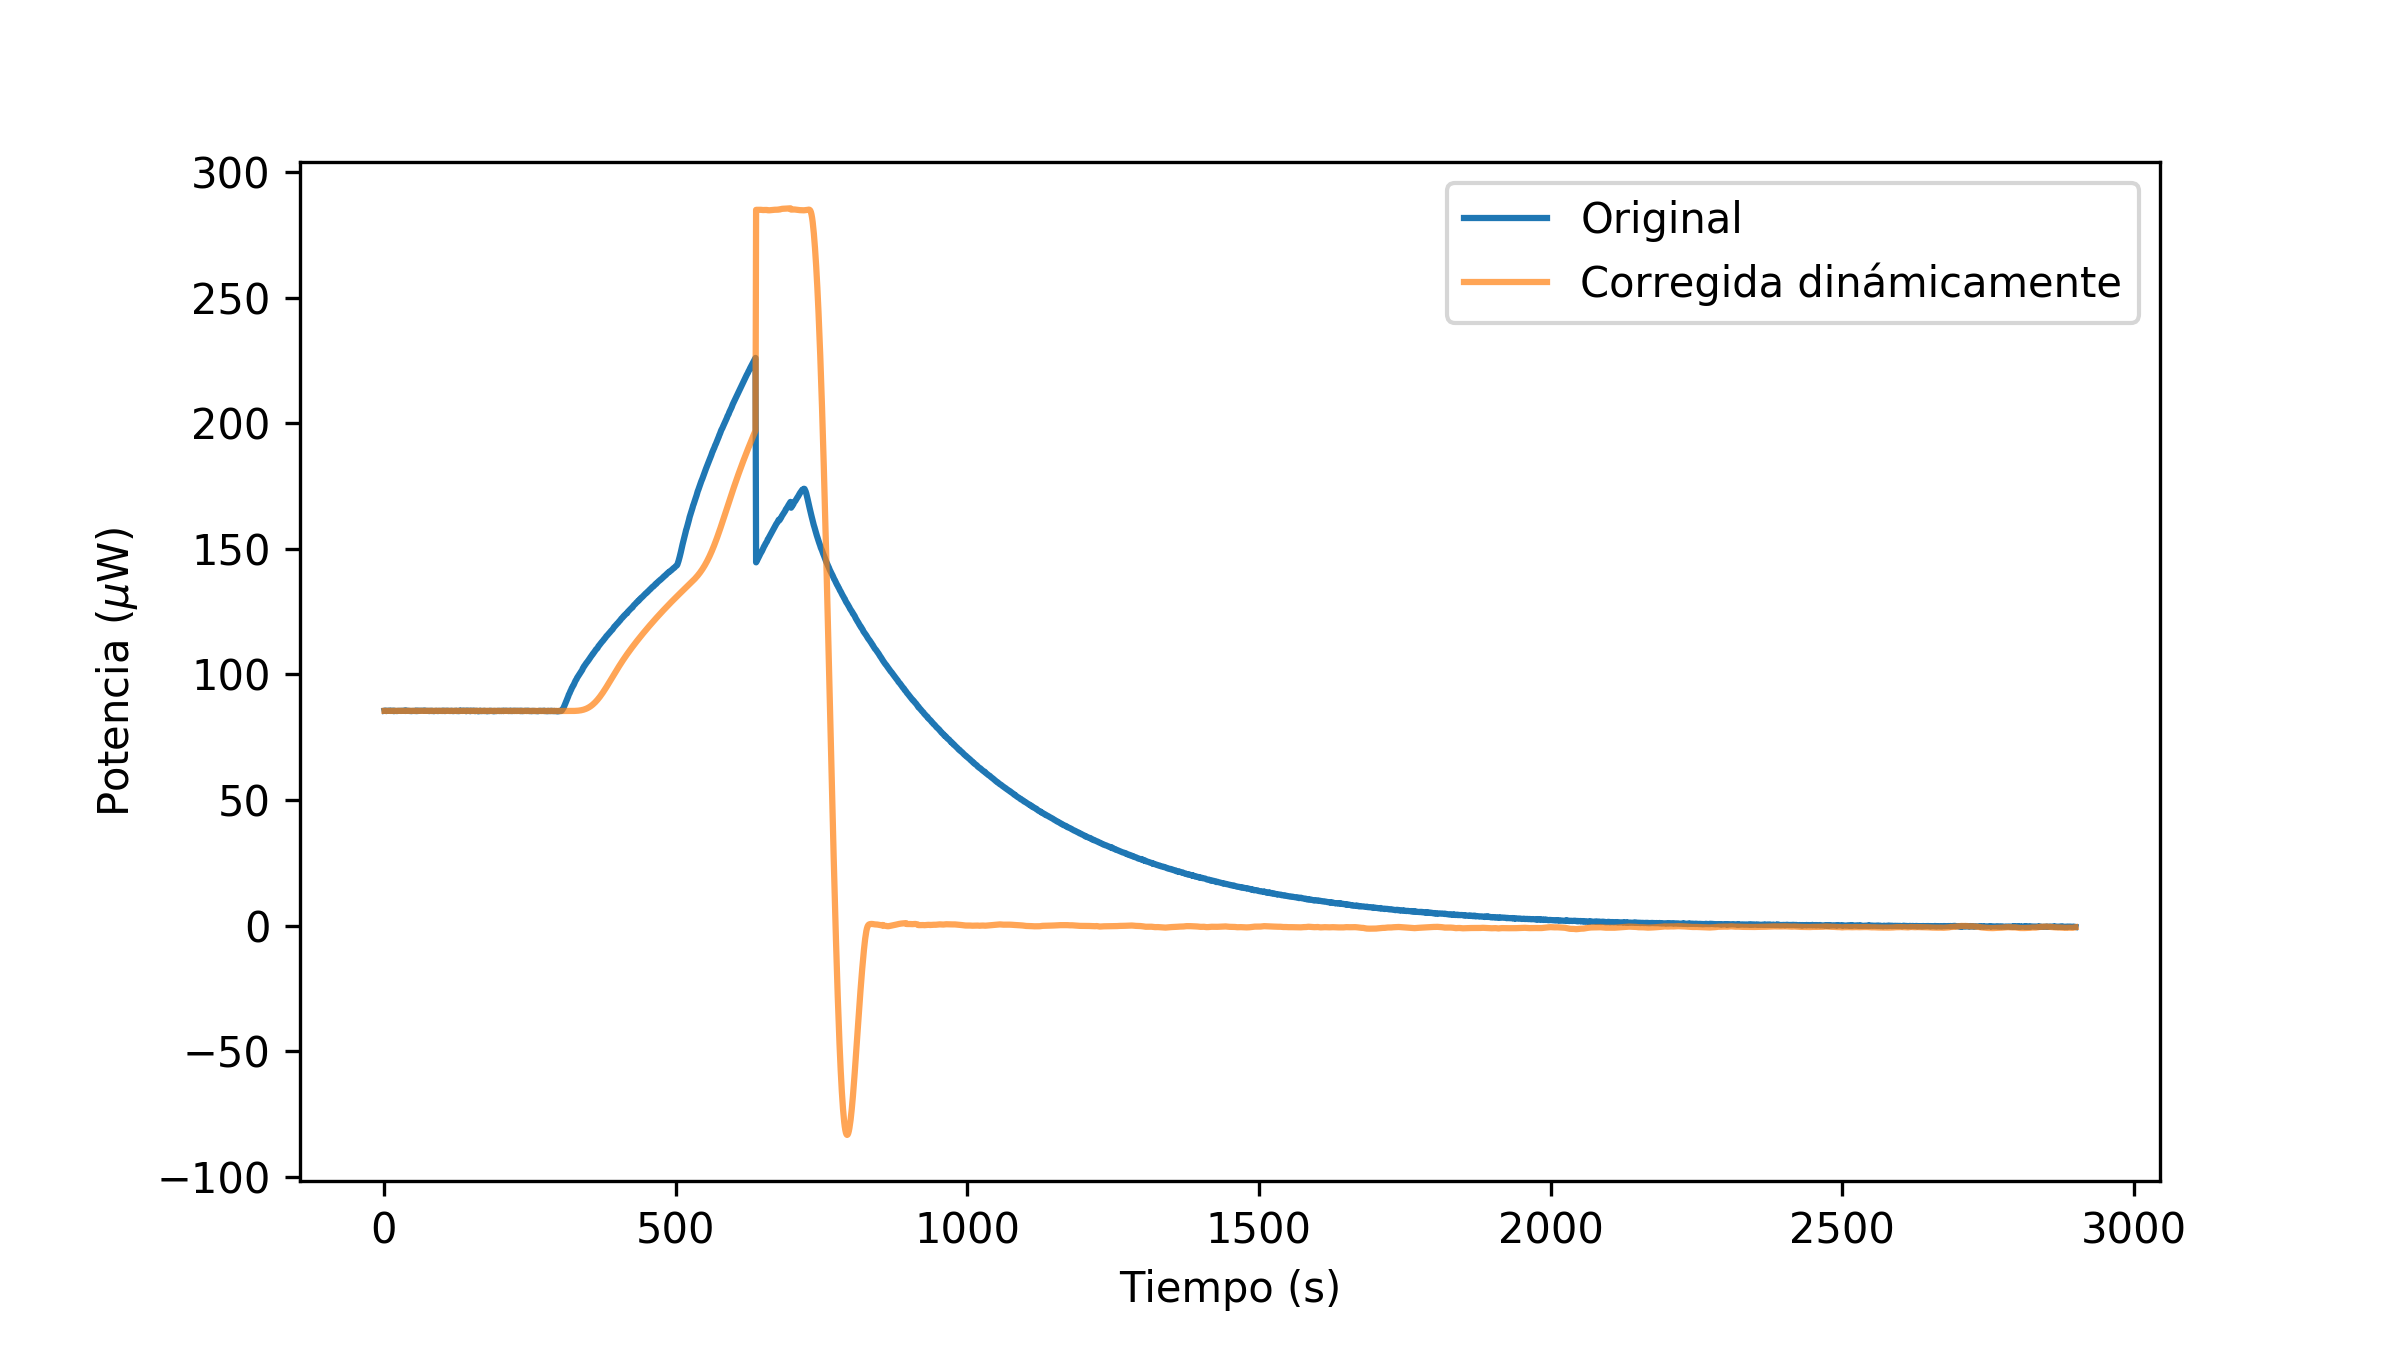
\includegraphics[width=\linewidth]{../Data/ElectricalCalibrations/Dynamic/dynamic}
		\caption{Ejemplo de una calibración dinámica.}
		\label{fig: dynamicCalibration}
	\end{figure}

	En la \autoref{fig: dynamicCalibration} se muestra un ejemplo de una calibración dinámica. En ella, la línea base se encuentra en 85,5 $\mu$W, luego de la calibración la línea base se estabiliza en -0,4 $\mu$W. La calibración dinámica permite caracterizar dos constantes que describen la inercia que presenta el calorímetro. Esto es que existe un tiempo de respuesta del equipo ante una perturbación. Luego de la calibración dinámica es posible tener una señal corregida dinámicamente, en donde se puede observar el estado estacionario al 95 \% de la potencia aplicada, y los cambios de pendiente que fueron antes mencionados.
	
	Finalmente, la calibración dinámica asegura la reproducibilidad de un experimento, como se muestra en la \autoref{fig: dynamicStatic}, en donde luego de haber realizado una calibración estática, se hace una dinámica y posteriormente para confirmar sus resultados se ejecuta una nueva calibración estática, en donde no se modifican ninguno de los parámetros en el calorímetro. En ella se observa como el inicio de las curvas de la calibración dinámica no coinciden, sin embargo, la parte final de estas se solapa, haciendo que las medidas sean reproducibles.
	\begin{figure}[h]
		\centering
		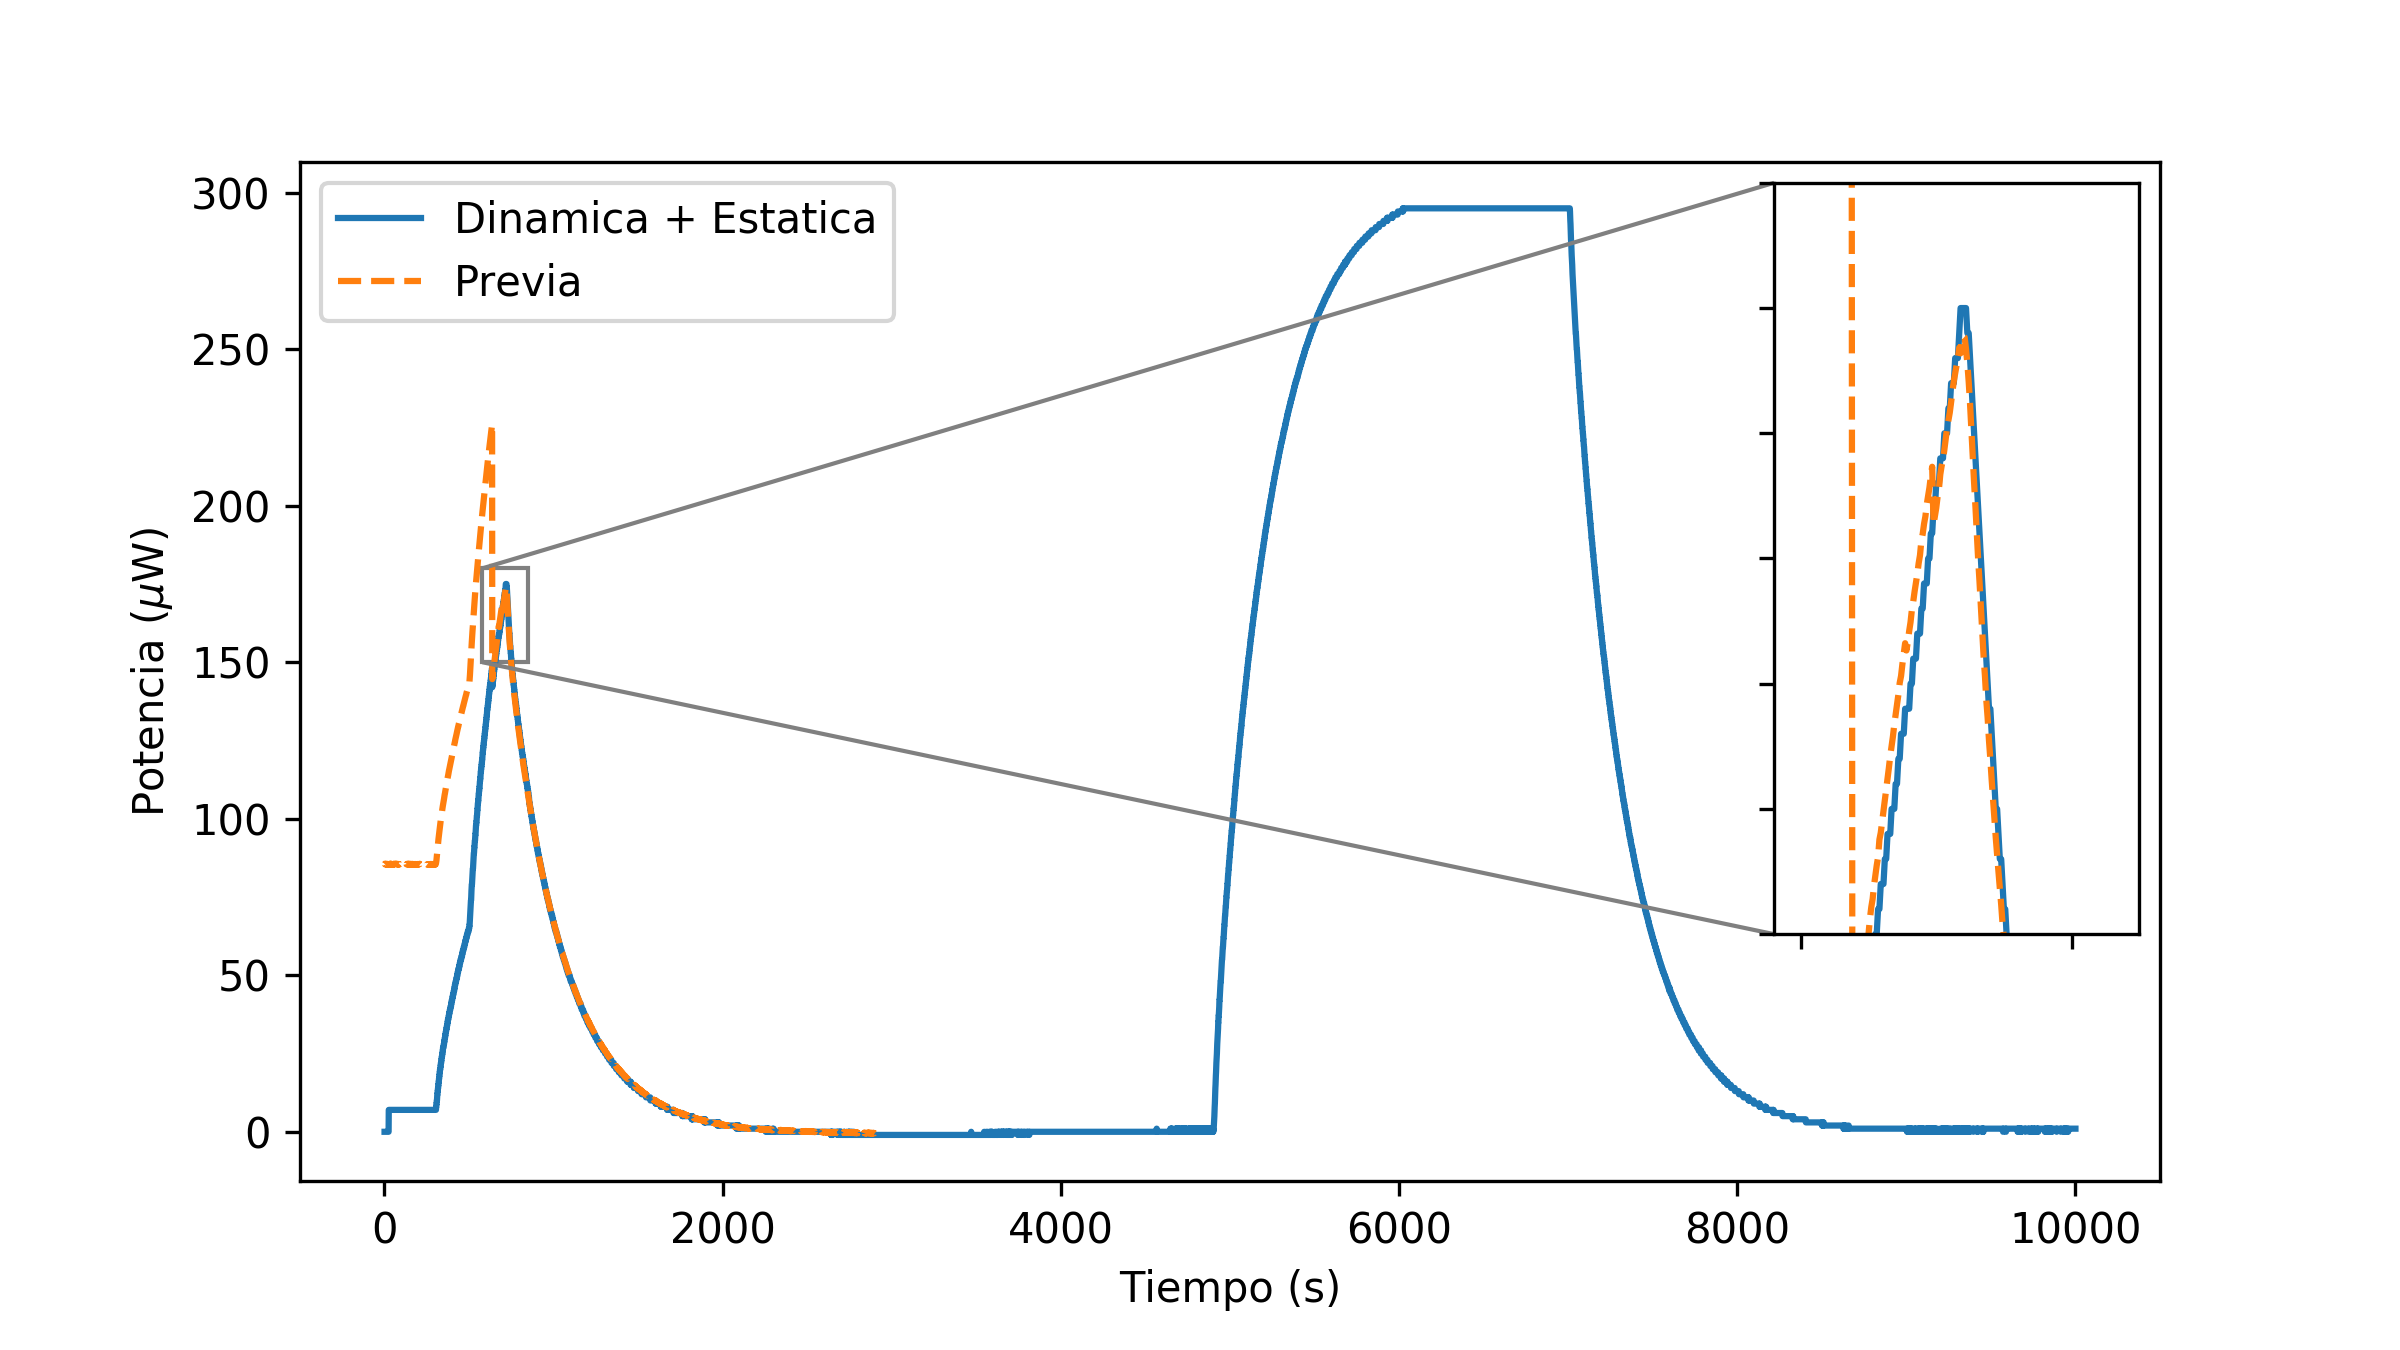
\includegraphics[width=\linewidth]{../Data/ElectricalCalibrations/Both}
		\caption{Calibraciones dinámica y estática que muestran el correcto funcionamiento del calorímetro.}
		\label{fig: dynamicStatic}
	\end{figure}
	 
% !TeX spellcheck = es_ES
% Chapter 1

%\chapter{Chapter Title Here} % Main chapter title
%
%\label{Chapter1} % For referencing the chapter elsewhere, use \ref{Chapter1} 

%----------------------------------------------------------------------------------------

% Define some commands to keep the formatting separated from the content 
%\newcommand{\keyword}[1]{\textit{#1}}
%\newcommand{\tabhead}[1]{\textbf{#1}}
%\newcommand{\code}[1]{\texttt{#1}}
%\newcommand{\file}[1]{\texttt{\bfseries#1}}
%\newcommand{\option}[1]{\texttt{\itshape#1}}

%----------------------------------------------------------------------------------------

\chapter{Calibraci\'on Qu\'imica}\label{ch: chemical}
	La calibraci\'on qu\'imica consiste en contrastar las propiedades termodin\'amicas de un sistema qu\'imico, obtenidas usando el calor\'imetro con aquellas reportadas en la literatura, esto es de vital importancia dado que las calibraciones el\'ectricas con frecuencia no transfieren a la celda el 100 \% de la potencia aplicada, as\'i mismo la distribuci\'on de calor puede ser considerablemente distinta a la de una reacci\'on. Dos sistemas qu\'imicos fueron usados para la realizaci\'on de la calibraci\'on qu\'imica: la reacci\'on del \'acido clorhidrico con bicarbonato de potasio, y la disoluci\'on de 1-propanol en agua. Estas sistemas hacen uso de reactivos de f\'acil acceso, han sido estudiados previamente en los procesos de calibraci\'on de equipos calorim\'etricos, como el calor\'imetro de titulaci\'on NanoITC de \textit{TA Instruments} con el que cuenta el grupo de \groupname{} \cite{demarse2011calibration, adao2012chemical, nanoitc}. En el caso de la neutralizaci\'on del \'acido clorh\'idrico es posible obtener par\'ametros termodin\'amicos como la entalp\'ia de reacci\'on, entrop\'ia y energ\'ia libre de Gibbs.

\section{Sistema de inyecci\'on}
	El sistema de inyecci\'on consiste en un motor de pasos acoplado a un tornillo de precisión, el cual controla el desplazamiento del émbolo de la jeringa de inyección. El fluido saliente de la jeringa se desvía usando una manguera de cromatografía líquida de acero inoxidable, el cual se conecta en el otro extremo a un canal que lleva el fluido hasta la celda de medición (\autoref{fig: sistemaInyeccion}).
	
	\begin{figure}[h]
		\centering
		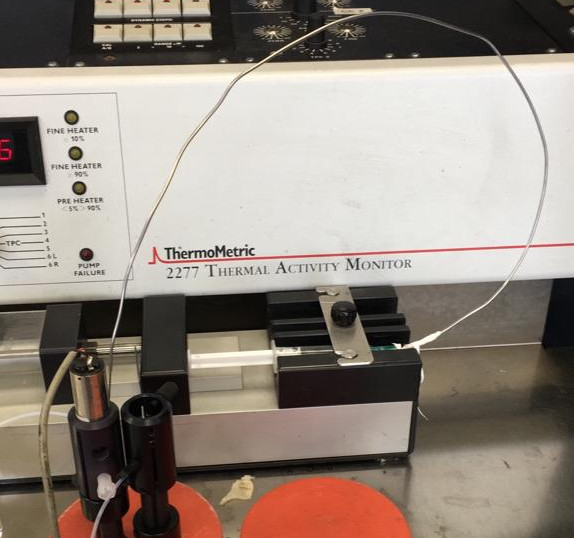
\includegraphics[width=0.6\linewidth]{Figures/sistemaInyeccion}
		
		\caption{Sistema de inyección construido como alternativa al uso de las canulas.}
		\label{fig: sistemaInyeccion}
	\end{figure}
	
	Tanto la aguja de la jeringa como la manguera de cromatografía, corresponden con una alternativa para ingresar el fluido hasta la celda que difiere del mecanismo original en los volúmenes usados y el tipo de jeringas. Originalmente, para introducir una sustancia en la celda se hace uso de una jeringa de vidrio Hammilton de 250 $\mu$L la cual cuenta con una canula soldada en la punta de esta. Al momento de realizar las calibraciones qu\'imicas, no se contaba con una jeringa de este tipo con la canula conectada, y a pesar que varios intentos fueron realizados para soldar la punta con la canula de oro y acero inoxidable, no fue posible juntar las mismas, en parte dado que el diámetro de la canula es considerablemente pequeño, siendo difícil de ver a simple vista. Lo anterior tiene consideraciones especiales, pues los diámetros de la jeringa y la manguera no son compatibles, por lo cual se hace necesario usar cinta de teflón para evitar al máximo fugas en el sistema. Otro aspecto a considerar es que el volumen interno de la manguera cromatogr\'afica es mucho mayor al de la canula, por lo cual se debe tener especial cuidado por los volúmenes introducidos, pues no se debe exceder la capacidad de 4 mL de la celda.
	
	\subsection{Control por automatizado}\label{ssec: jeringa}
	Para acceder al control de la jeringa, en el menú superior: \texttt{System > Auxiliary > Pump}. En el momento se cuenta con un único agitador para la celda, por lo cual sólo se encuentra instalado uno de los controladores de jeringa tipo \texttt{Lund}, por esta razón el sistema debe detectar automáticamente únicamente el primer controlador (\texttt{Installed = yes}). La configuración de una jeringa consiste en escribir el volumen de esta (\texttt{Syringe volume}), la velocidad con la que se quiere mover el émbolo (\texttt{Plunger speed}), su longitud (\texttt{Syringe length}) y el volumen de inyección (\texttt{Dispense volume}).
	
	\begin{figure}[h]
		\centering
		\begin{subfigure}[b]{0.4\textwidth}
			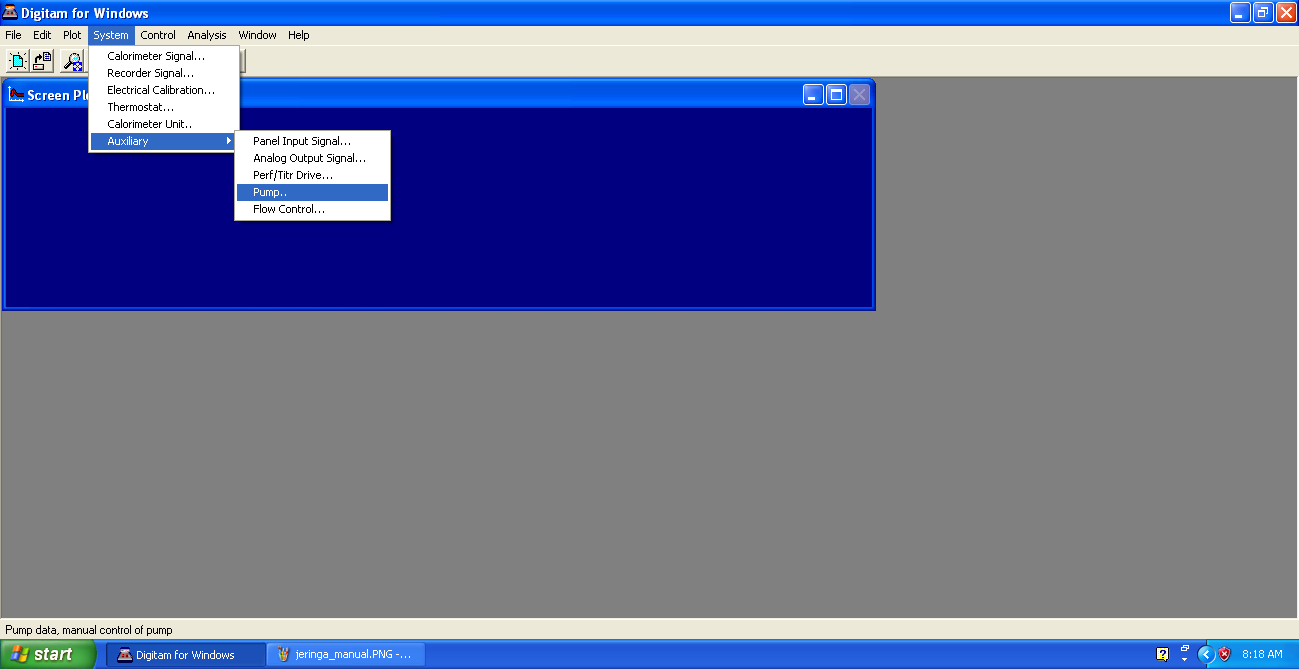
\includegraphics[width=\linewidth]{Figures/jeringa_menu}
			\caption{Ingreso al menú.}
			\label{fig: menuJeringa}
		\end{subfigure}
		\begin{subfigure}[b]{0.55\textwidth}
			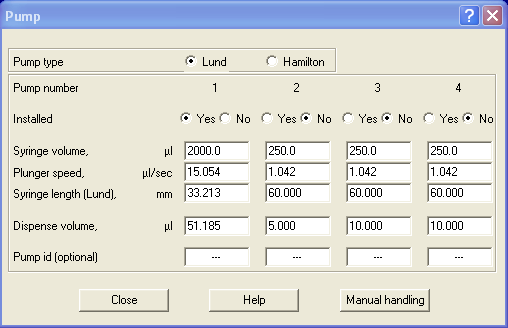
\includegraphics[width=\linewidth]{Figures/jeringa_config}
			\caption{Menú de configuración}
			\label{fig: configJeringa}
		\end{subfigure}
		\caption{Configuración de la jeringa en Digitam.}
	\end{figure}
	\newpage
	
	Una vez se encuentra configurada la jeringa, es posible usarla de dos maneras distintas. Por un lado se tiene el modo manual, donde el usuario tiene la posibilidad de avanzar rápidamente (\texttt{Fast forward}), por ejemplo para disminuir al distancia entre el émbolo y el pistón. En este modo, también es posible aumentar esta distancia (\texttt{Fast backward}), avanzar un milímetro (\texttt{One milimeter forward}) y moverse la distancia requerida para que la jeringa dispense el volumen por inyección (\texttt{Dispense}). Por otro lado, el control manual resulta útil antes de iniciar un experimento, pues con frecuencia será necesario ajustar la distancia entre el pistón y el émbolo para que haya contacto. Además, en el caso de ser requerida una calibración de la jeringa es posible usar el botón de dispensar para determinar si el volumen dispensado corresponde con el volumen configurado.
	\begin{figure}[h]
		\centering
		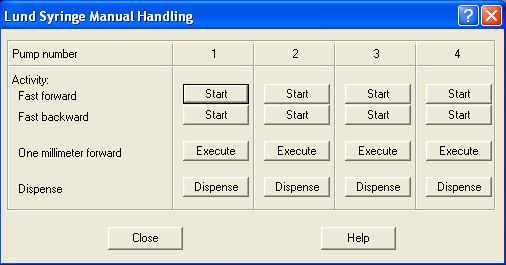
\includegraphics[width=0.5\linewidth]{Figures/jeringa_manual}
		\caption{Panel del uso manual del controlador de la jeringa.}
		\label{fig: manualJeringa}
	\end{figure}
	
	El modo automático se configura al momento de definir el método del experimento. Para esto es necesario expandir la opción de \texttt{Auxiliary system} en el panel izquierdo del menú y seleccionar el  \texttt{Pump and flow control}. Se debe tener en cuenta la sección del experimento que se está configurando. En el caso de la \autoref{fig: autoJeringa}, sólo existe la sección de \texttt{Baseline}, en esta sección se busca realizar 20 inyecciones, cada una con el volumen de dispensación y velocidad configurados en la \autoref{fig: configJeringa}, y 300 segundos de espera entre cada inyección.
	\begin{figure}[h]
		\centering
		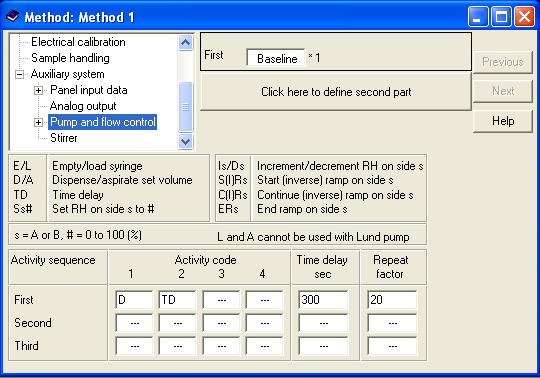
\includegraphics[width=0.5\linewidth]{Figures/jeringa_experimento}
		\caption{Panel de configuración de la jeringa en modo automático.}
		\label{fig: autoJeringa}
	\end{figure}
	
	\subsection{Calibraci\'on de la jeringa}
	Si bien el volumen de una jeringa es bien conocido, la longitud del émbolo es un parámetro que con frecuencia no se encuentra fácilmente. El controlador de la jeringa depende de este valor para relacionar la longitud que debe expandir el pistón para dispensar el volumen $V_d$. Por esta razón, para determinar la longitud correcta de la jeringa que debe ser configurada, se usaron distintos valores de esta y se midió la masa de agua tipo 1 desplazada, para cada valor de longitud se tomaron 3 medidas, los cuales se muestran en la \autoref{tb: syringeCal}.
	\begin{table}[h]
		\centering
		\caption{Masa dispensada por la jeringa usando diferentes longitudes y un $V_d = 100.000$ $\mu$L}
		\small
		\begin{tabular}{p{1.7cm}|p{1.3cm}p{1.3cm}p{1.3cm}|p{2cm}p{2cm}}
			\hline
			\textbf{Longitud (mm)} &  \textbf{Masa 1 (g)} &  \textbf{Masa 2} (g) &  \textbf{Masa 3 (g)} &  \textbf{Promedio (g)} & \textbf{Desviacion (g)} \\
			\hline
			28,000 & 0,08194 & 0,08196 & 0,08262 & 0,0822 & 0,0004 \\
			29,000 & 0,08573 & 0,08673 & 0,08648 & 0,0863 & 0,0005 \\
			30,000 & 0,09003 & 0,08884 & 0,08970 & 0,0895 & 0,0006 \\
			31,000 & 0,09270 & 0,09322 & 0,09263 & 0,0928 & 0,0003 \\
			32,000 & 0,09551 & 0,09536 & 0,09538 & 0,0954 & 0,0001 \\
			33,000 & 0,09895 & 0,09825 & 0,09870 & 0,0986 & 0,0004 \\
			34,000 & 0,10172 & 0,10176 & 0,10137 & 0,1016 & 0,0002 \\
			35,000 & 0,10409 & 0,10318 & 0,10422 & 0,1038 & 0,0006 \\
			36,000 & 0,10679 & 0,10593 & 0,10757 & 0,1068 & 0,0008 \\
			37,000 & 0,10958 & 0,11015 & 0,10993 & 0,1099 & 0,0003 \\
			38,000 & 0,11384 & 0,11327 & 0,11360 & 0,1136 & 0,0003 \\
			\hline
		\end{tabular}
		\label{tb: syringeCal}
	\end{table}
	
	\begin{figure}[h!]
		\centering
		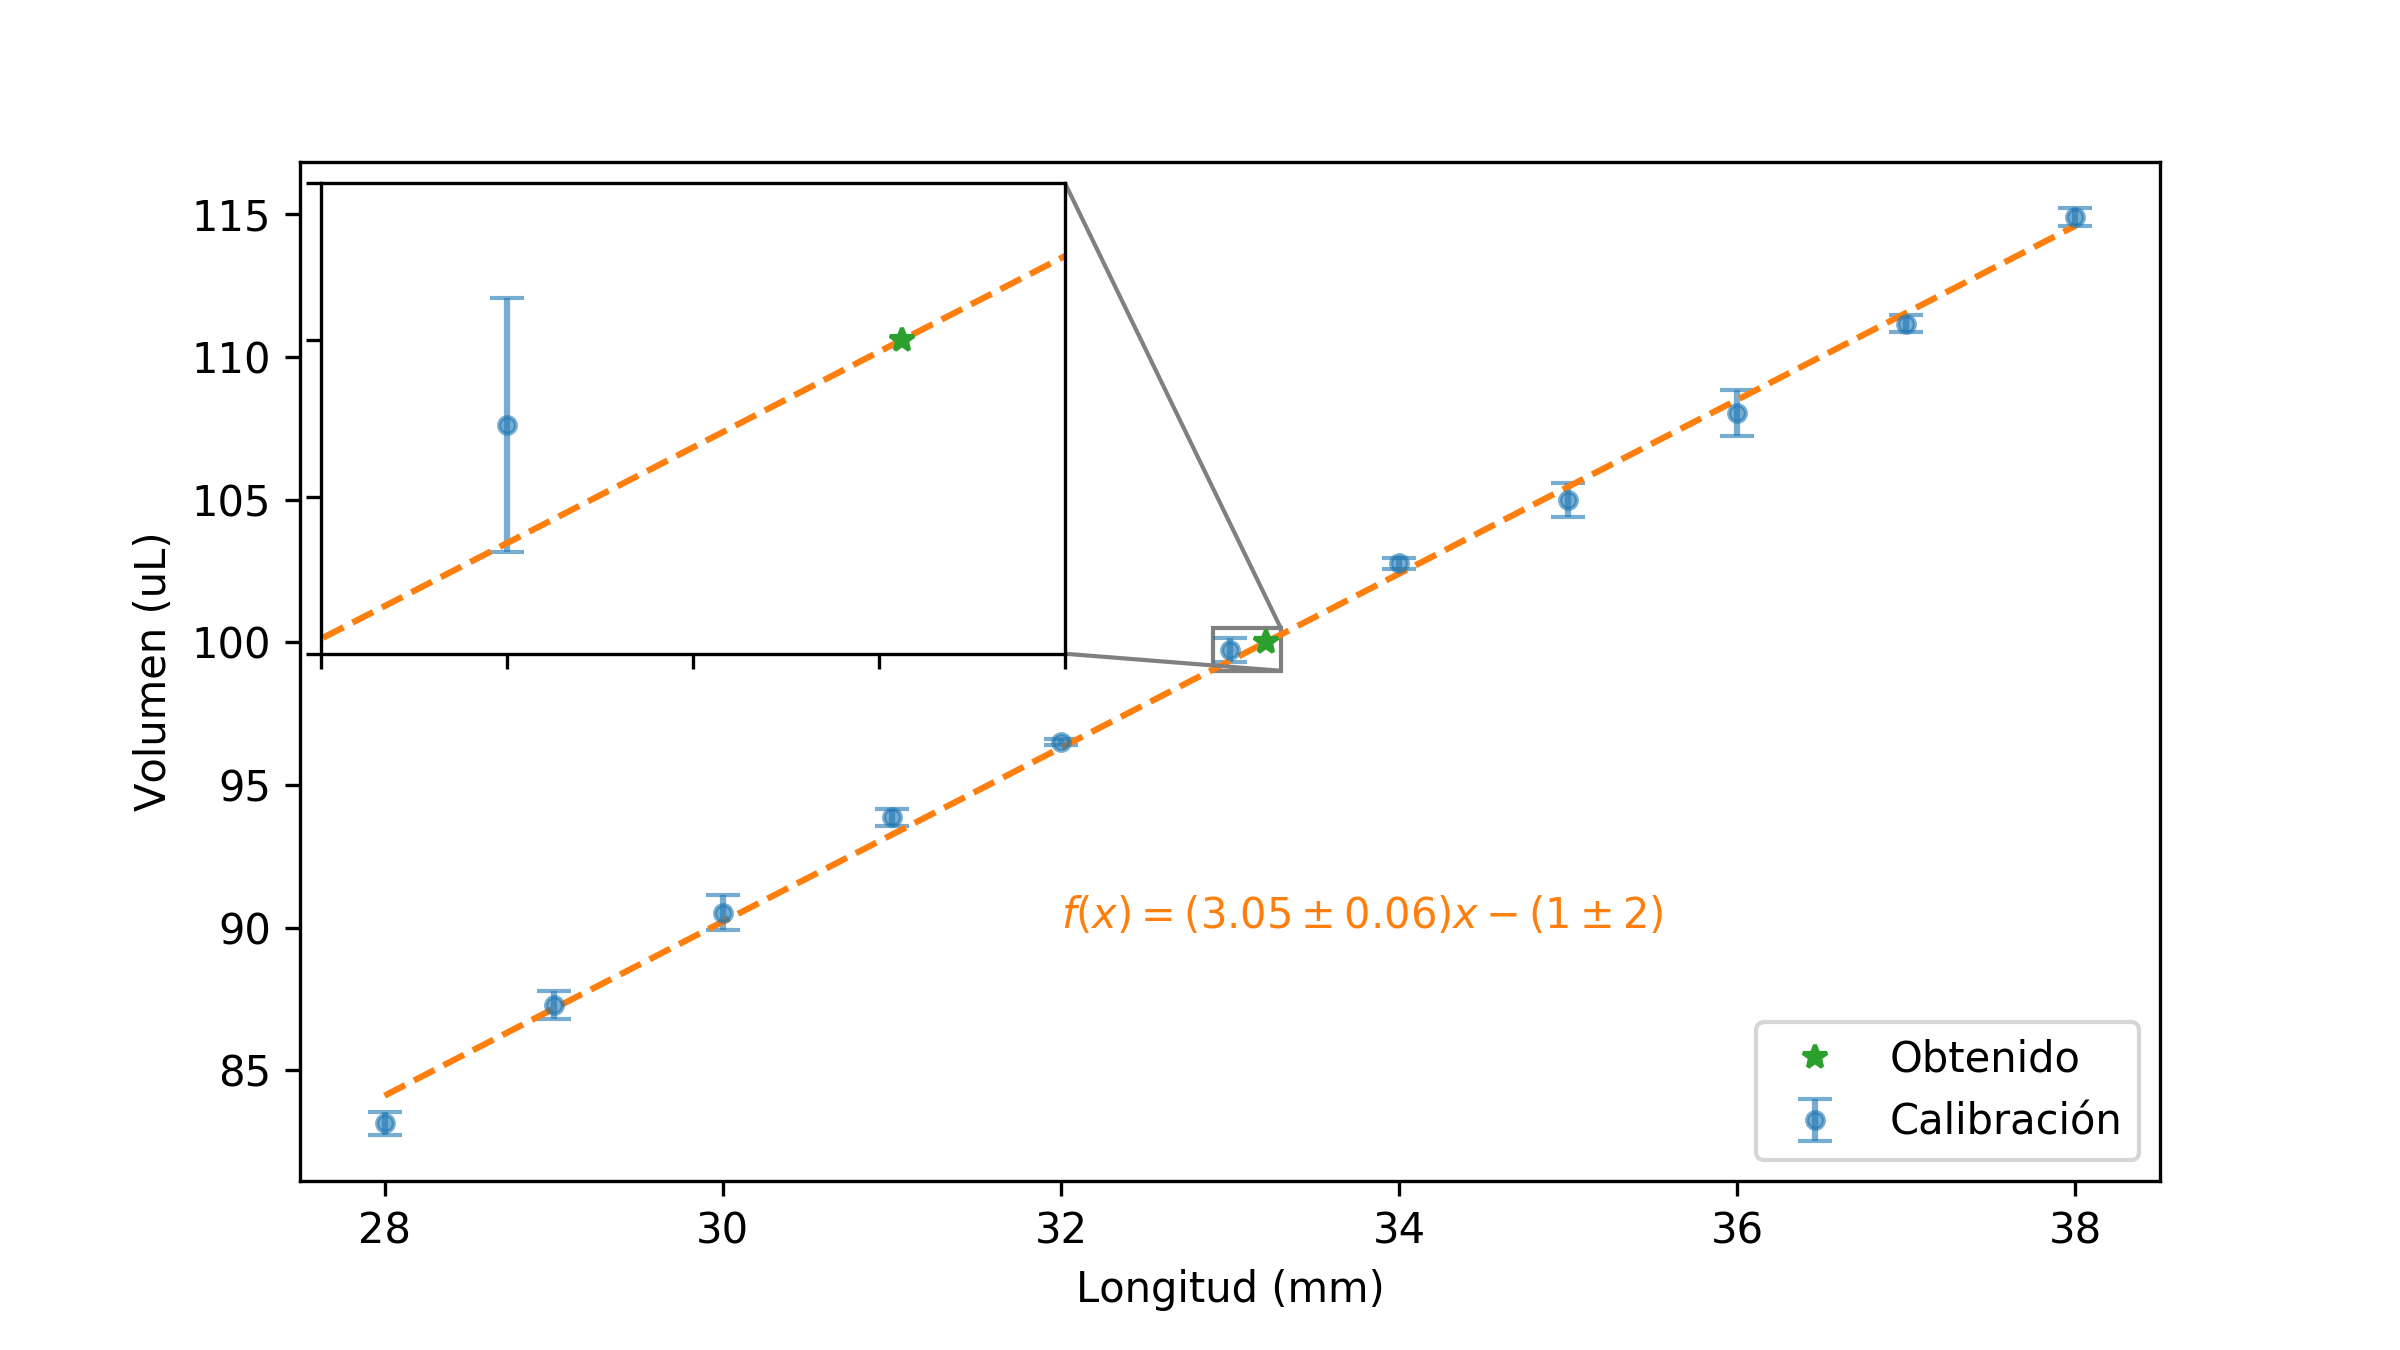
\includegraphics[width=\linewidth]{../Data/Syringe/syringe_cal.png}
		\caption{Curva de calibraci\'on de la jeringa usada.}
		\label{fig: syringeCal}
	\end{figure}
	
	Con el termómetro de mercurio usado en la calibración térmica de los sensores de temperatura se midió la temperatura del agua usada en la calibración de la jeringa, dando un valor de 17.7 $^\circ$C. El densimetro usado en la \autoref{sec: soluciones} fue configurado para realizar una lectura a esta misma temperatura, con lo cual se obtuvo un valor de densidad de 0.998679 g/cm$^3$. Con esta información, es posible construir una curva que permite inferir la configuración a usar de la jeringa, la cual, junto con el valor escogido, se muestran en la \autoref{fig: syringeCal}. Para un volumen de dispensación de 100 $\mu$L, se obtuvo una longitud de 33,213 mm.	

\section{Calibraci\'on 1-propanol y agua}
	La disoluci\'on de 1-propanol en agua constituye otro m\'etodo reportado por varios autores para realizar una calibraci\'on qu\'imica \cite{briggner1991test, nanoitc, demarse2011calibration, adao2012chemical}. Un gr\'afico de energ\'ia transferida en forma de calor en funci\'on del n\'umero de inyecciones o el volumen total inyectado, debe seguir una tendencia lineal \cite{demarse2011calibration, nanoitc, adao2012chemical}. 
	
\subsection{Preparaci\'on de la soluci\'on 3 \%}
	Para conocer la masa de agua que se debe adicionar para obtener una soluci\'on con concentraci\'on final $P$ en porcentaje masa, a partir de una masa $m'_\text{total}$ de una soluci\'on con concentraci\'on $P'$ conocida, se usa la siguiente ecuaci\'on:
	\begin{equation}\label{eq: massConcentration}
		P = \dfrac{m_\text{propanol}}{m_\text{total}} = \dfrac{P'm'_\text{total}}{m_\text{\ce{H2O}} + m'_\text{total}} \longrightarrow m_\text{\ce{H2O}} = \left(\dfrac{P'}{P} -1\right)m'_\text{total}
	\end{equation}
	
	Para un gramo de 1-propanal (99,8 \% LiChrosolv para cromatograf\'ia l\'iquida), fueron medidos 33,6457 g de agua tipo 1 previamente desgasificada de manera an\'aloga a las soluciones de HCl y \ce{KHCO3}. Sobre el agua se adicionaron 1.0290 g de 1-propanol, para obtener una soluci\'on final de 1-propanol de 2,96 \%, cuya densidad a 20 \grad{} es 0.993487 g/cm$^3$.
	
	\subsection{Realizaci\'on de los experimentos}\label{sec: method}
	El m\'etodo experimental est\'a dividido en cuatro partes:
	\begin{enumerate}
		\item \textbf{Pause}: En la etapa inicial del experimento se busca medir el estado de la línea base por 120 minutos consecutivos.
		\item \textbf{Baseline}: Luego de tener datos sobre el estado sin perturbar del sistema, se realiza una calibración dinámica para obtener un ajuste fino de los parámetros de ganancia y nivel del cero de la señal. 
		\item \textbf{Pause:} En este punto se realiza una calibraci\'on est\'atica para confirmar que la calibraci\'on din\'amica fue correcta. Para esto, se aplican 300 $\mu$W sobre la celda por 30 minutos, posteriormente se retira la potencia y se esperan 50 minutos para la estabilizaci\'on de la linea base.
		\item \textbf{Main:} Una vez estabilizada la linea base, se realizan 30 inyecciones sucesivas con 10 minutos de espera entre cada inyecci\'on, la velocidad de inyecci\'on es de 50,018 $\mu/s$ y el volumen de inyecci\'on es de 51,185 $\mu$L.
	\end{enumerate}
	
	Con esta soluci\'on tres experimentos fueron realizados, las cantidades usadas en cada uno de ellos se muestra en la \autoref{tb: propanolQuantity}.
	
	\begin{table}[h]
		\centering
		\caption{Experimentos realizados con la soluci\'on 2,96\% de 1-propanol.}
		\begin{tabular}{cccc}
			\hline
			\textbf{Experimento} & \textbf{Masa \ce{H2O} (g)} & \textbf{\# inyecciones} & \textbf{Volumen inyectado ($\mu$L)}\\
			\hline
			1 & 2,41273 & 27 & 27 * 51,185 \\
			2 & 2,49389 & 1 & 1382,0 \\
			3 & 2,56668 & 1 & 1382,0 \\
			\hline
		\end{tabular}
		\label{tb: propanolQuantity}
	\end{table}
	
	%	Ad\~ao y colaboradores proponen tres m\'etodos para calcular la entalp\'ia de mezcla, todos los cuales hacen uso de inyecciones de 1-propanol en agua. En el primer m\'etodo, se calcula el promedio de las entalp\'ias indiviales por inyecci\'on, en el segundo se realiza una regresi\'on lineal donde en el eje $y$ se grafica la entalp\'ia de diluci\'on en funci\'on de la concentraci\'on, y el tercero calcula la entalp\'ia a partir de los coeficientes de interacci\'on ent\'alpicos \cite{adao2012chemical}. Ad\~ao y colaboradores estudian la dependencia de estos valores con la concentraci\'on las cuales se encuentran entre 2 \%, 5 \% y 
	%	
	%	
	%	 concentraci\'on realizan inyecciones con vol\'umenes entre 2 y 5 $\mu$L de soluciones de 1-propanol con concentraciones de 2 \%, 5 \% y 10 \% en fracci\'on de masa. Inicialmente, y dada la experiencia con la reacci\'on de neutralizaci\'on se procedi\'o a realizar una calibraci\'on qu\'imica adicionando 51,185 $\mu$L de 1-propanol por inyecci\'on (pureza 99.8 \% LiChrosolv para cromatograf\'ia l\'iquida) a la celda de medici\'on que contaba con 1.6235 g de agua tipo 1.
	%	\begin{figure}[h]
	%		\centering
	%		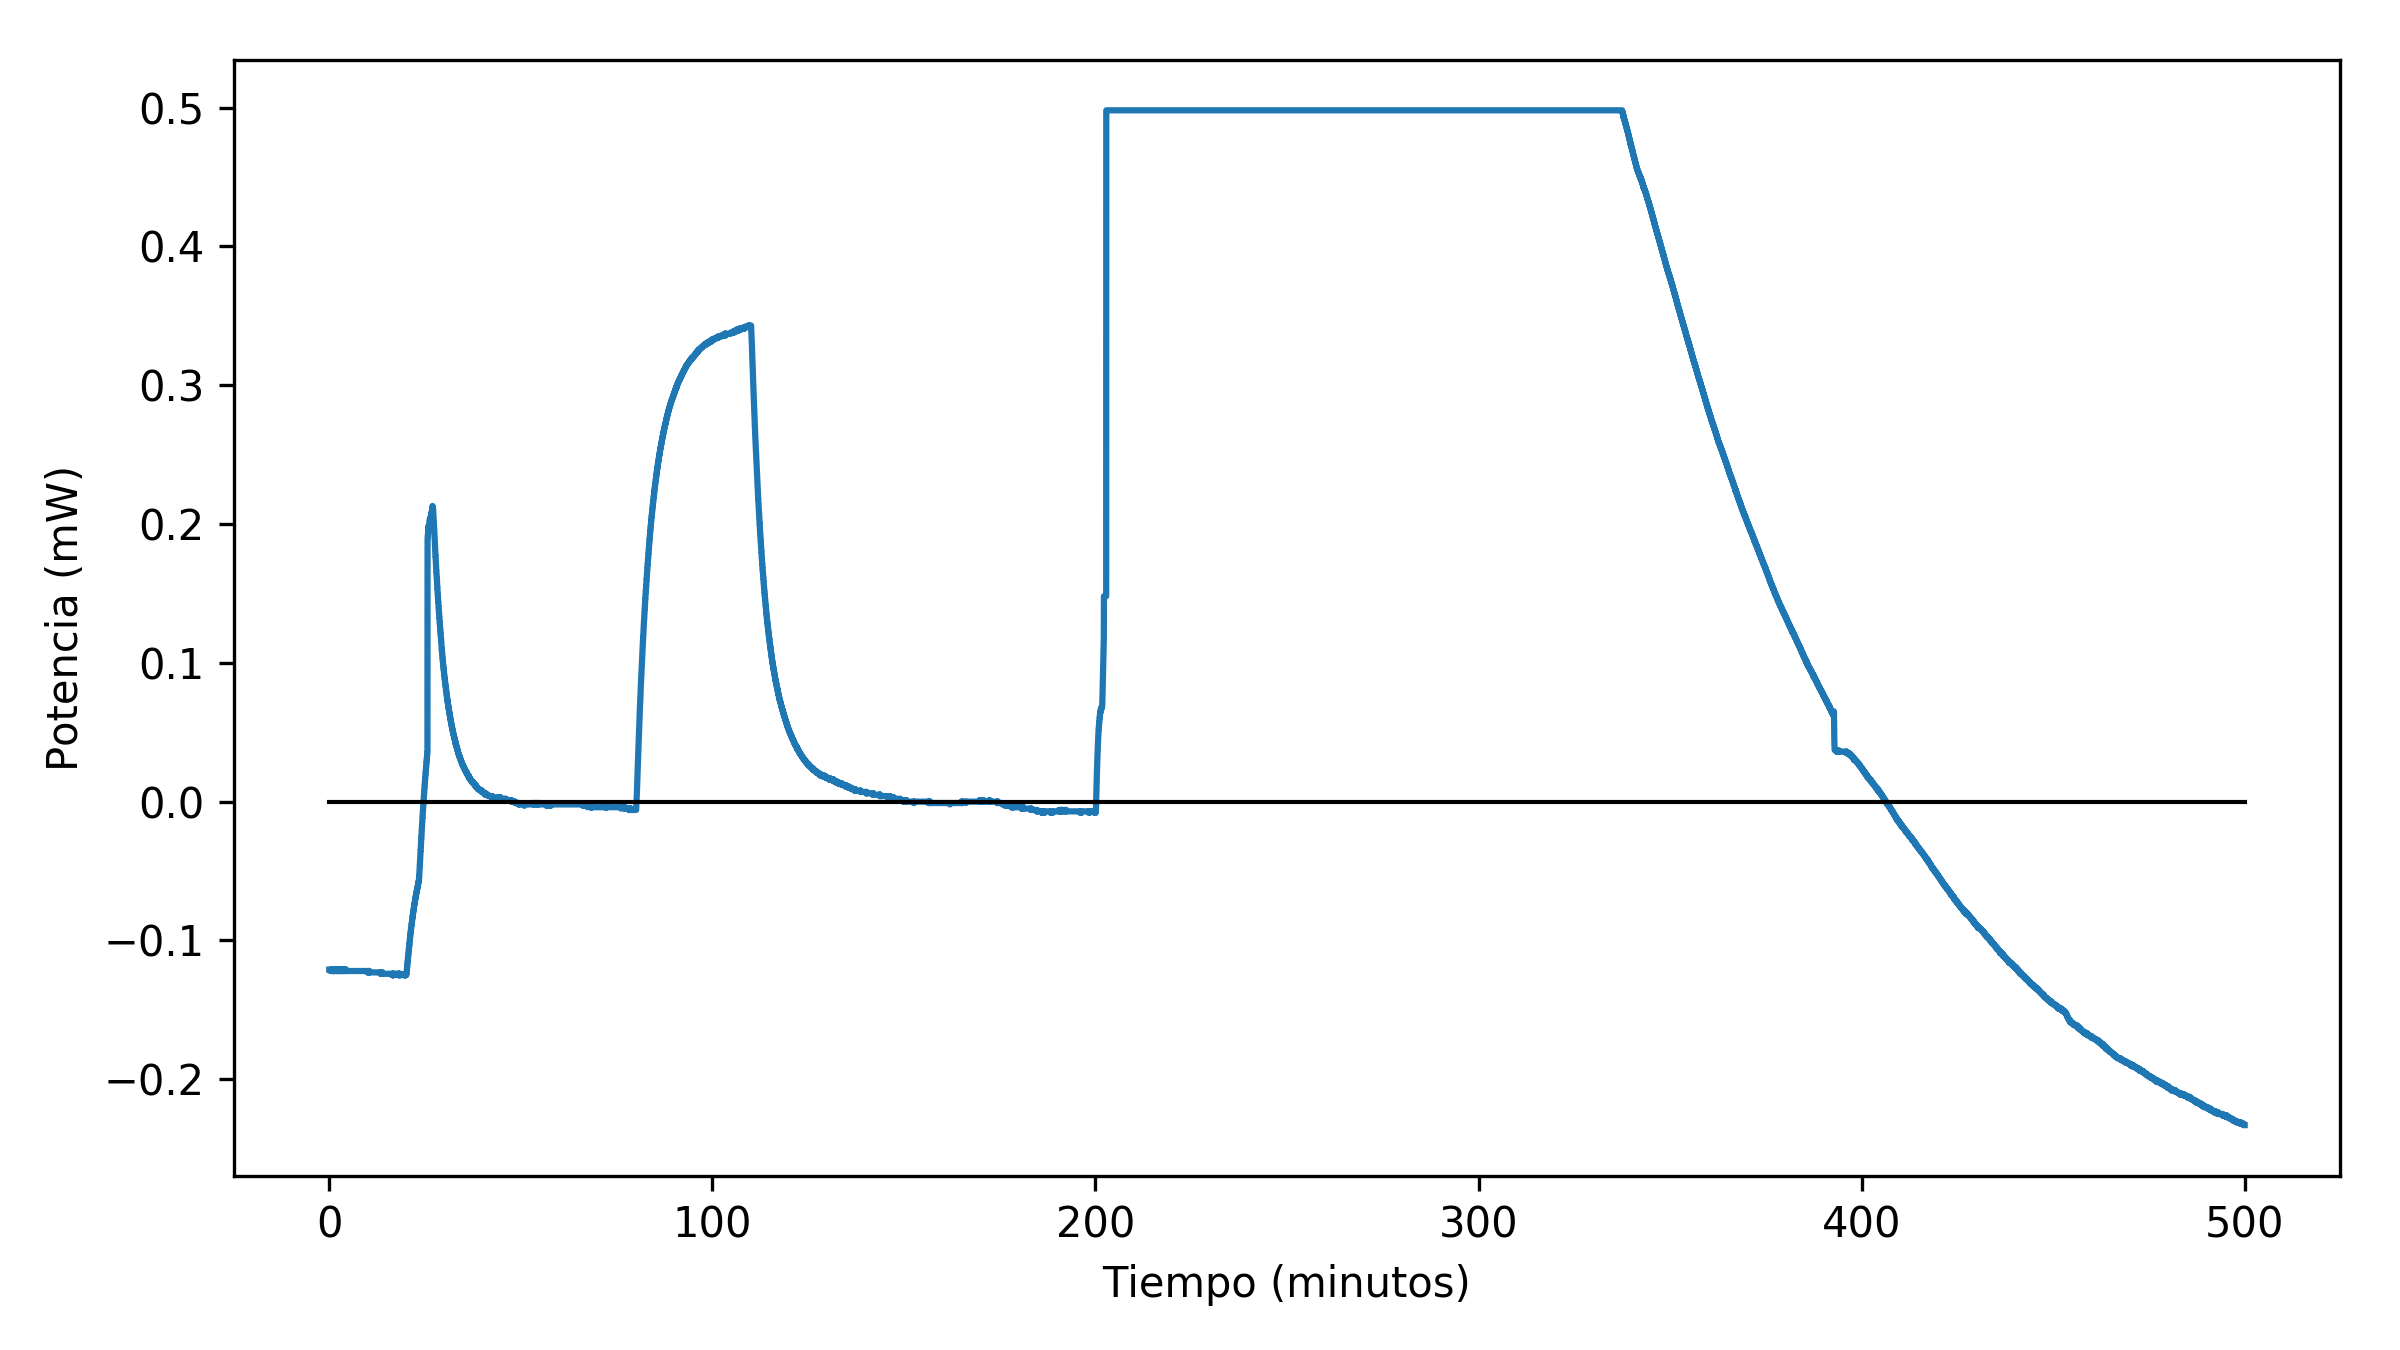
\includegraphics[width=\linewidth]{../Data/ChemicalCalibrations/concentratedPropanol}
	%		\caption{Resultados obtenidos para la mezcla de agua con 1-propanol concentrado, las inyecciones tienen lugar a partir del minuto 200.}
	%		\label{fig: CPropanolResults}
	%	\end{figure}
	
	
	El m\'etodo experimental procedi\'o de la misma forma que en la \autoref{sec: method}, sin embargo como se muestra en la \autoref{fig: CPropanolResults}, luego de la primera inyecci\'on el sistema se satur\'o imposibilitando, nuevamente la cuantificaci\'on de la potencia generada. Una vez se determin\'o que el calor\'imetro hab\'ia detectado, pero no cuantificado la disoluci\'on, se procedi\'o preparar una soluci\'on 2,96 \% de 1-propanol. Para esto se disolvieron 1,0290 g de 1-propanol en 33.6457 g de agua, y su densidad fue de un valor de 0.993487 g/cm$^{3}$. Con el objetivo de limitar el efecto del sistema de inyecci\'on sobre las potencias registradas, para este experimento se realizaron 30 inyecciones con 1 minuto de espera entre cada una de ellas, adem\'as de ignorar la calibraci\'on est\'atica, pues hab\'ia sido realizada previamente. Los resultados se muestra en la \autoref{fig: singleInjection}, para realizar la integral se toman en cuenta el estado del calor\'imetro antes y despu\'es de las inyecciones, a partir de estas se obtiene la linea base durante las inyecciones (l\'inea naranja). Posteriormente, se realiza la resta de la se\~nal de potencia con la linea base para obtener que esta se encuentre justo sobre el cero (l\'inea verde), y finalmente se integran los datos num\'ericamente usando la regla del trapecio \cite{landau2008survey} implementado en la librer\'ia \texttt{numpy} de Python \cite{walt2011numpy}.
	
	\begin{figure}[h]
		\centering
		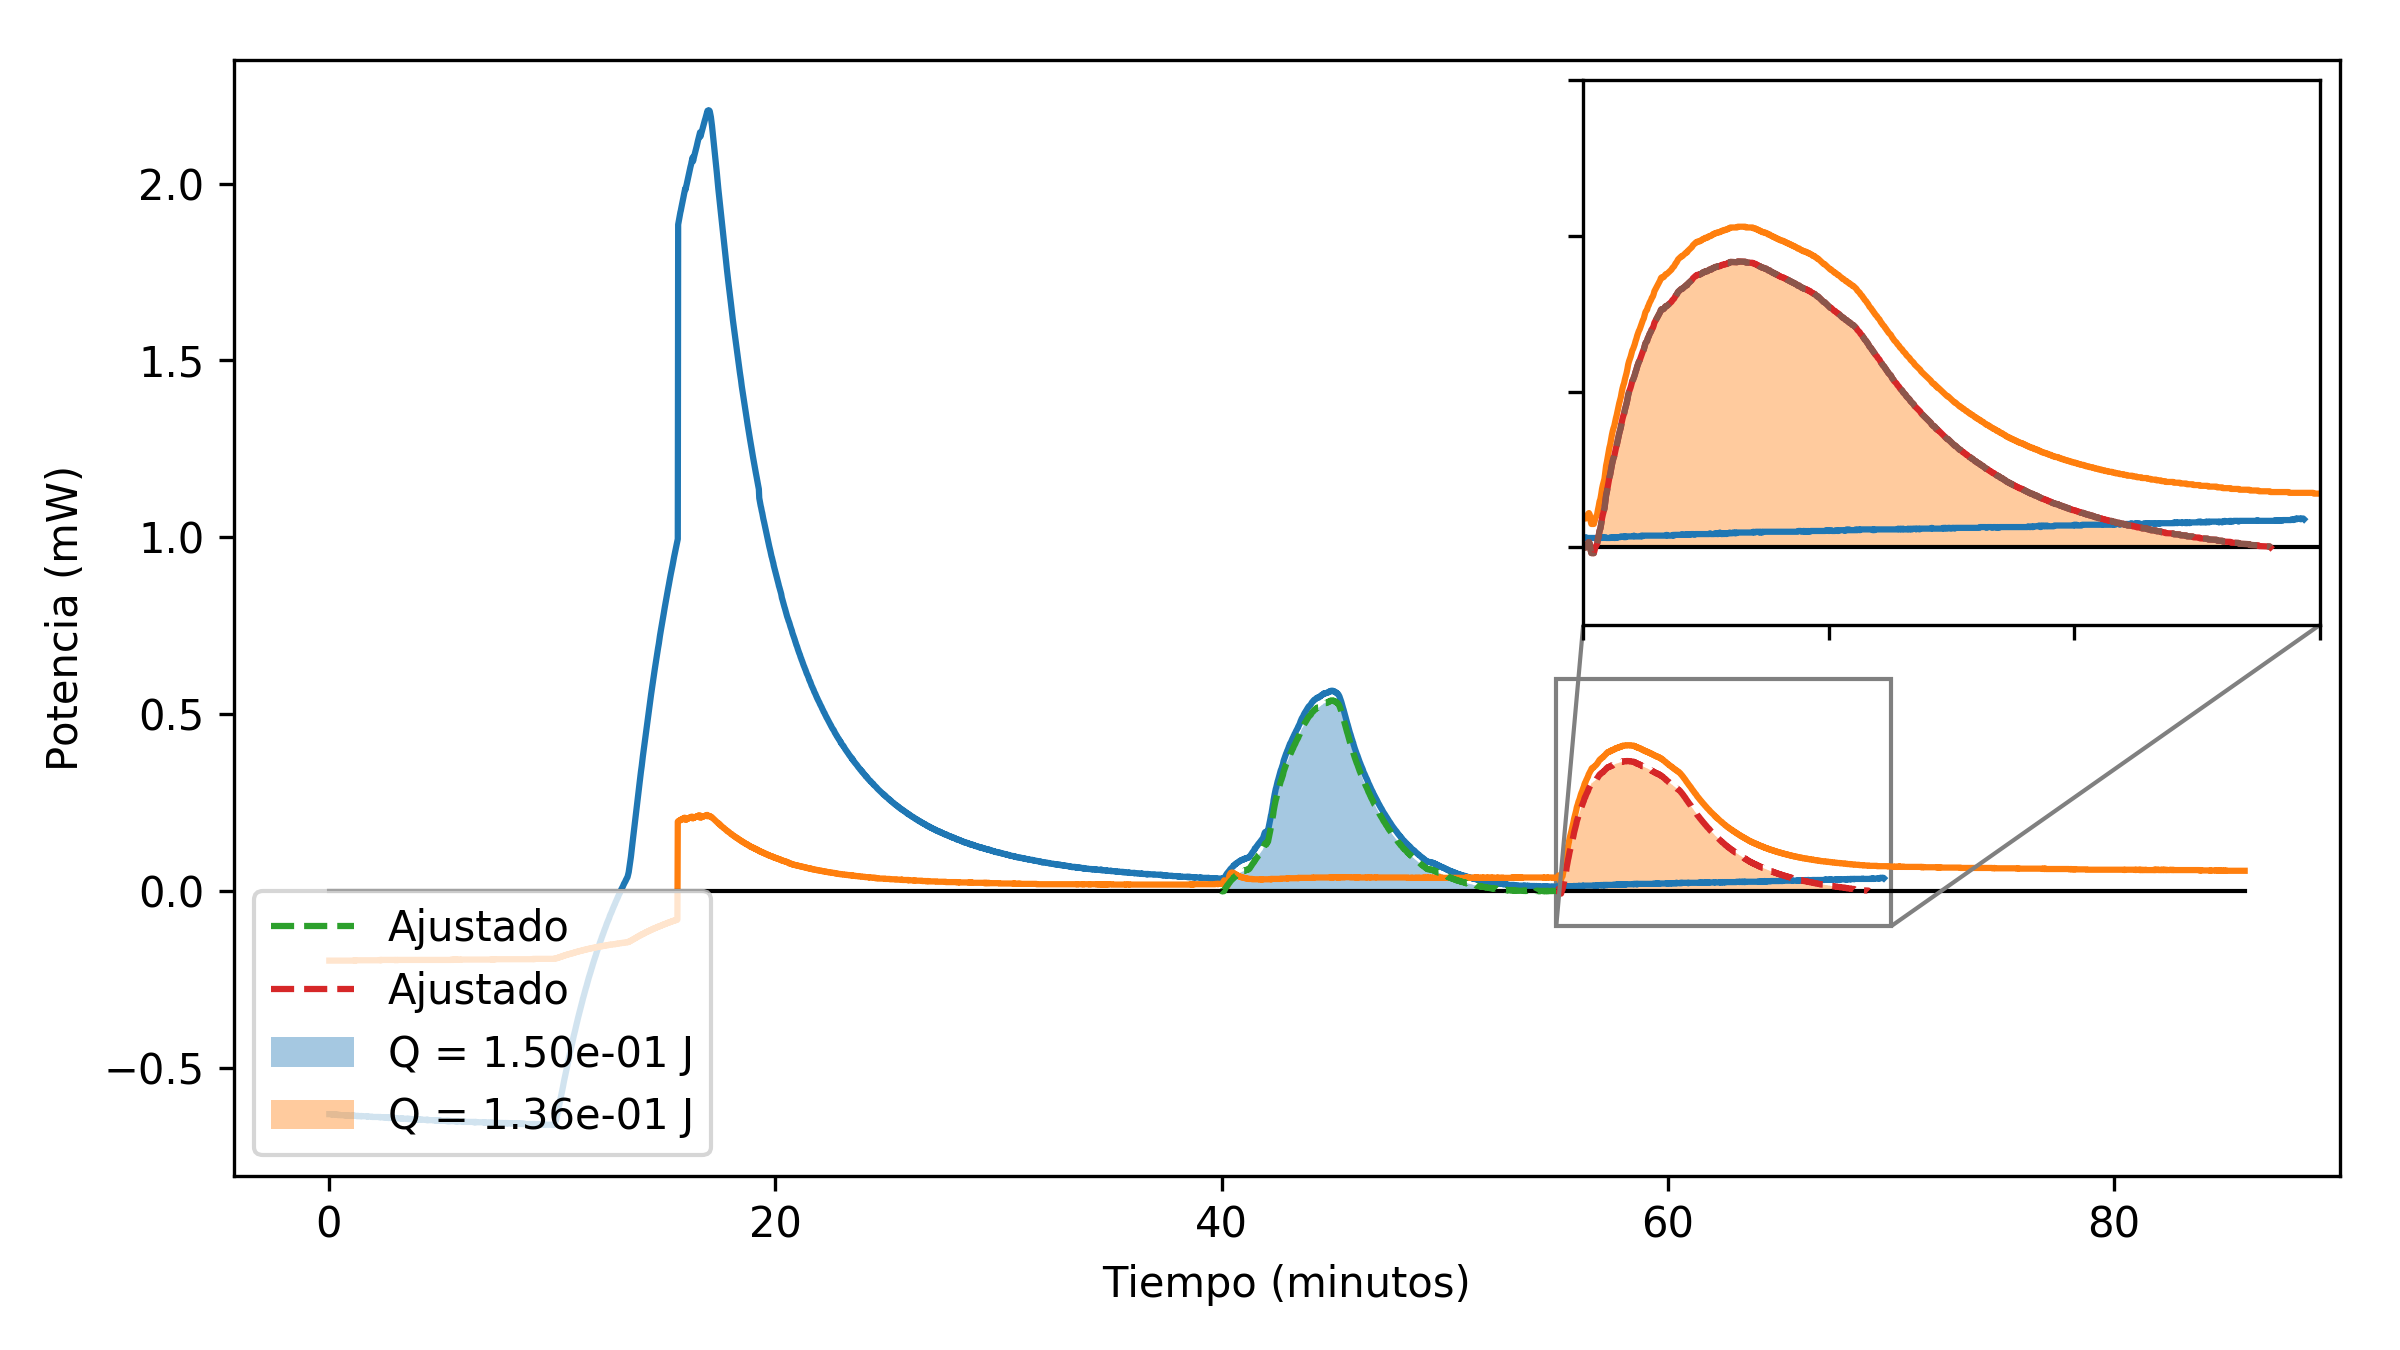
\includegraphics[width=\linewidth]{../Data/ChemicalCalibrations/singlePropanol}
		\caption{Resultados obtenidos para la mezcla de agua con 1-propanol 2,96\%.}
		\label{fig: singleInjection}
	\end{figure}
	
	\subsection{Resultados}
	La masa de 1-propanol contenida en cada volumen de inyecci\'on $V_\text{iny}$ est\'a determinada por:
	\begin{equation}
	m_p = \%m\rho V
	\end{equation}
	
	La energ\'ia transferida en forma de calor corresponde con: 149.2 mJ. Ahora, considerando la densidad de la soluci\'on y el volumen de inyecci\'on se tiene que por cada una se introducen:

\section{Calibraci\'on con HCl y \ce{KHCO3}}\label{sec: soluciones}
	Para la preparaci\'on de las soluciones de HCl y \ce{KHCO3} y 1-propanol, se hace uso de forma sistem\'atica de una balanza Ohaus Analytical Plus (AP250D) y un dens\'imetro Anton Paar DSA5000M. La balanza presenta incertidumbres de $1\times10^{-5}$ y $1\times10^{-4}$ g dependiendo del rango usado, para el primer caso la masa medida debe ser inferior a 80 g y en el segundo no puede superar los 250 g, siendo esta la capacidad máxima de la balanza. En el caso del densímetro, son necesarios volúmenes cercanos a 2 mL de una soluci\'on, con esto el equipo determina la densidad de la sustancia con incertidumbres de $1\times10^{-6}$ g/cm$^{-3}$ para una temperatura determinada por el usuario. Adem\'as, en el proceso de preparaci\'on se hace necesaria la toma de dos al\'icuotas de 30 $\mu$L y 170 $\mu$L, para el HCl y \ce{KHCO3} correspondientemente, por lo cual se usa una micropipeta pipet4u Performance con rango de 20 a 200 $\mu$L, que en el rango trabajado tienen precisiones superiores al 99.4 \% \cite{pipet4u}.
	
	\subsection{Soluci\'on de HCl 0.25 mM}
		Para determinar la concentraci\'on de una soluci\'on de 1,0 mL de HCl concentrado en 25,0 mL de agua tipo 1, se midi\'o la densidad de la soluci\'on, posteriormente, usando como referencia los datos reportados en la literatura, fue realizada una regresi\'on lineal que permiti\'o relacionar la concentraci\'on con la densidad de la soluci\'on $\rho$ \cite{perry2007perry}. De esta manera se estableci\'o el valor de la concentraci\'on en: $3.02 \pm 0.05$ \% (fracci\'on de masa $[w_t]$), donde la incertidumbre se obtiene de la pendiente ($m$) e intercepto ($b$) de la regresi\'on lineal que se muestra en la \autoref{fig: HCl_density}.
		\begin{equation}
			\delta [w_t] = \sqrt{\left(\dfrac{\rho-b}{m^2}\delta m\right)^2 + \left(\dfrac{\delta b}{m}\right)^2 + \left(\dfrac{\delta \rho}{m}\right)^2}
		\end{equation}
		\begin{figure}[h]
			\centering
			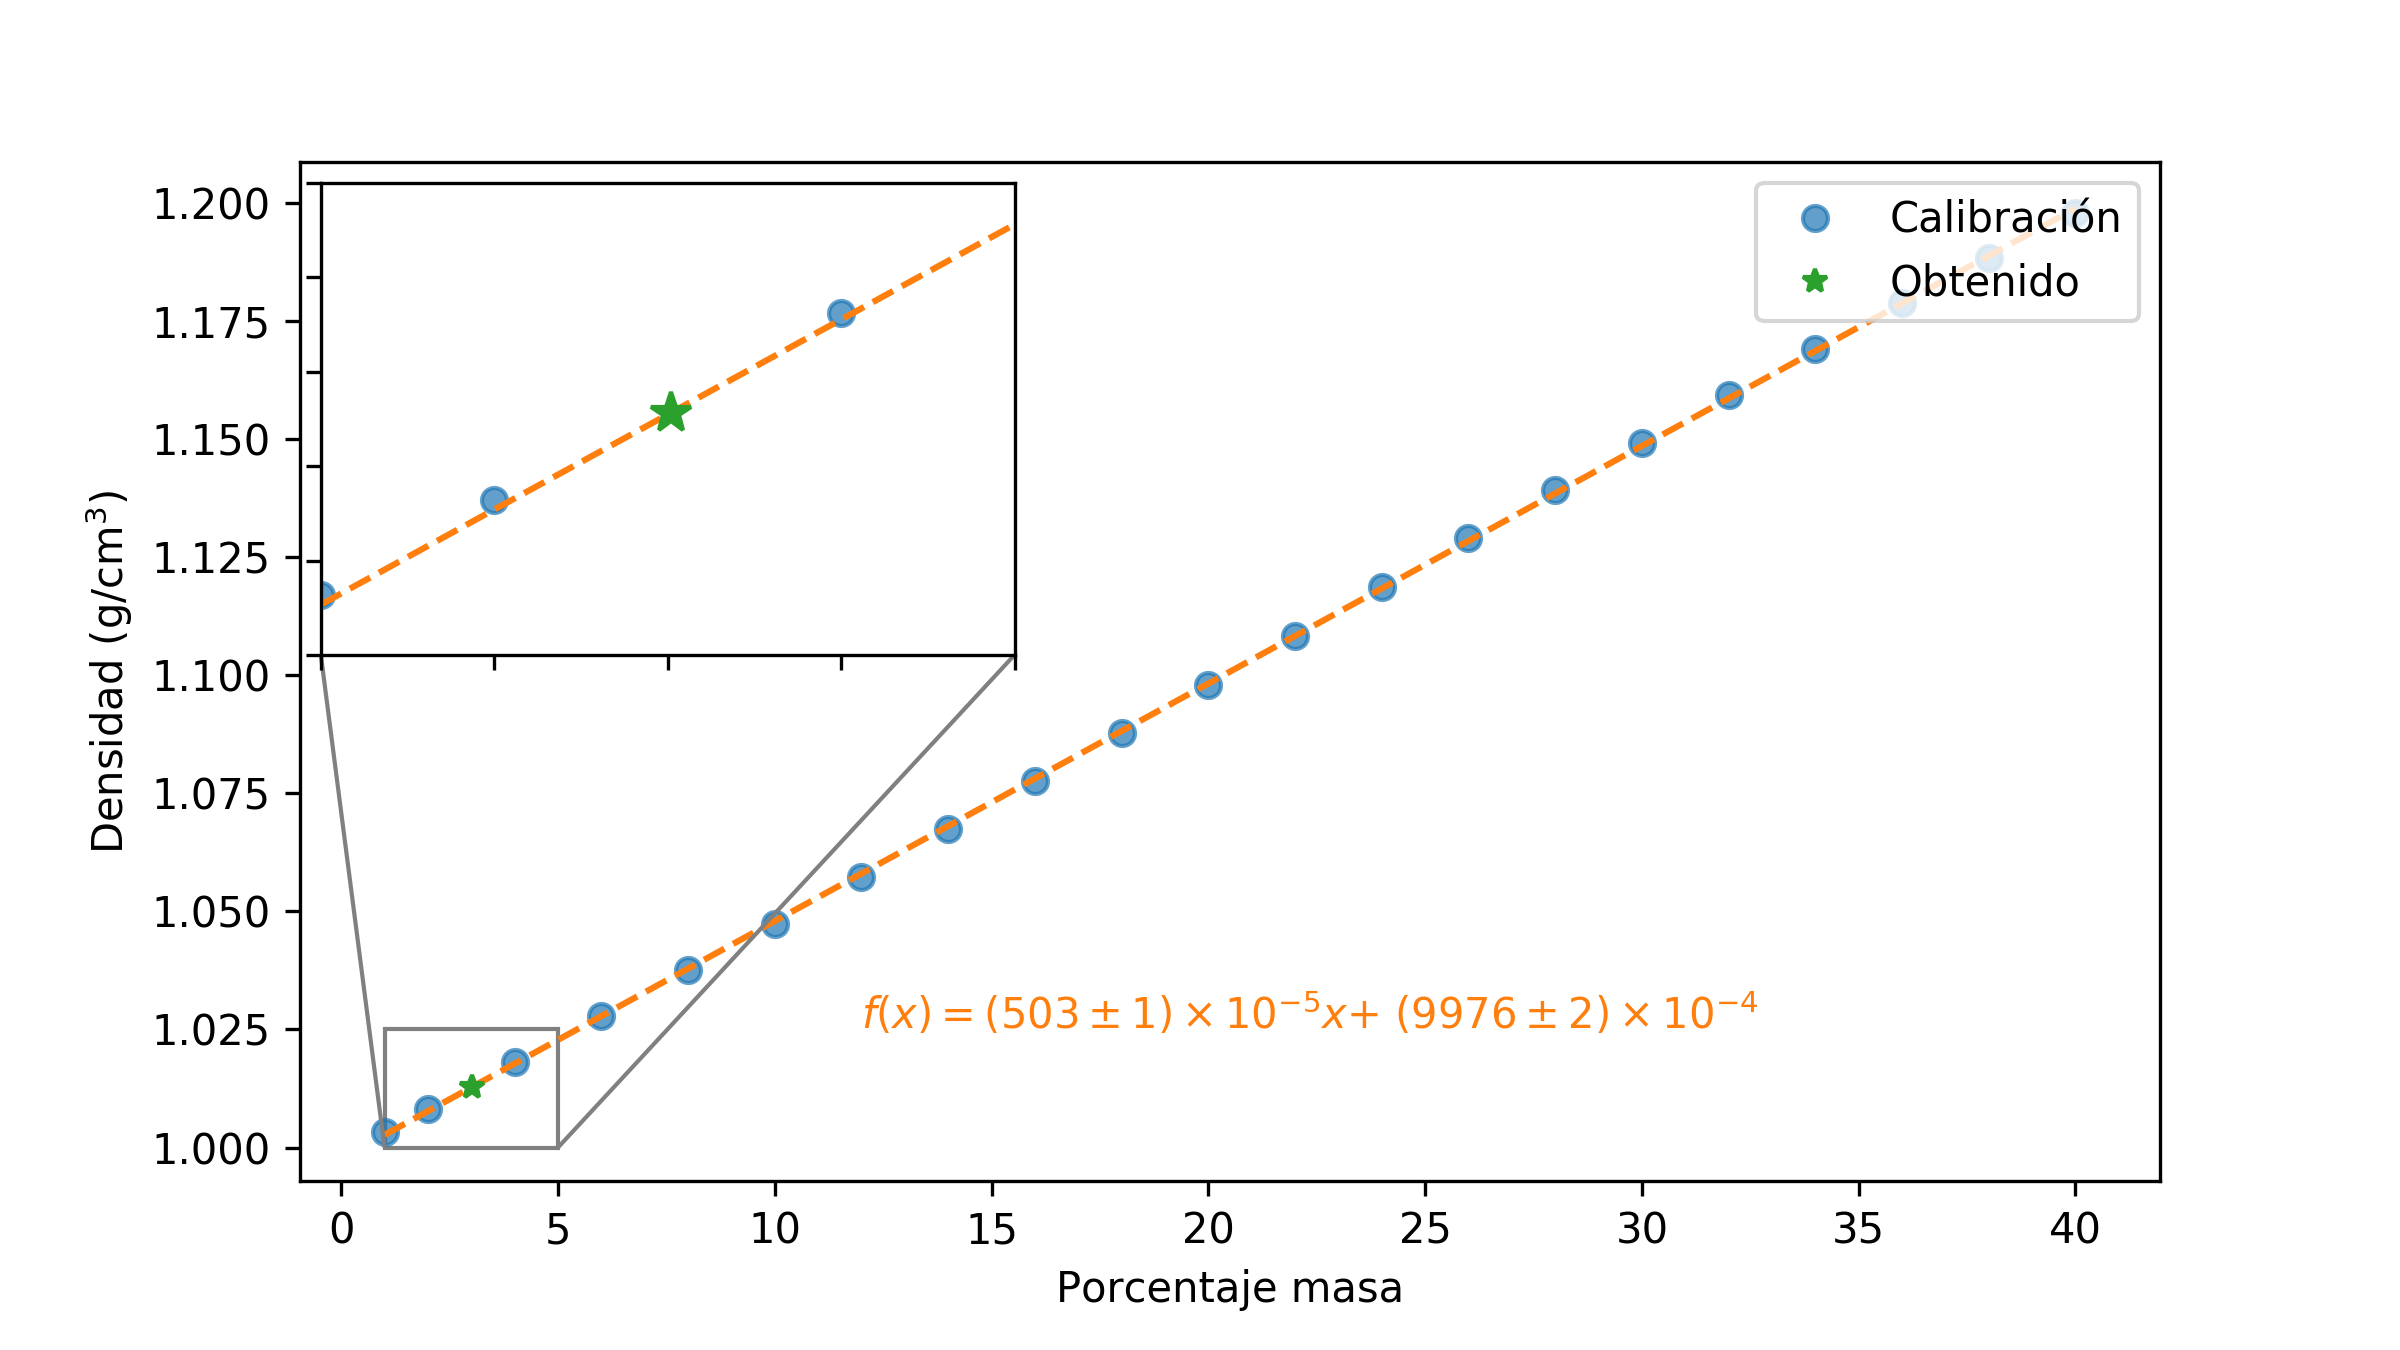
\includegraphics[width=\linewidth]{../Data/Concentration/C_HCl_initial.png}
			\caption{Determinaci\'on de la concentraci\'on de una soluci\'on de HCl usando valores de densidad reportados en la literatura \cite{perry2007perry}.}
			\label{fig: HCl_density}
		\end{figure}
		
		Para obtener la concentraci\'on $0.84 \pm 0.04$ M, se usa la siguiente ecuaci\'on, la cual relaciona la concentraci\'on en fracci\'on de masa con la molaridad $[M]$:
		\begin{equation}
			[M] = 10\dfrac{[w_t]\rho}{m_m} \qquad \text{$m_m$ la masa molecular del HCl}
		\end{equation}
		
		Se tiene entonces que la incertidumbre en la concentraci\'on estar\'a dada por:
		\begin{equation}
			\delta [M] = [M]\sqrt{\delta[w_t]^2 + \delta\rho^2} 
		\end{equation}
		
		Una al\'icuota de 0,0297 g de esta soluci\'on fue disuelta en 99,5553 g de agua, dando lugar a una soluci\'on 0,2469 mM. En la cual, la concentraci\'on final se calcula a partir de las densidades de las soluciones inicial ($\rho_s$) y final ($\rho_f$), las masas de agua ($m_\text{\ce{H2O}}$) y de soluci\'on inicial ($m_s$) usando la \autoref{eq: concentracion_f}:
		\begin{equation}\label{eq: concentracion_f}
			[M]_f = [M]_i\dfrac{V_s}{V_f} = [M_i]\dfrac{m_s/\rho_s}{(m_s + m_{\text{\ce{H2O}}})/\rho_f} =  [M]_i\left(\dfrac{m_s}{m_s + m_{\text{\ce{H2O}}}}\right)\left(\dfrac{\rho_s}{\rho_f}\right)
		\end{equation}
		
		Las densidades de las soluciones inicial y final se muestran en la \autoref{tb: concentracion_f}.
		
	\subsection{Soluci\'on de \ce{KHCO3} 0.17 mM}
	En un bal\'on aforado de 10 mL fueron adicionados 0,10143 g de \ce{KHCO3}, junto con 9,93551 g de \ce{H2O}. La densidad fue medida a 25 $^\circ$C y su valor fue 1,003662 g/cm$^3$. La concentraci\'on de esta soluci\'on se calcul\'o usando la siguiente ecuaci\'on:
	\begin{equation}
		[M] = \dfrac{n}{V} = \dfrac{m\rho}{m_m(m + m_{\ce{H2O}})}
	\end{equation}

	Obteniendo un valor de $0.10131\pm 0.00001$ M, para la cual la incertidumbre se calcula usando:
	\small
	\begin{equation}
		\delta[M] = \sqrt{\frac{m^{2}}{m_m^{2} \left(m + m_{\text{\ce{H2O}}}\right)^{2}}\delta\rho^{2} + \frac{\rho^{2} m_{\text{\ce{H2O}}}^{2}}{m_m^{2} \left(m + m_{\text{\ce{H2O}}}\right)^{4}}\delta m^{2} + \frac{\rho^{2} m^{2}}{m_m^{2} \left(m + m_{\text{\ce{H2O}}}\right)^{4}}\delta{m_{\text{\ce{H2O}}}}^{2}}
	\end{equation}
	\normalsize
	
	Posteriormente se tom\'o una al\'icuota de 0,1709 g, que fue dilu\'ida en 99,5657 g de agua. Usando la \autoref{eq: concentracion_f}, se obtiene una concentraci\'on de 0,17265 mM. El resumen de las cantidades usadas para la diluci\'on de las soluciones de \'acido y bicarbonato, as\'i como las densidades obtenidas a 20 $^\circ$C se muestran en la \autoref{tb: concentracion_f}.
	\begin{table}[h]
		\centering
		\caption{Densidades y masas medidas para preparar las soluciones con concentraciones 0,25 mM y 0,17 mM para el HCl y \ce{KHCO3} correspondientemente.}
		\small
		\begin{tabular}{c|cccccc}
			\hline
			& $\mathbf{[M]_i}$ (M) & $\mathbf{m_s}$ (g) & $\mathbf{m_{\text{H2O}}}$ (g) & $\bm{\rho_s}$ (g/cm$^3$)& $\bm{\rho_f}$ (g/cm$^3$) & $\mathbf{[M]_f}$ (mM) \\
			\hline
			\textbf{\ce{HCl}} & $0.84 \pm 0.04$ & $0.0297$ & $99.5553$ & $1.012832$ & $0.998205$ & $0.25$ \\
			\textbf{\ce{KHCO3}} & $0.10131\pm 0.00001$ & $0.1709$ & $99.5657$ & $1.003662$ & $0.998215$ & $0.17265$ \\
			\hline
		\end{tabular}
		\label{tb: concentracion_f}
	\end{table}
	
	
\subsection{Realizaci\'on del experimento}\label{sec: method}
	El m\'etodo experimental est\'a dividido en cuatro partes:
	\begin{enumerate}
		\item \textbf{Pause}: En la etapa inicial del experimento se busca medir el estado de la línea base por 120 minutos consecutivos.
		\item \textbf{Baseline}: Luego de tener datos sobre el estado sin perturbar del sistema, se realiza una calibración dinámica para obtener un ajuste fino de los parámetros de ganancia y nivel del cero de la señal. 
		\item \textbf{Pause:} En este punto se realiza una calibraci\'on est\'atica para confirmar que la calibraci\'on din\'amica fue correcta. Para esto, se aplican 300 $\mu$W sobre la celda por 30 minutos, posteriormente se retira la potencia y se esperan 50 minutos para la estabilizaci\'on de la linea base.
		\item \textbf{Main:} Una vez estabilizada la linea base, se realizan 30 inyecciones sucesivas con 10 minutos de espera entre cada inyecci\'on, la velocidad de inyecci\'on es de 50,018 $\mu/s$ y el volumen de inyecci\'on es de 51,185 $\mu$L.
	\end{enumerate}

	En la celda de medición fueron adicionados 1,6029 g de la solución de \ce{KHCO3} 0,17265 mM, y la jeringa fue cargada con 2,0 mL de la soluci\'on de HCl 0,2469 mM, ambas soluciones fueron desgasificadas por 15 minutos a 44 \grad{} en un sonicador, adem\'as, la temperatura del ba\~no t\'ermico se mantuvo en $25.05 \pm 0.06$ $^\circ$C a lo largo del experimento.
	
\subsection{Resultados}
	Considerando un proceso a presi\'on constante, se tiene una expresi\'on que relaciona la potencia con la entalp\'ia por inyecci\'on, donde el signo negativo en la \autoref{eq: heat} viene de la polarizaci\'on del equipo, lecturas de potencia positivas corresponden con reacciones exot\'ermicas:
	\begin{equation}\label{eq: heat}
		\int\limits_t^{t + \Delta t_\text{iny}} Pdt = Q_\text{iny} = -\Delta H_\text{iny}
	\end{equation}
	
	Sin embargo
	
	\begin{figure}[h]
		\centering
		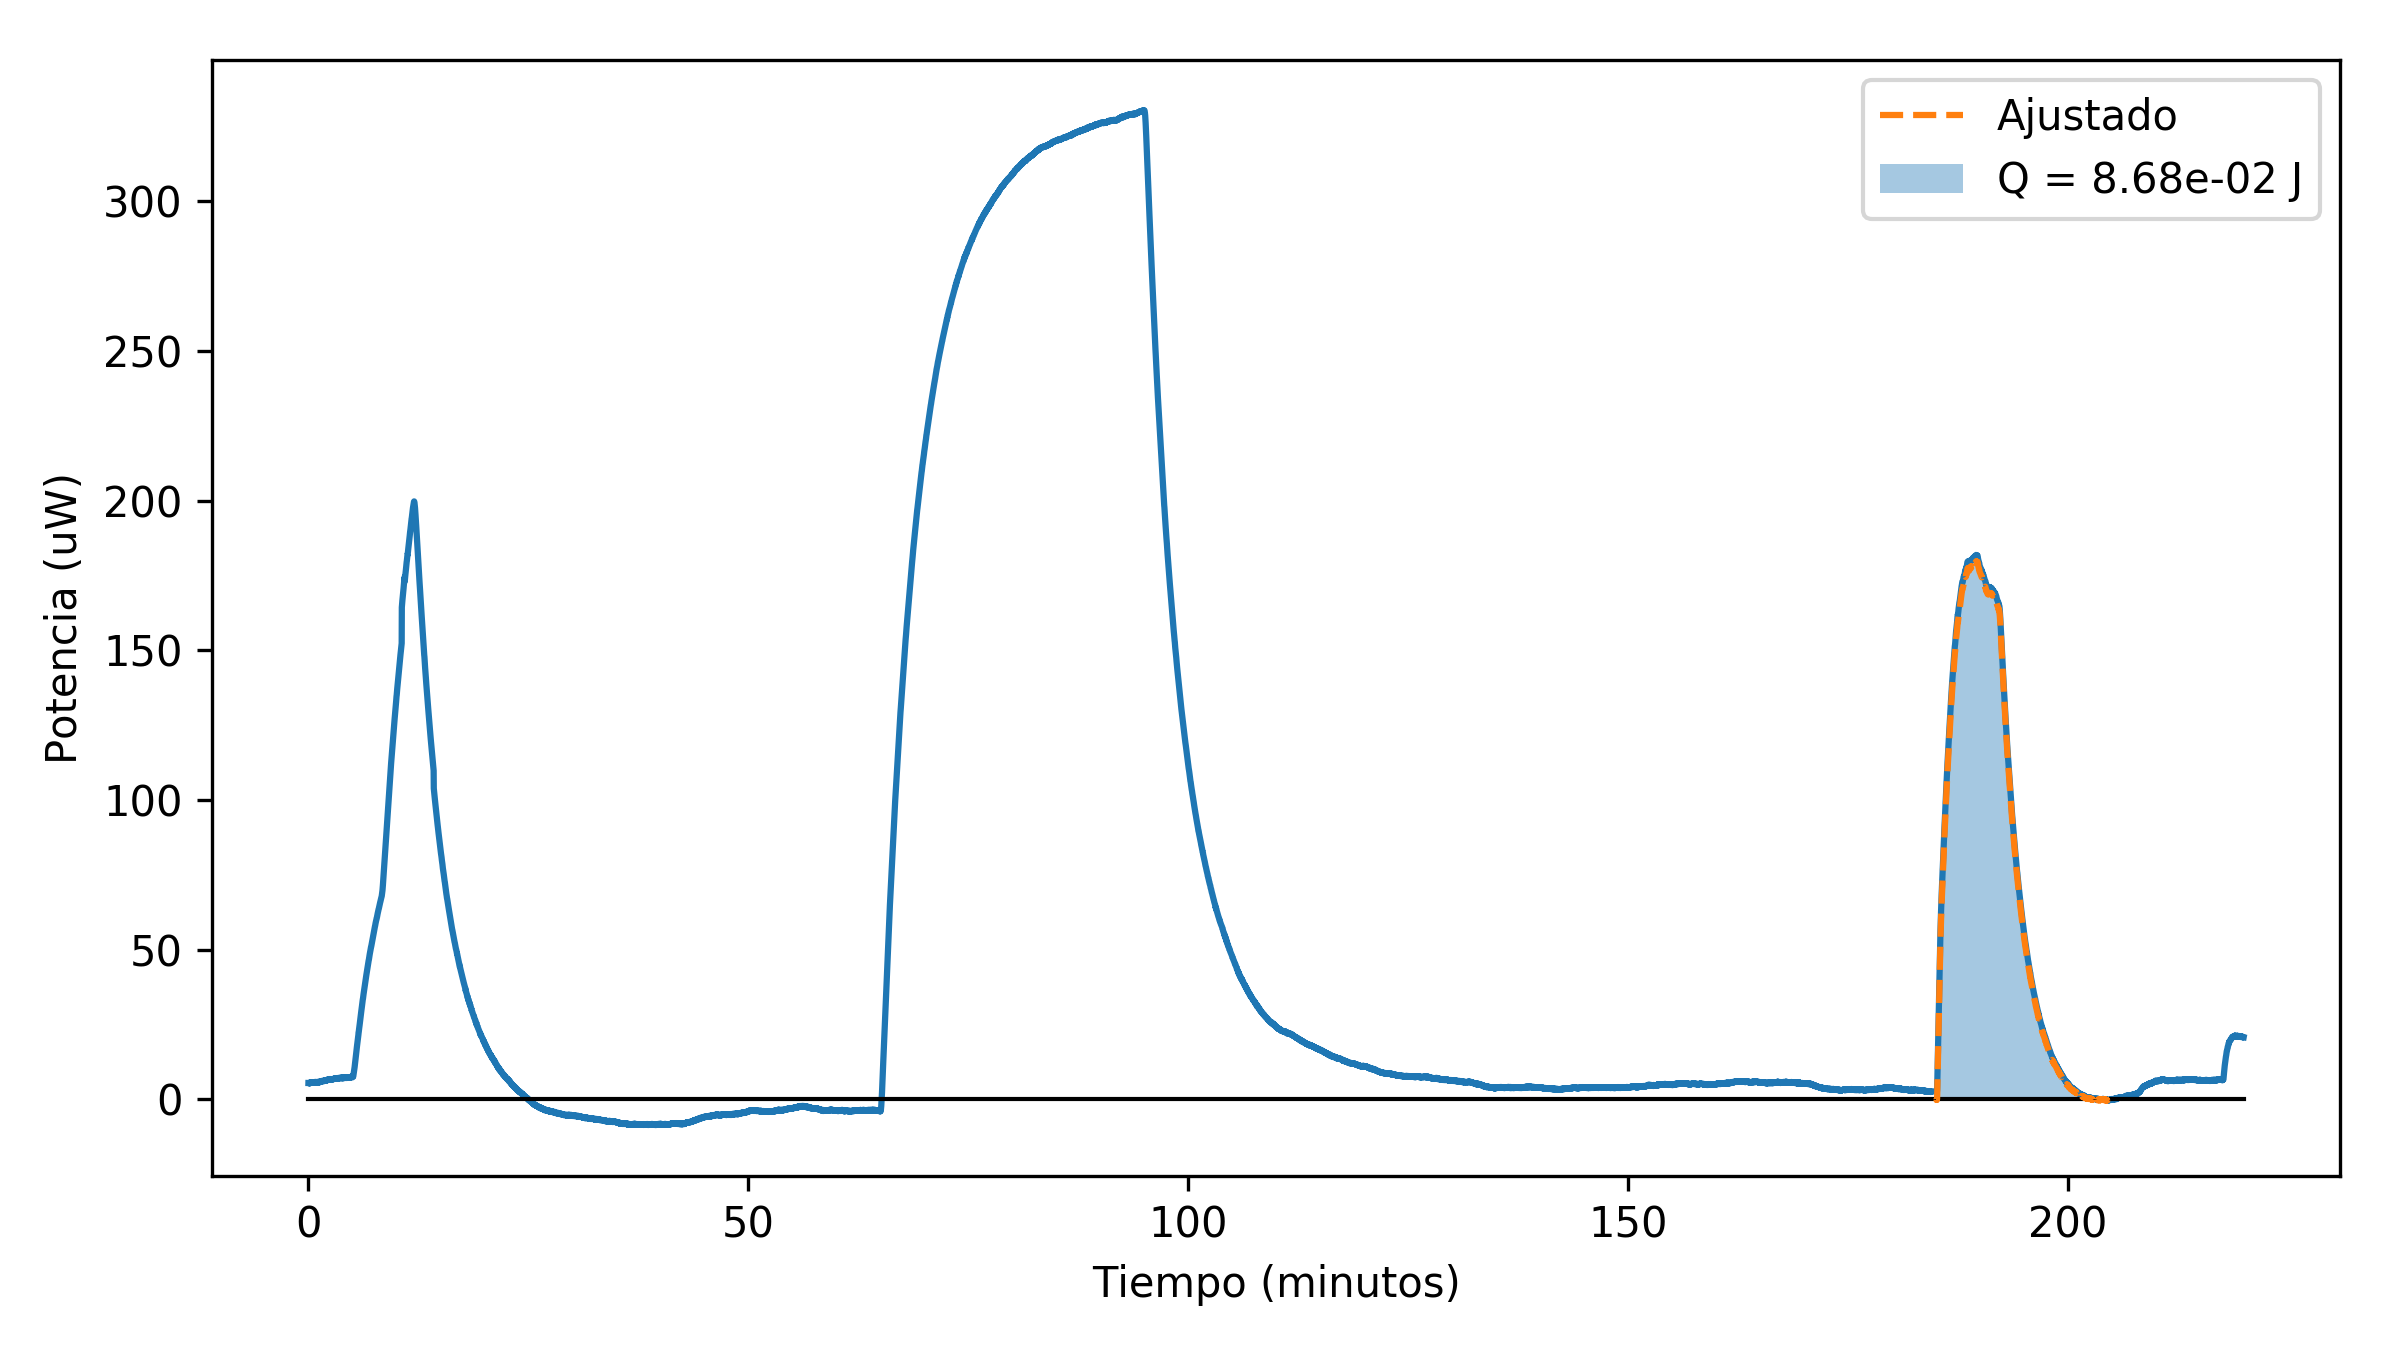
\includegraphics[width=\linewidth]{../Data/ChemicalCalibrations/HCl}
		\caption{Las se\~nales entre 0 y 100 minutos, corresponden con una calibraci\'on din\'amica y est\'atica. Posteriormente, las 2 inyecciones.}
		\label{fig: HClResults}
	\end{figure}

	Dado que el calor\'imetro registra valores de potencia y esta corresponde con energ\'ia por unidad de tiempo, es necesario integrar en el tiempo la se\~nal obtenida para cada inyecci\'on, de esta manera se determina el calor generado por cada una de estas. Adem\'as, de la primera ley de la termodin\'amica se tiene que $U = Q - \int pdV$ y $H\equiv U+pV$, la entalp\'ia est\'a dada por:
	\begin{equation}
		\Delta H = Q + V\Delta p
	\end{equation}
	
	
	
	Para obtener la entalp\'ia de la reacci\'on se grafican las entalp\'ias de inyecci\'on en funci\'on de la raz\'on molar, y se toma la diferencia entre la as\'intota inicial y final, cuyo valor corresponde con la entalp\'ia total de la reacci\'on \cite{nanoitc}. Posteriormente, para determinar la entalp\'ia molar se divide el resultado anterior por el n\'umero de moles de titulante usado. Por otro lado se tiene que en el punto de equivalencia la pendiente corresponde con la constante de afinidad, para la cual se cumple la siguiente relaci\'on \cite{matsuyama2017isothermal, velazquez2006isothermal, nanoitc}: 
	\begin{equation}\label{eq: gibbs}
		\Delta G = -RT\ln K_a
	\end{equation}
	
	Donde $K_a$ se denomina la constante de afinidad y se obtiene del equilibrio de la reacci\'on:
	\begin{equation}
		\ce{KHCO3(ac) + HCl(ac) <=>[K_a] H2O(l) + KCl(ac) + CO2(g)}
	\end{equation}
	
	Usando la \autoref{eq: gibbs} se obtiene el cambio en energ\'ia libre de Gibbs, lo cual a su vez permite determinar la entrop\'ia, pues de la definici\'on de esta junto con la primera ley de la termodin\'amica se obtiene:
	\begin{equation}
		G \equiv H - TS = (U + pV) - TS
	\end{equation}
	\begin{equation}
		\begin{matrix}
			dG & = & dU + pdV + VdP - SdT -TdS \\
			& = & dQ - pdV + pdV + VdP -SdT -TdS \\
			& = & (dQ + VdP) - SdT - TdS \\
			& = & dH - SdT - TdS
		\end{matrix}
	\end{equation}
	
	Lo cual para condiciones isot\'ermicas y cambios grandes ($d \rightarrow \Delta$) se reduce a: $\Delta G = \Delta H - T\Delta S$, de donde se obtiene:
	\begin{equation}
		\Delta S = \dfrac{\Delta H - \Delta G}{T}
	\end{equation}
	
	Para poder calcular las cantidades mencionadas anteriormente, es necesario obtener la potencia de cada inyecci\'on, sin embargo, como se observa en la \autoref{fig: HClResults}, existe una segunda inyecci\'on (10 minutos despu\'es que la otra) que registra una gran potencia, posterior a esta se desequilibra el calor\'imetro.

	La energ\'ia medida en las inyecciones se calcula con la \autoref{eq: heat}. Entre $t = 127$ min, hasta $t + \Delta T=141$ min, como se muestra en color nar\'anja en la \autoref{fig: HClResults}, dando lugar a un valor de 45,88 mJ. Considerando ahora que se agregaron 102,37 $\mu$L (2 inyecciones) de una soluci\'on 0,2469 mM de HCl, fueron adicionados 25,28 nmoles de HCl, por lo cual se tiene que $Q = \Delta H = -1815$ kJ/mol, valor que es muy superior al esperado de $-9.0 \pm 0.9$ kJ/mol \cite{nanoitc}. Adem\'as, dicho resultado no explica la desestabilizaci\'on posterior del calor\'imetro, as\'i como la no observaci\'on de m\'as inyecciones. Por lo cual se procedi\'o a probar el sistema la disoluci\'on de propanol en agua.
	
 
% !TeX spellcheck = es_ES
% Chapter 1

%\chapter{Chapter Title Here} % Main chapter title
%
%\label{Chapter1} % For referencing the chapter elsewhere, use \ref{Chapter1} 

%----------------------------------------------------------------------------------------

% Define some commands to keep the formatting separated from the content 
%\newcommand{\keyword}[1]{\textit{#1}}
%\newcommand{\tabhead}[1]{\textbf{#1}}
%\newcommand{\code}[1]{\texttt{#1}}
%\newcommand{\file}[1]{\texttt{\bfseries#1}}
%\newcommand{\option}[1]{\texttt{\itshape#1}}

%----------------------------------------------------------------------------------------

\chapter{Conclusiones}


		

%----------------------------------------------------------------------------------------
%	THESIS CONTENT - APPENDICES
%----------------------------------------------------------------------------------------

% Include the appendices of the thesis as separate files from the Appendices folder
% Uncomment the lines as you write the Appendices

%\include{Appendices/AppendixA}
%\include{Appendices/AppendixB}
%\include{Appendices/AppendixC}

%----------------------------------------------------------------------------------------
%	BIBLIOGRAPHY
%----------------------------------------------------------------------------------------

\printbibliography[heading=bibintoc, title={Referencias}]

\appendix % Cue to tell LaTeX that the following "chapters" are Appendices
% !TeX spellcheck = es_ANY
% Chapter 1

%\chapter{Chapter Title Here} % Main chapter title
%
%\label{Chapter1} % For referencing the chapter elsewhere, use \ref{Chapter1} 

%----------------------------------------------------------------------------------------

% Define some commands to keep the formatting separated from the content 
%\newcommand{\keyword}[1]{\textit{#1}}
%\newcommand{\tabhead}[1]{\textbf{#1}}
%\newcommand{\code}[1]{\texttt{#1}}
%\newcommand{\file}[1]{\texttt{\bfseries#1}}
%\newcommand{\option}[1]{\texttt{\itshape#1}}

%----------------------------------------------------------------------------------------

\chapter{Anexos}
	\section{Firmware microcontrolador}
		\lstinputlisting[language = C]{../MeasuringTools/micro/main.c}
	
	\section{Software de Temperatura}
		\subsection{Comunicaciones}
			\lstinputlisting{../MeasuringTools/TemperatureSoft/com.py}
			
		\subsection{Interfaz gr\'afica}
			\lstinputlisting{../MeasuringTools/TemperatureSoft/gui.py}

%----------------------------------------------------------------------------------------

\end{document}  
